\section{Fit results}
\label{ref:fit:results}

The fitted yields are grouped as follows:
\Dz\muon, \Dstarp\muon, \Dstarz\muon,
signal,
four $1P$ $D^{**}$,
heavy $D^{**}$,
$DD$,
$D_s$,
combinatorial backgrounds,
and \muon misID.
The combined yields of the groups of the signal fit are reported in
\cref{tab:fit-yields} for both fit channels,
with the signal yields blinded (replaced with a random number).

\begin{table}[!ht]
    \centering
    \caption{Fitted yields of the signal fit.}
    \label{tab:fit-yields}

\begin{subtable}[b]{0.5\textwidth}
    \centering

\begin{tabular}[b]{lr}
\hline
 \bfseries Group               &    \bfseries Yields \\
\hline
 norm. ($D^0\mu$)    &   445,095 \\
 norm. ($D^{*+}\mu$) &   115,124 \\
 norm. ($D^{*0}\mu$) & 1,176,363 \\
 sig. (random)       &        14 \\
 $D^{**}$            &   167,968 \\
 $D^{**}$ heavy      &    38,147 \\
 $D_s$               &     5,285 \\
 $DD$                &    96,236 \\
 comb. bkg.          &    20,596 \\
 misID               &    56,596 \\
\hline
\end{tabular}

    \caption{\Dz channel}
\end{subtable}%
%%%%
\begin{subtable}[b]{0.5\textwidth}
    \centering

\begin{tabular}[b]{lr}
\hline
 \bfseries Group               &   \bfseries Yields \\
\hline
 norm. ($D^{*+}\mu$) &  427,783 \\
 sig. (random)       &        5 \\
 $D^{**}$            &   37,181 \\
 $D^{**}$ heavy      &   12,804 \\
 $D_s$               &    3,730 \\
 $DD$                &   33,588 \\
 comb. bkg.          &   16,906 \\
 misID               &    8,175 \\
\hline
\end{tabular}

    \caption{\Dstar channel}
\end{subtable}

\end{table}


The pre-control fit results are plotted in \cref{appx:suppl:fit-pre-ctrl};
the control fit results are displayed in
\cref{fig:ctrl-1os-d0,fig:ctrl-2os-d0,fig:ctrl-dd-d0} for \Dz channel;
\cref{fig:ctrl-1os-dst,fig:ctrl-2os-dst,fig:ctrl-dd-dst} for \Dstar channel;
the signal fit results in \cref{fig:sig-d0,fig:sig-dst}
for the \Dz and \Dstar channel, accordingly.


% ctrl
\begin{figure}[!htb]
    \centering
    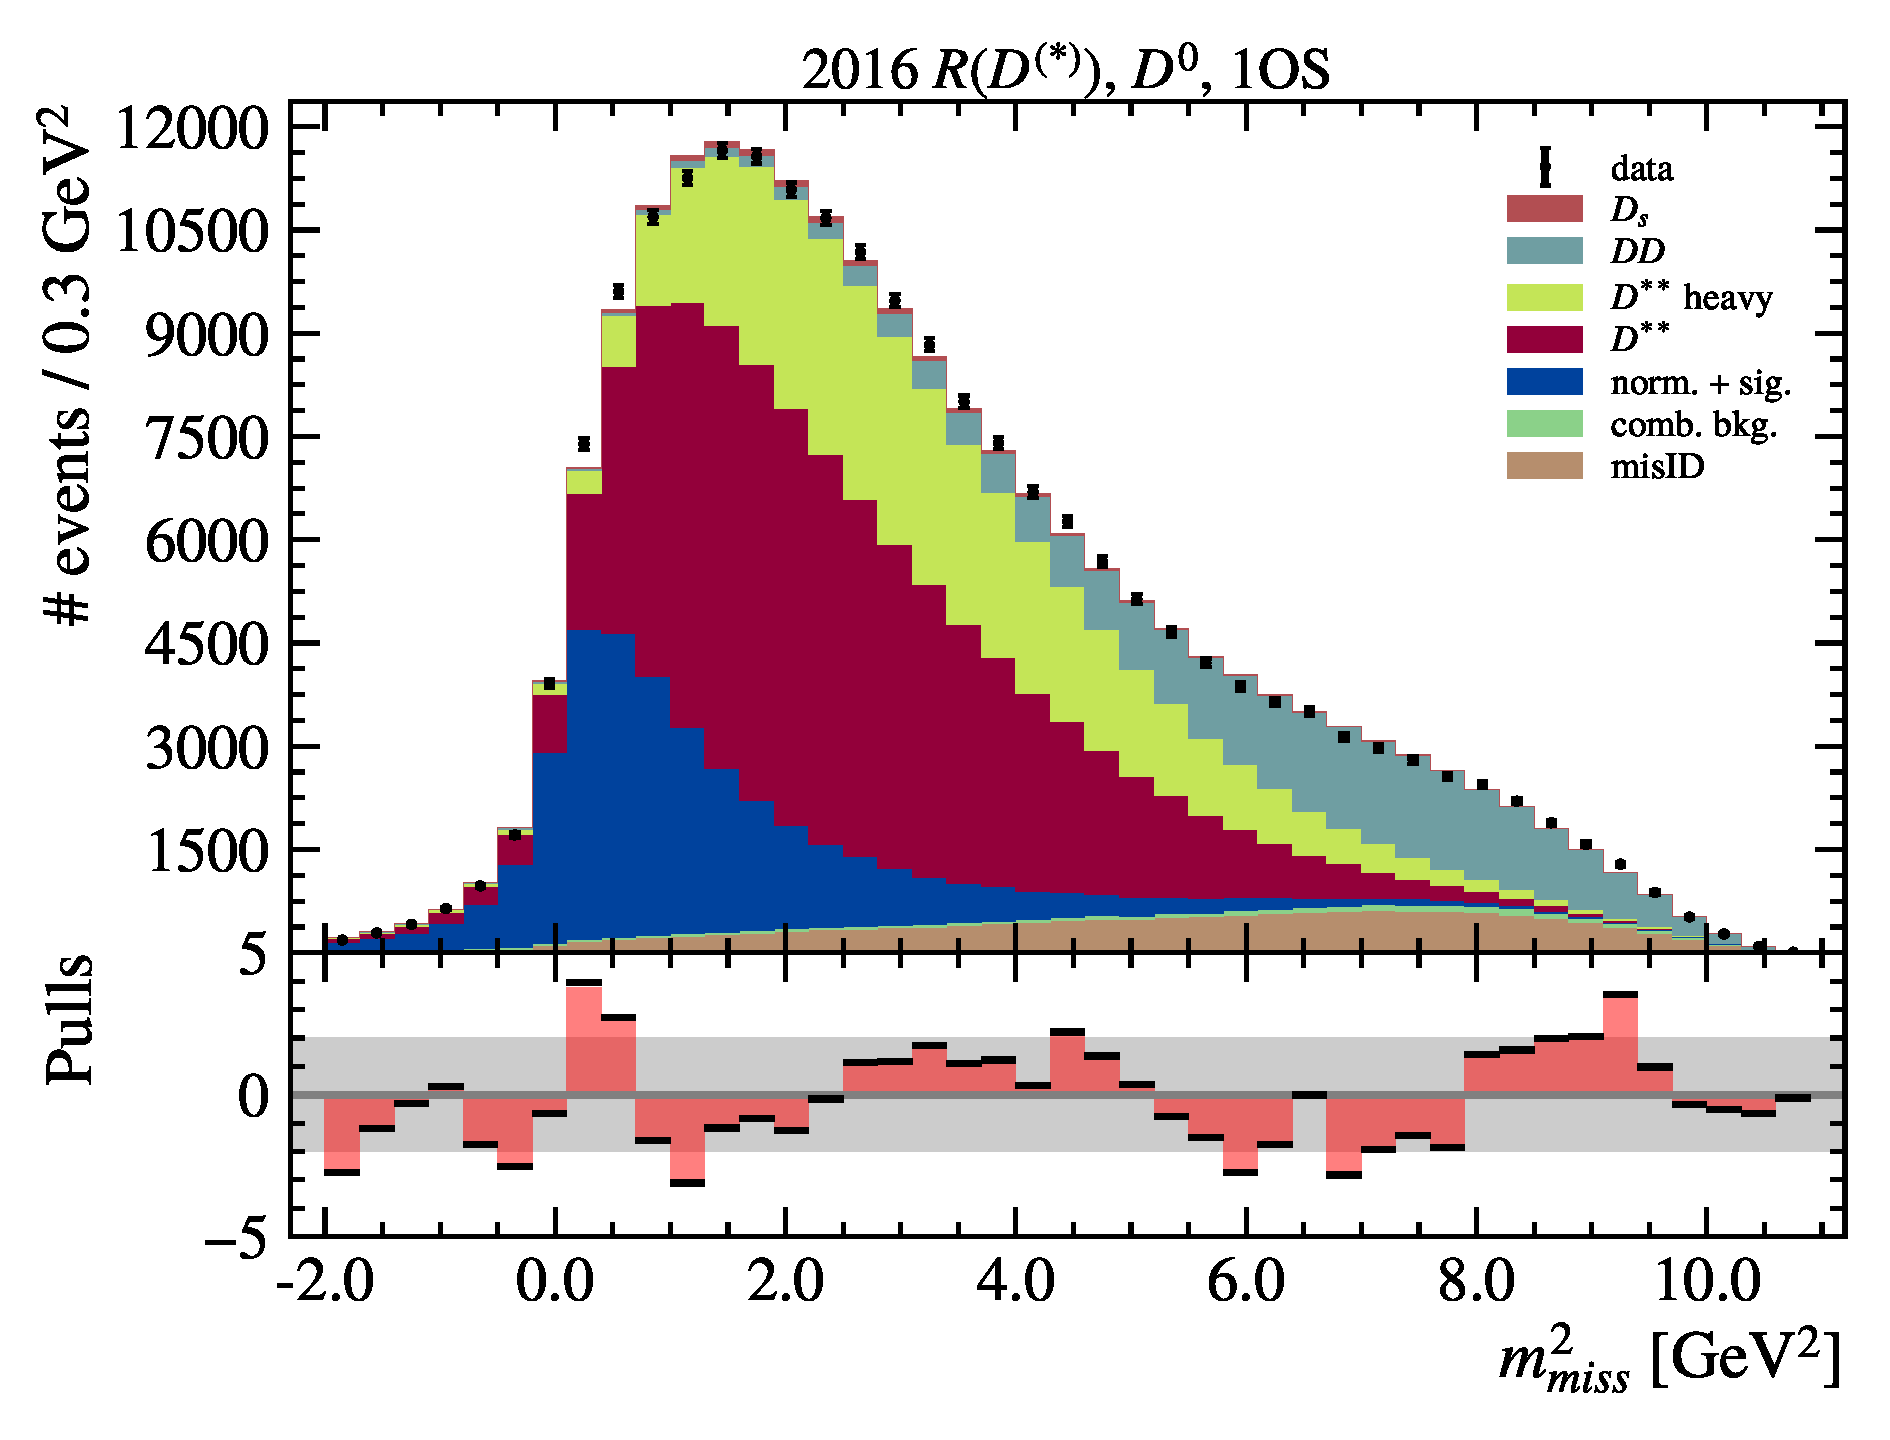
\includegraphics[width=0.32\textwidth]{./figs-fit-fit-results/ctrl-fit/stacked/fit_result-stacked-D0-1os-mmiss2.pdf}
    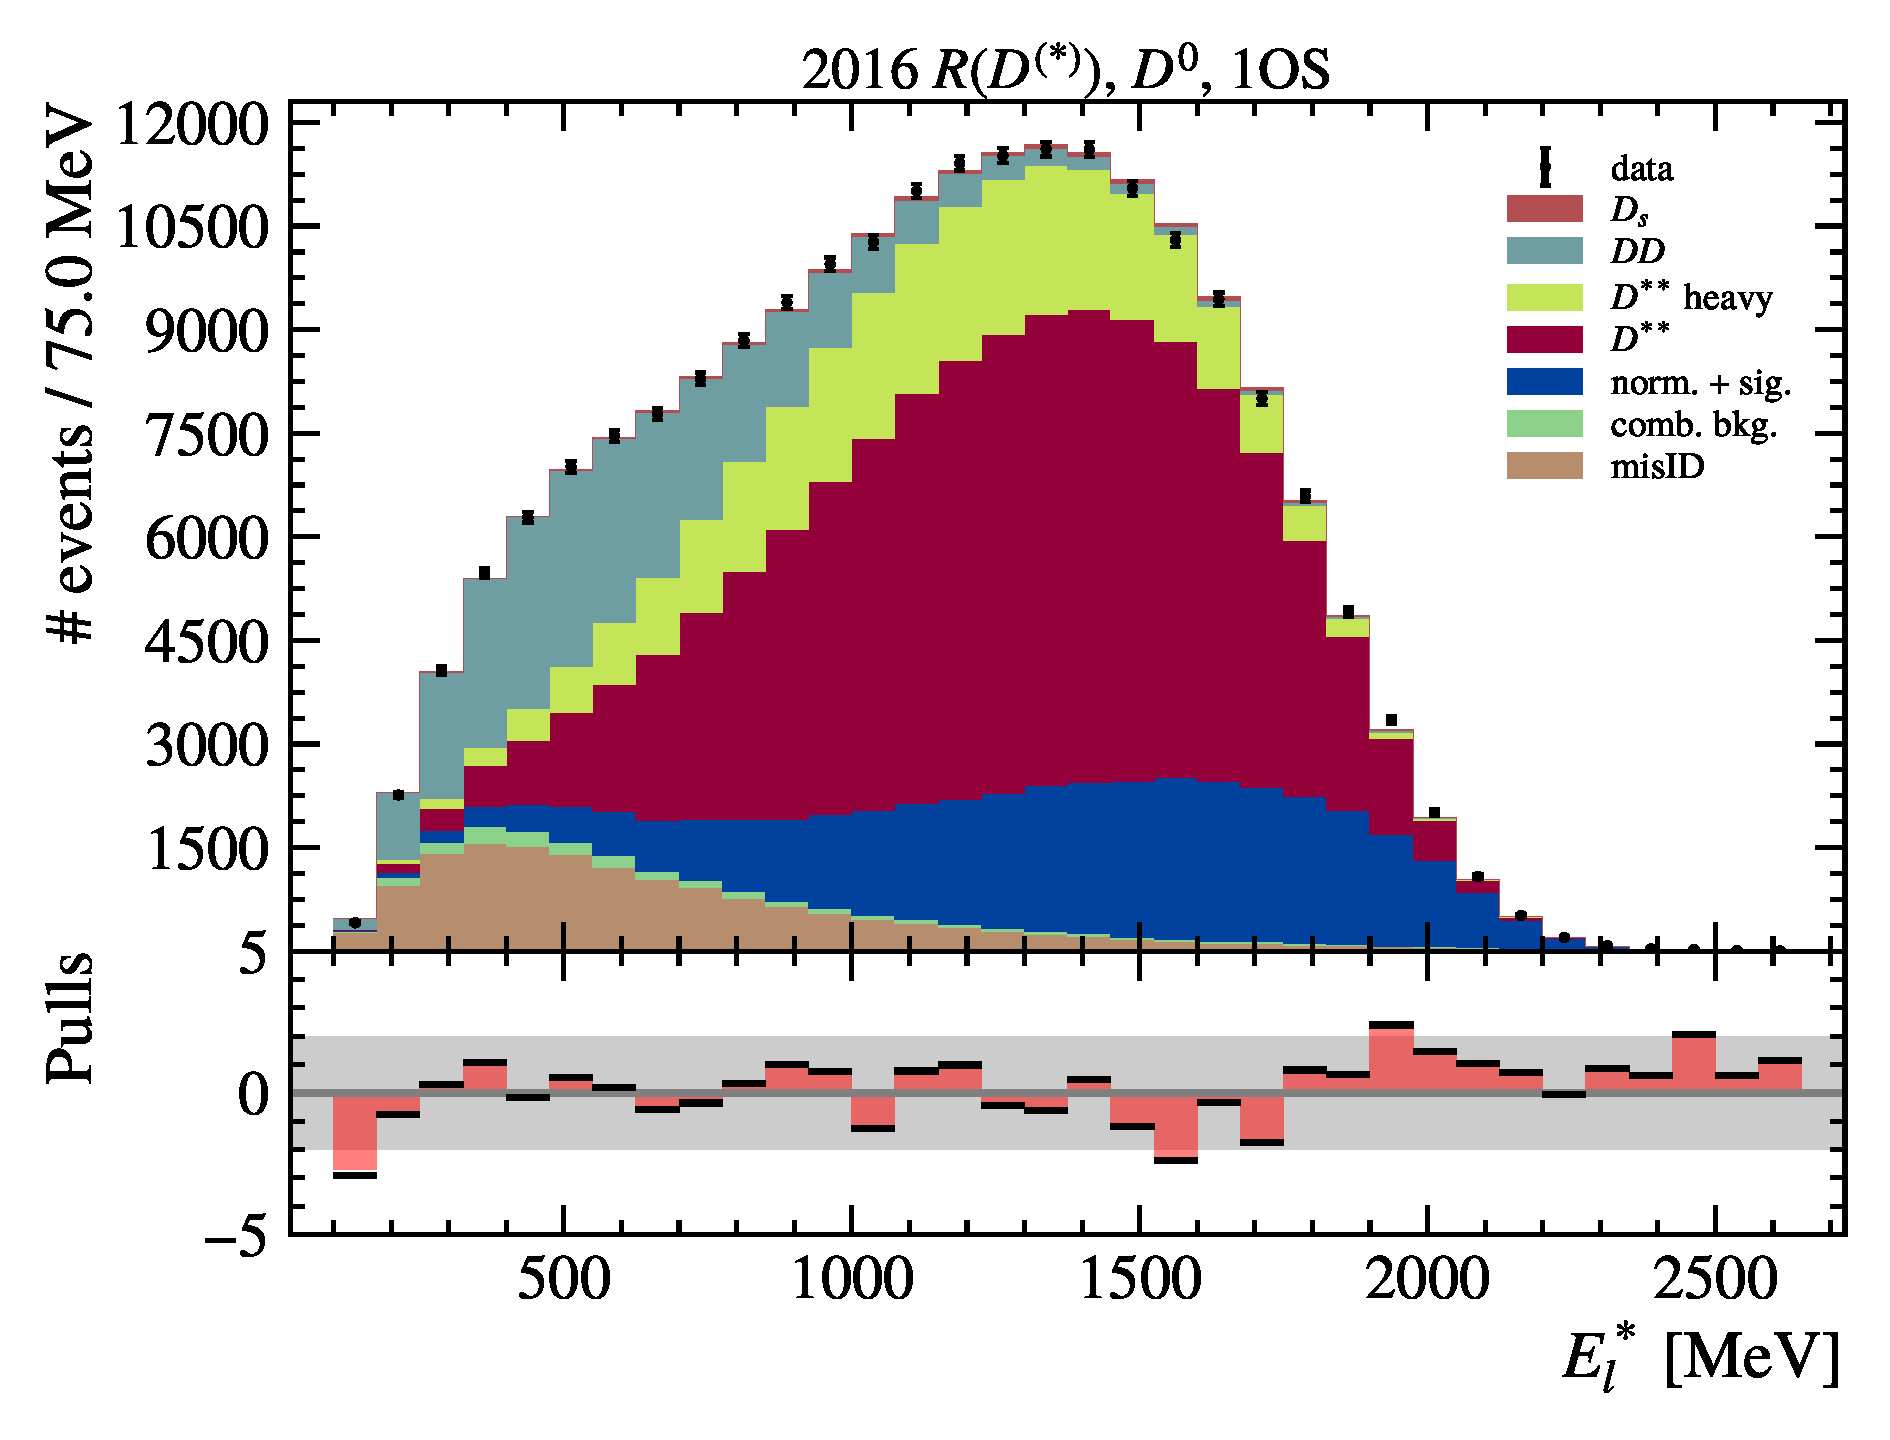
\includegraphics[width=0.32\textwidth]{./figs-fit-fit-results/ctrl-fit/stacked/fit_result-stacked-D0-1os-el.pdf}
    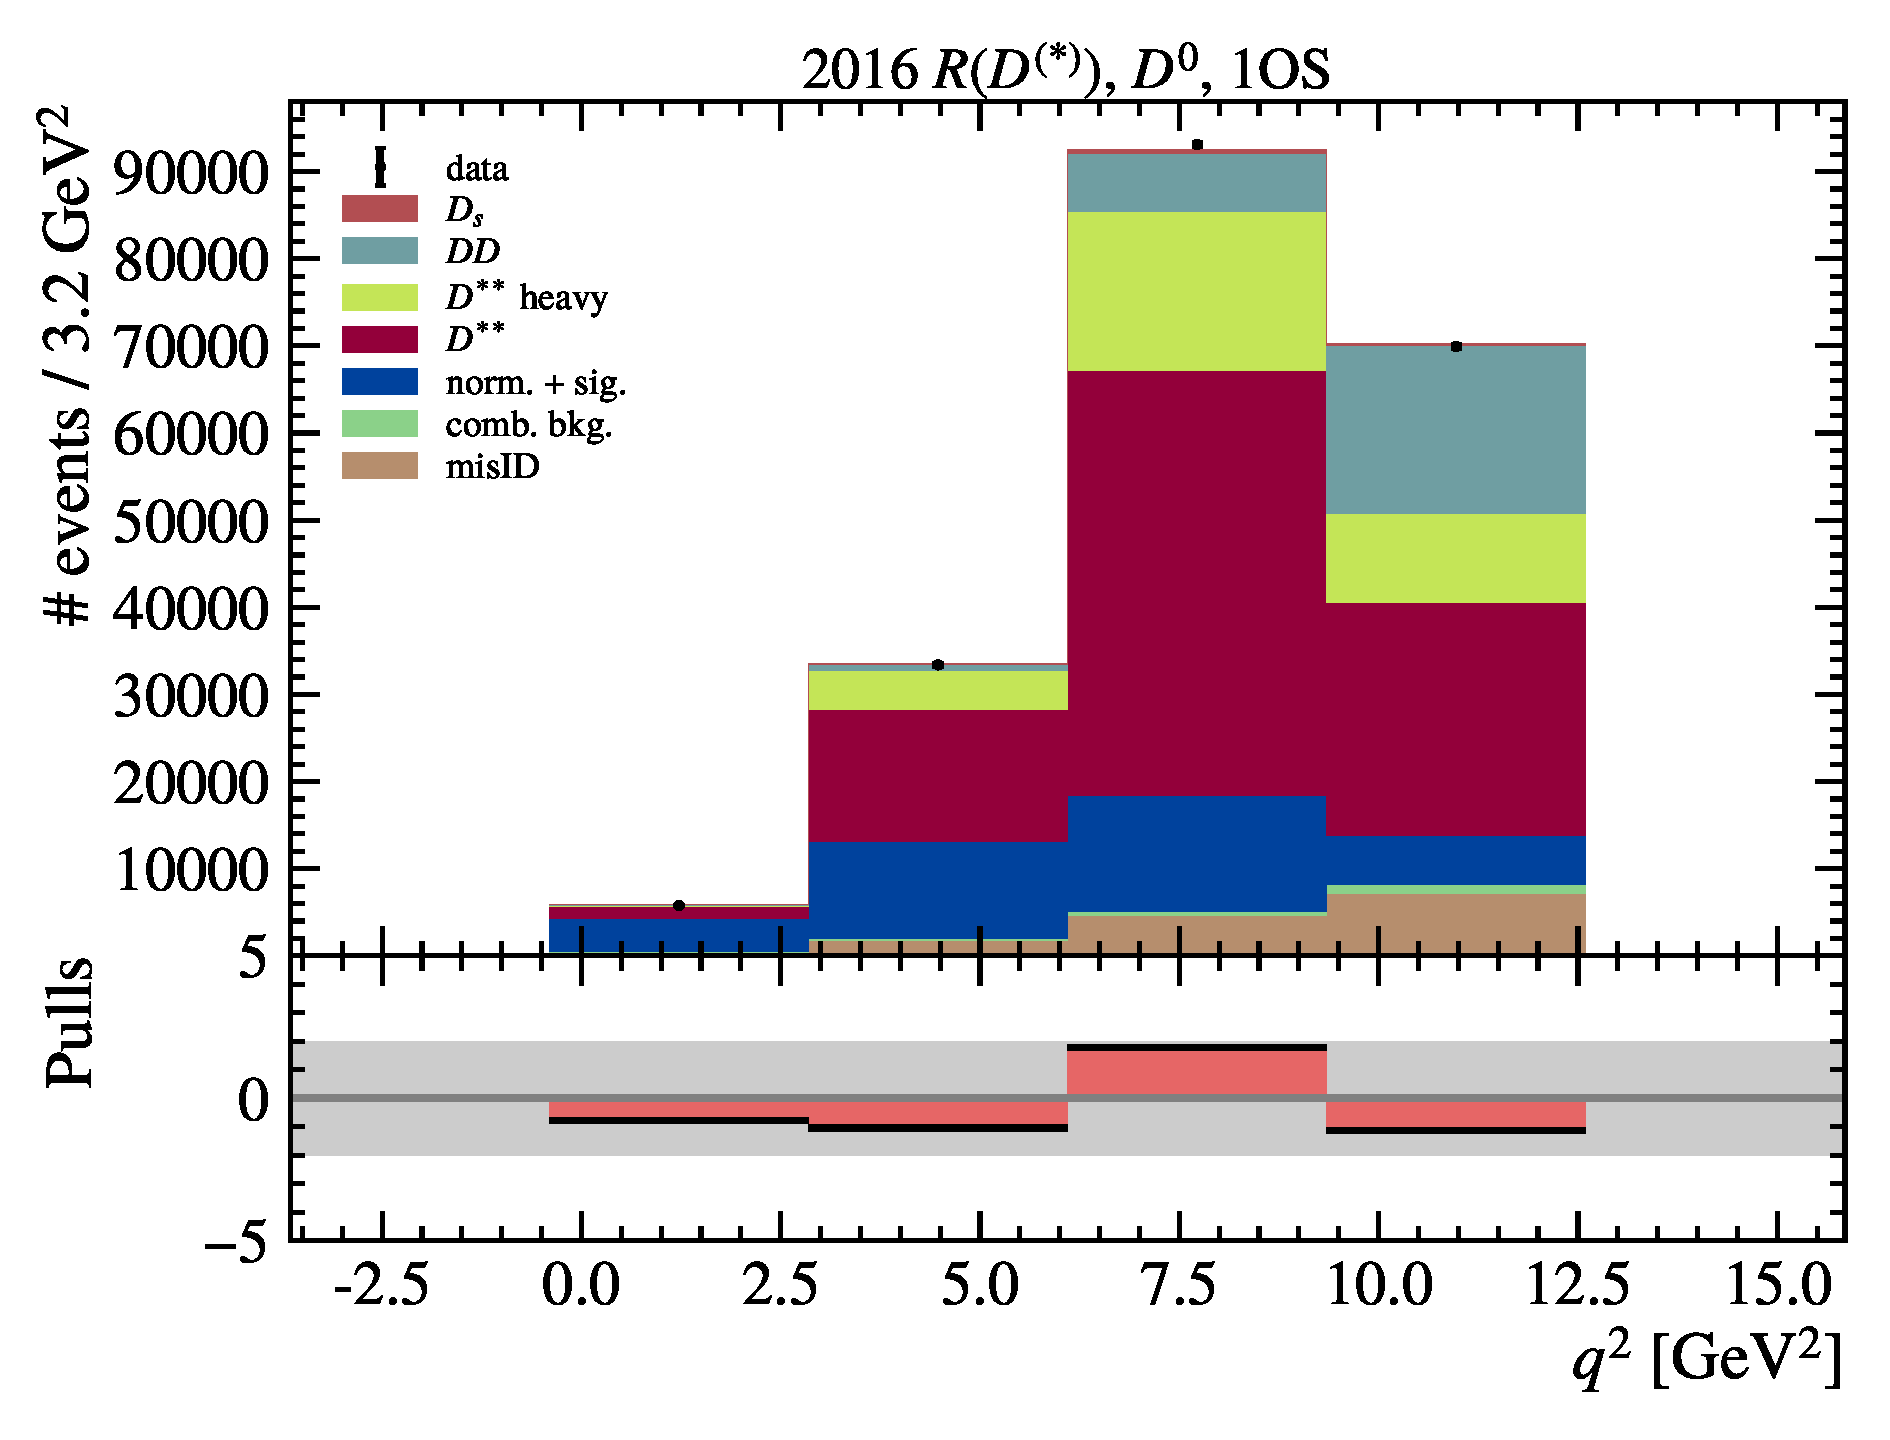
\includegraphics[width=0.32\textwidth]{./figs-fit-fit-results/ctrl-fit/stacked/fit_result-stacked-D0-1os-q2.pdf}

    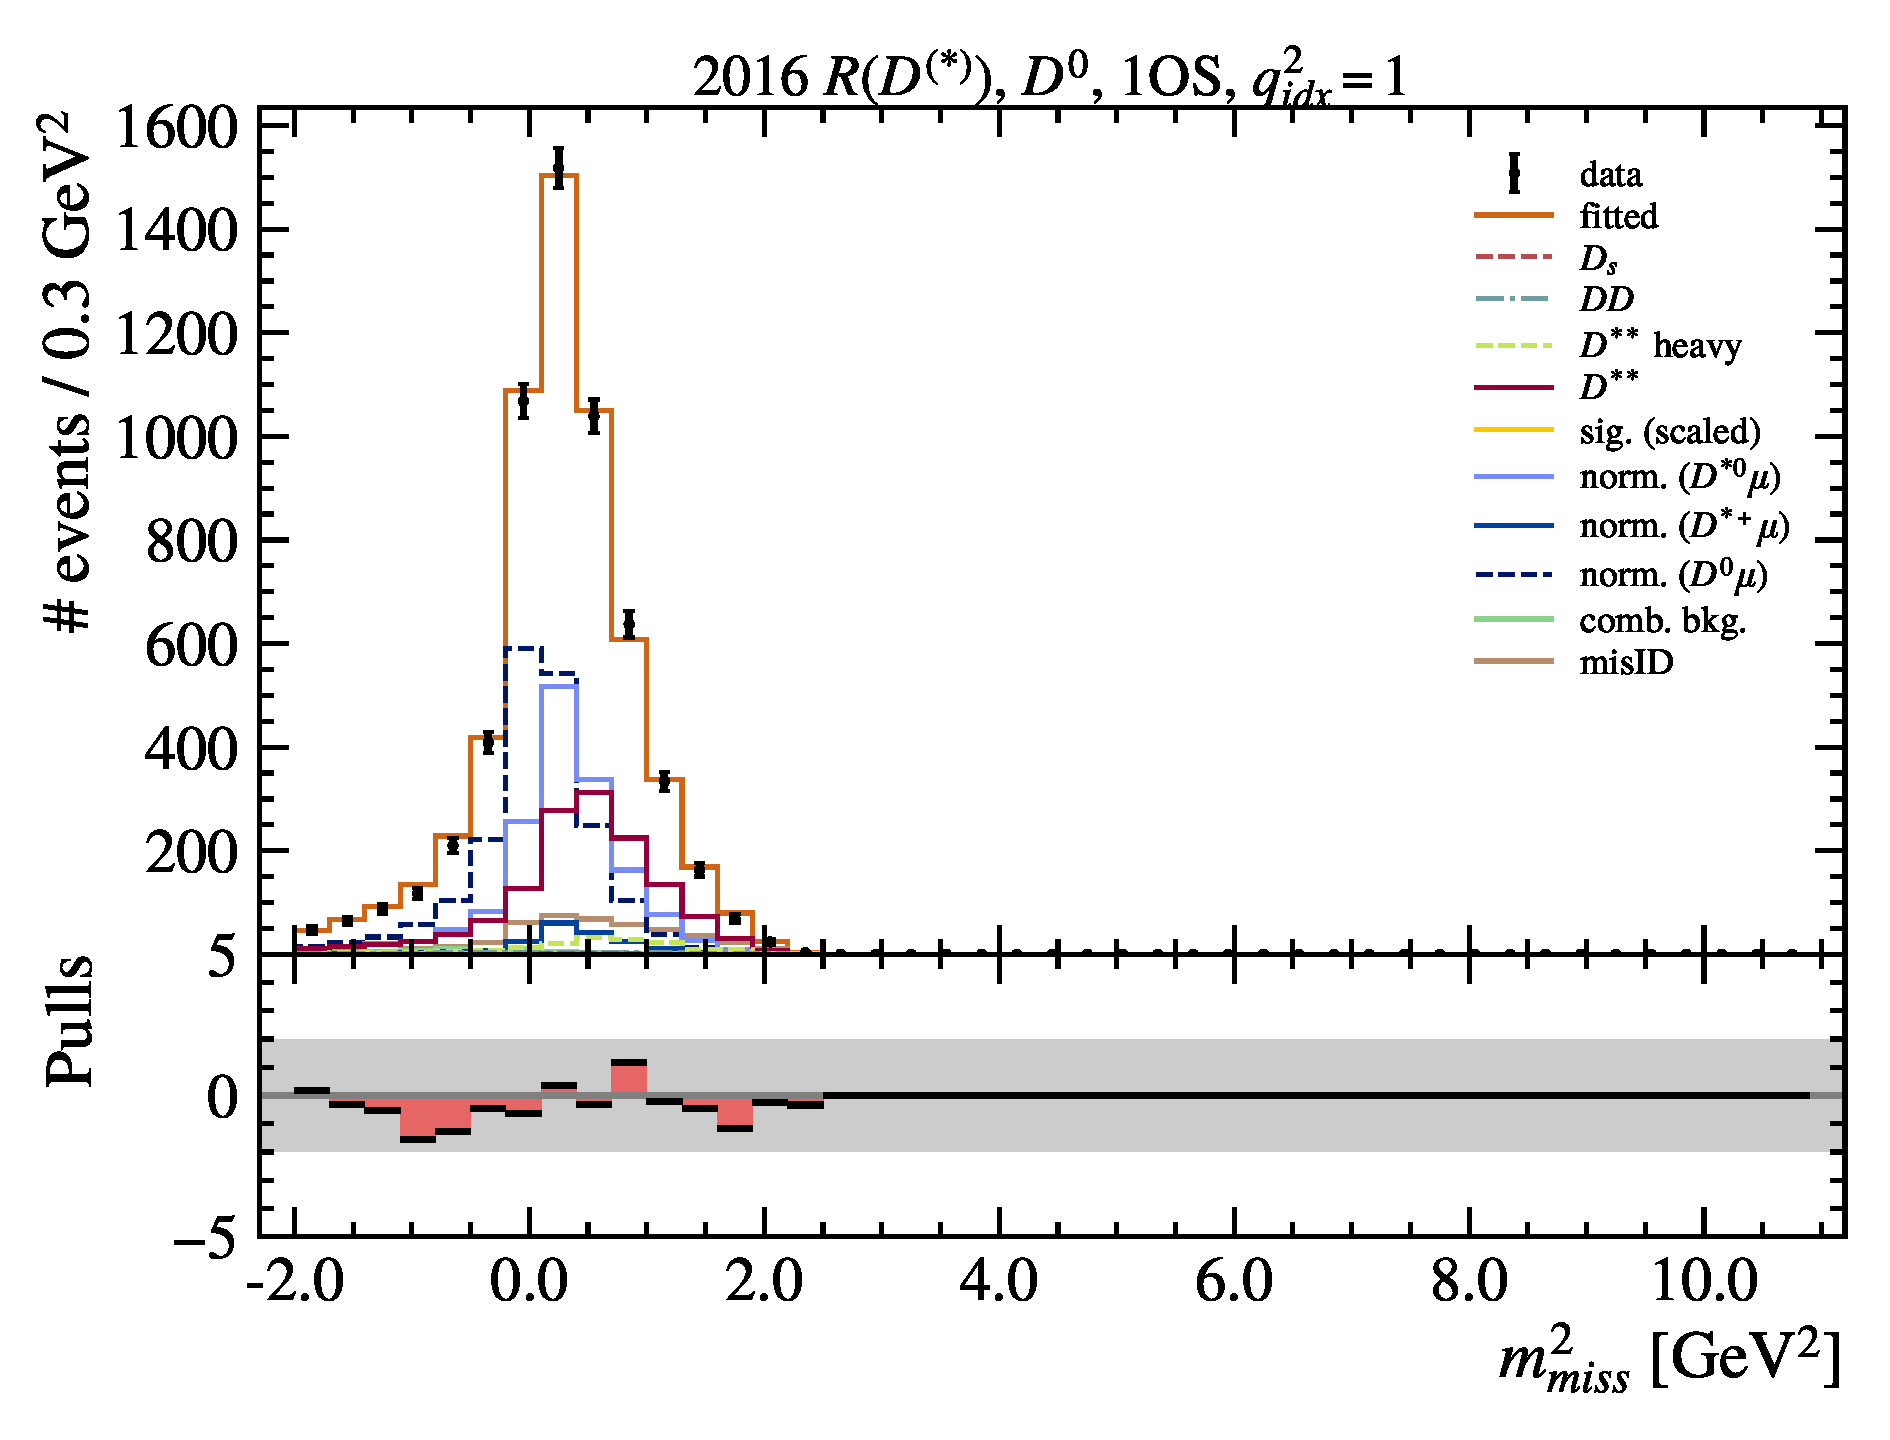
\includegraphics[width=0.24\textwidth]{./figs-fit-fit-results/ctrl-fit/lines_q2_slices/fit_result-lines_q2_idx1-D0-1os-mmiss2.pdf}
    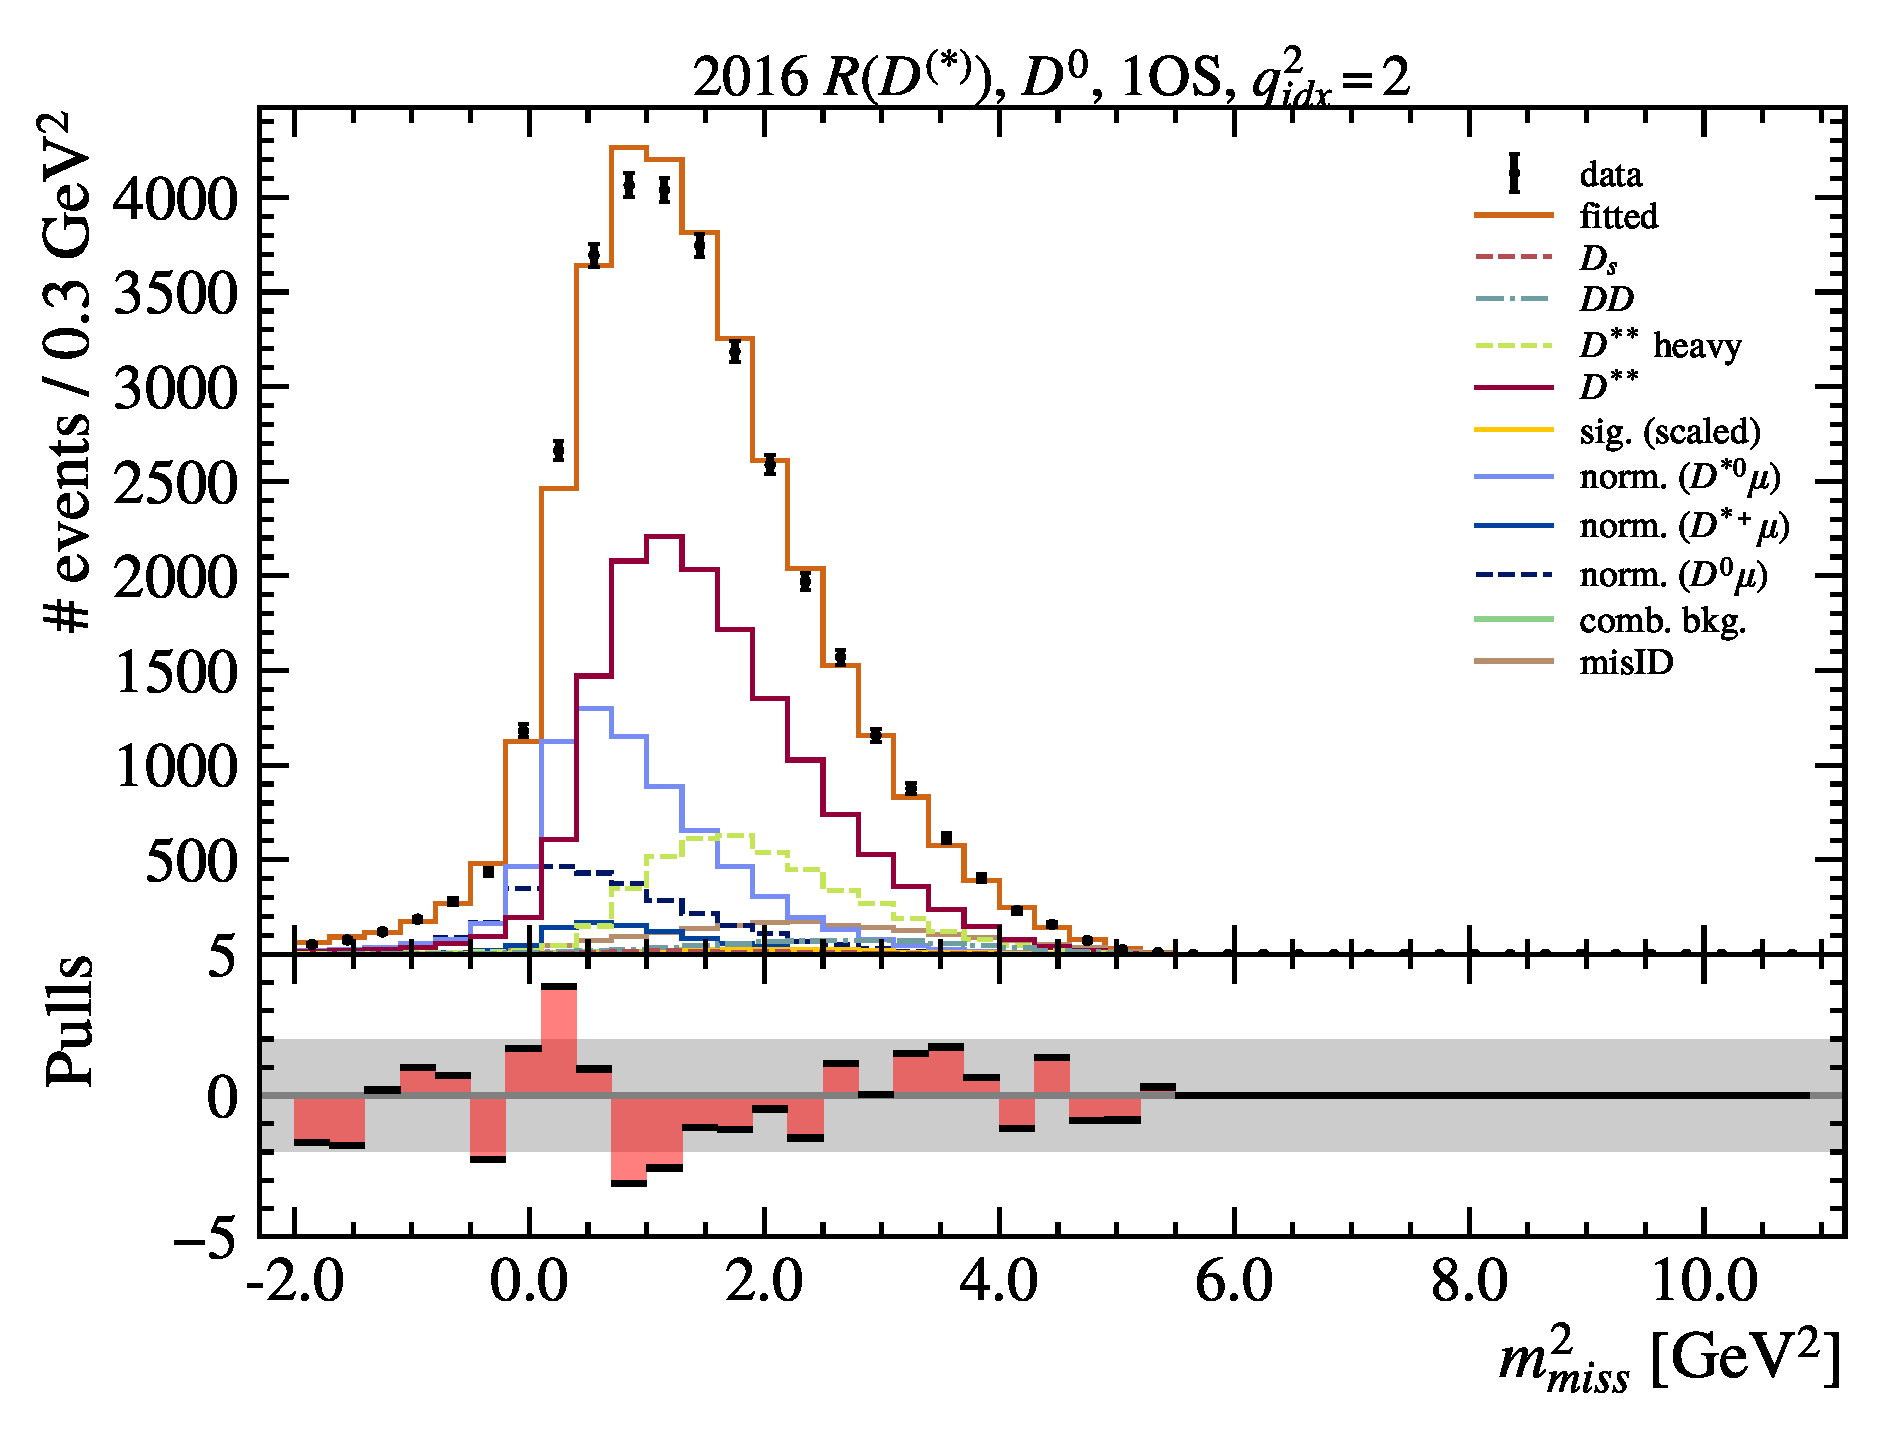
\includegraphics[width=0.24\textwidth]{./figs-fit-fit-results/ctrl-fit/lines_q2_slices/fit_result-lines_q2_idx2-D0-1os-mmiss2.pdf}
    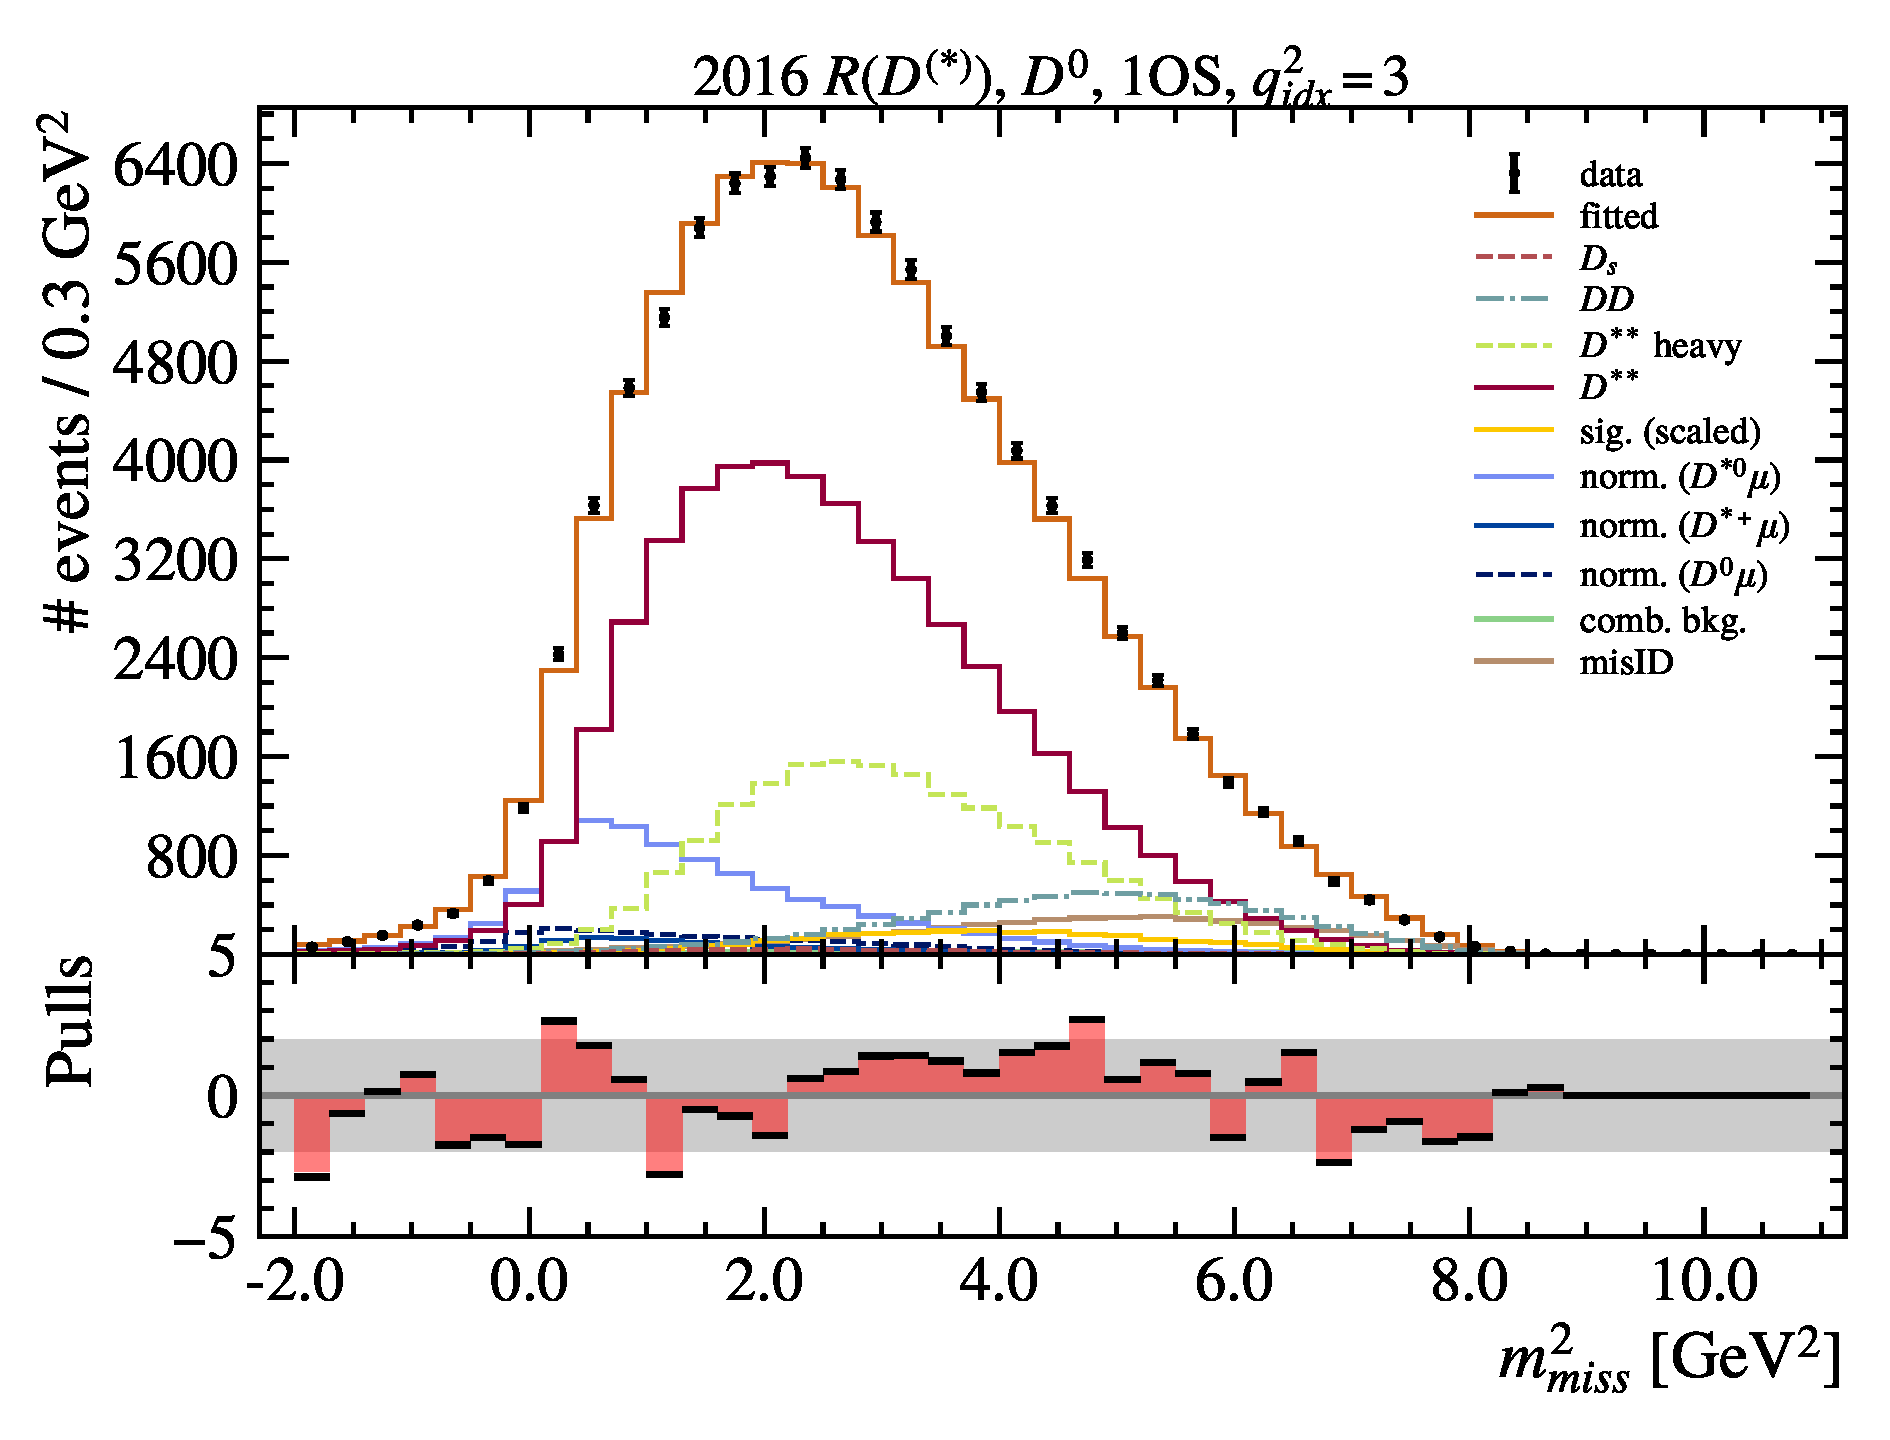
\includegraphics[width=0.24\textwidth]{./figs-fit-fit-results/ctrl-fit/lines_q2_slices/fit_result-lines_q2_idx3-D0-1os-mmiss2.pdf}
    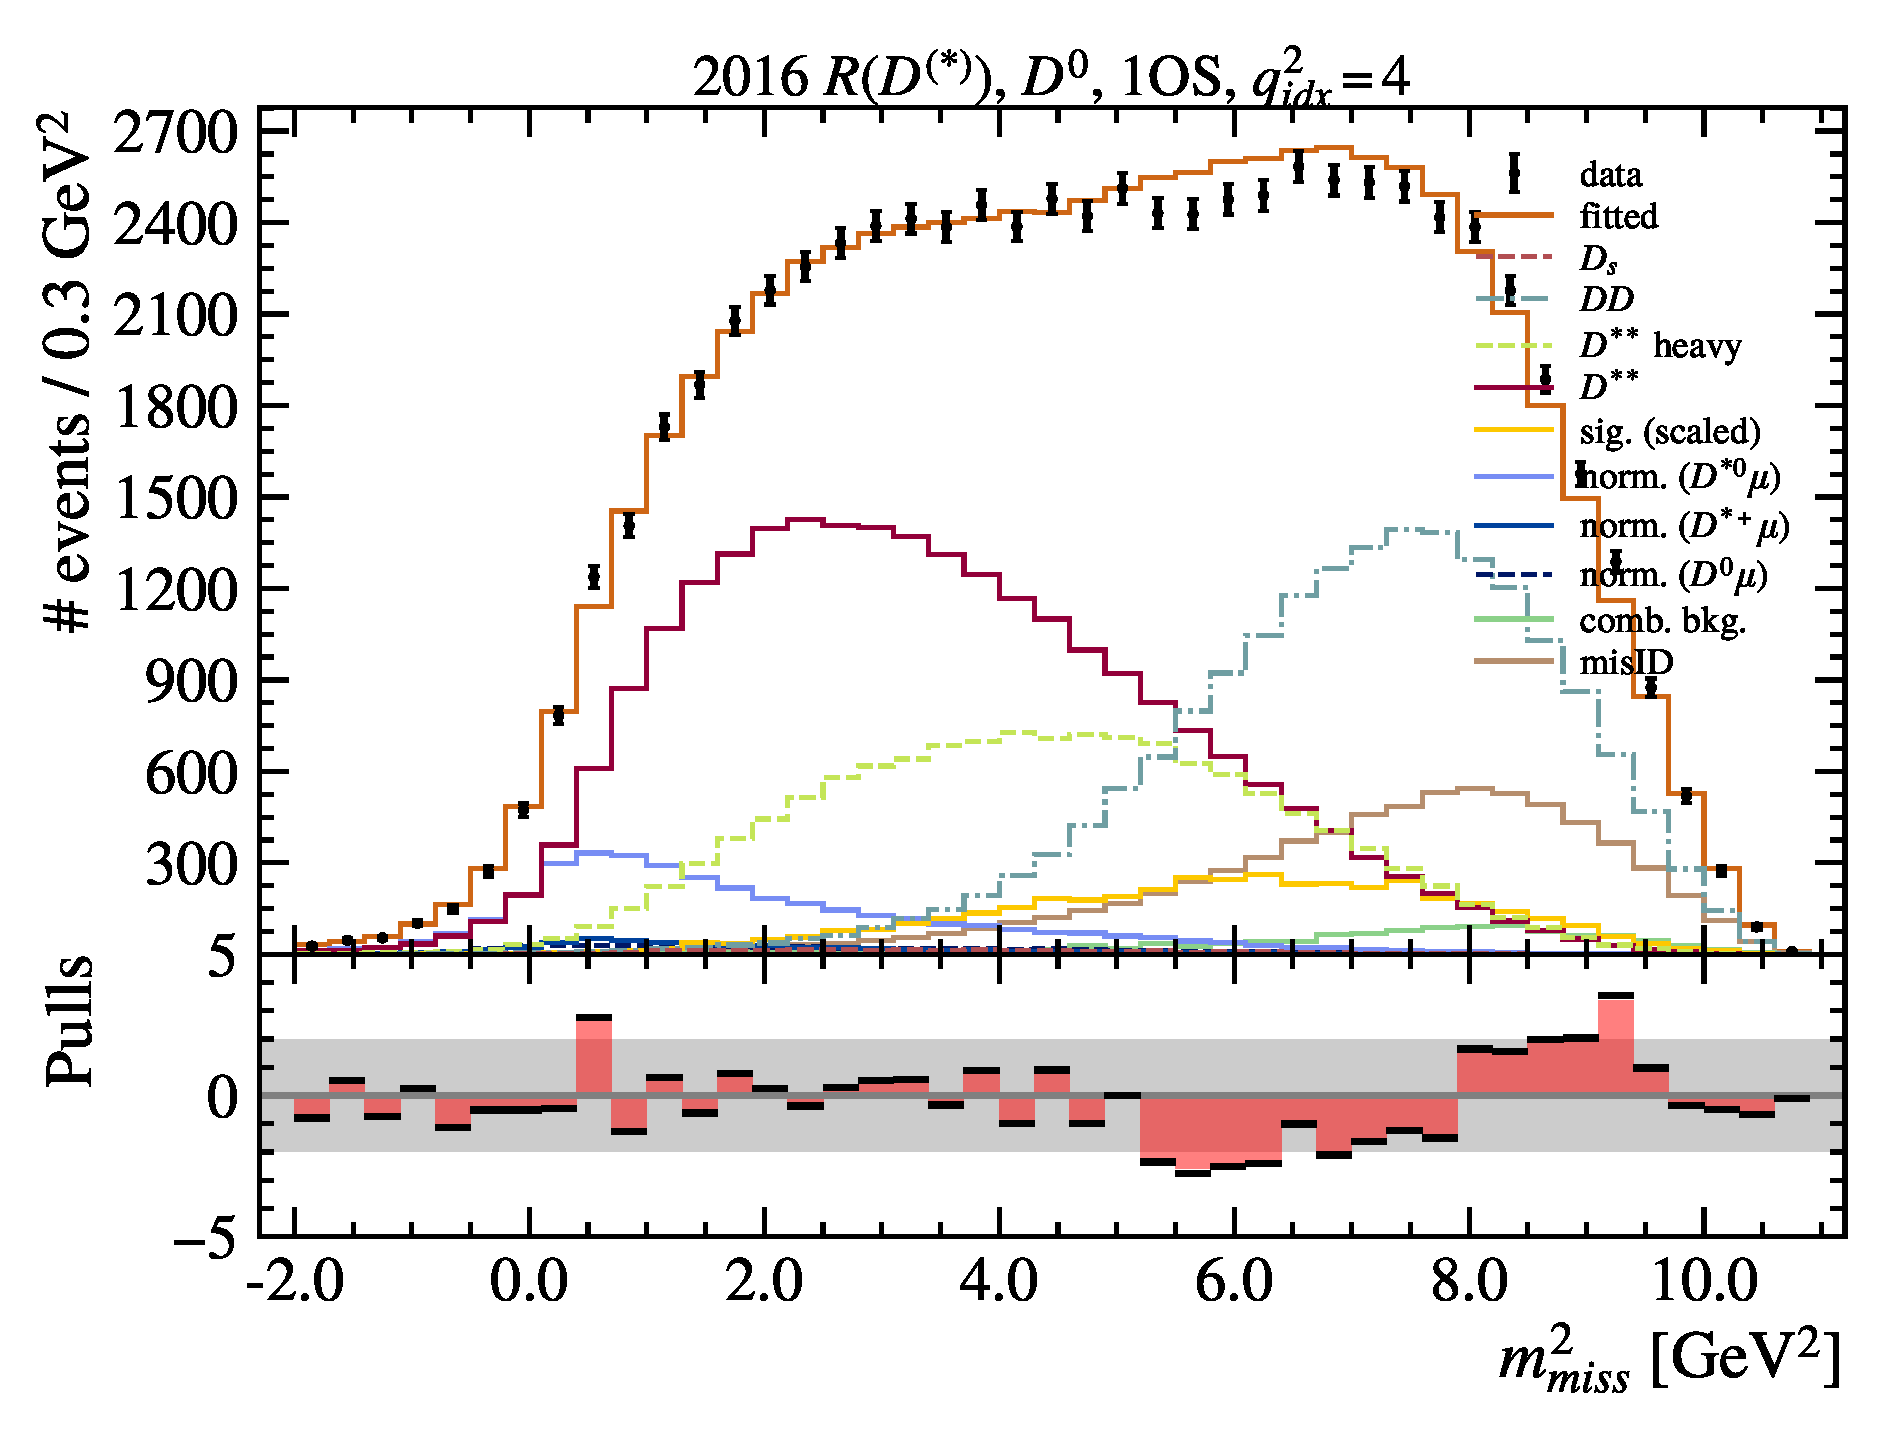
\includegraphics[width=0.24\textwidth]{./figs-fit-fit-results/ctrl-fit/lines_q2_slices/fit_result-lines_q2_idx4-D0-1os-mmiss2.pdf}

    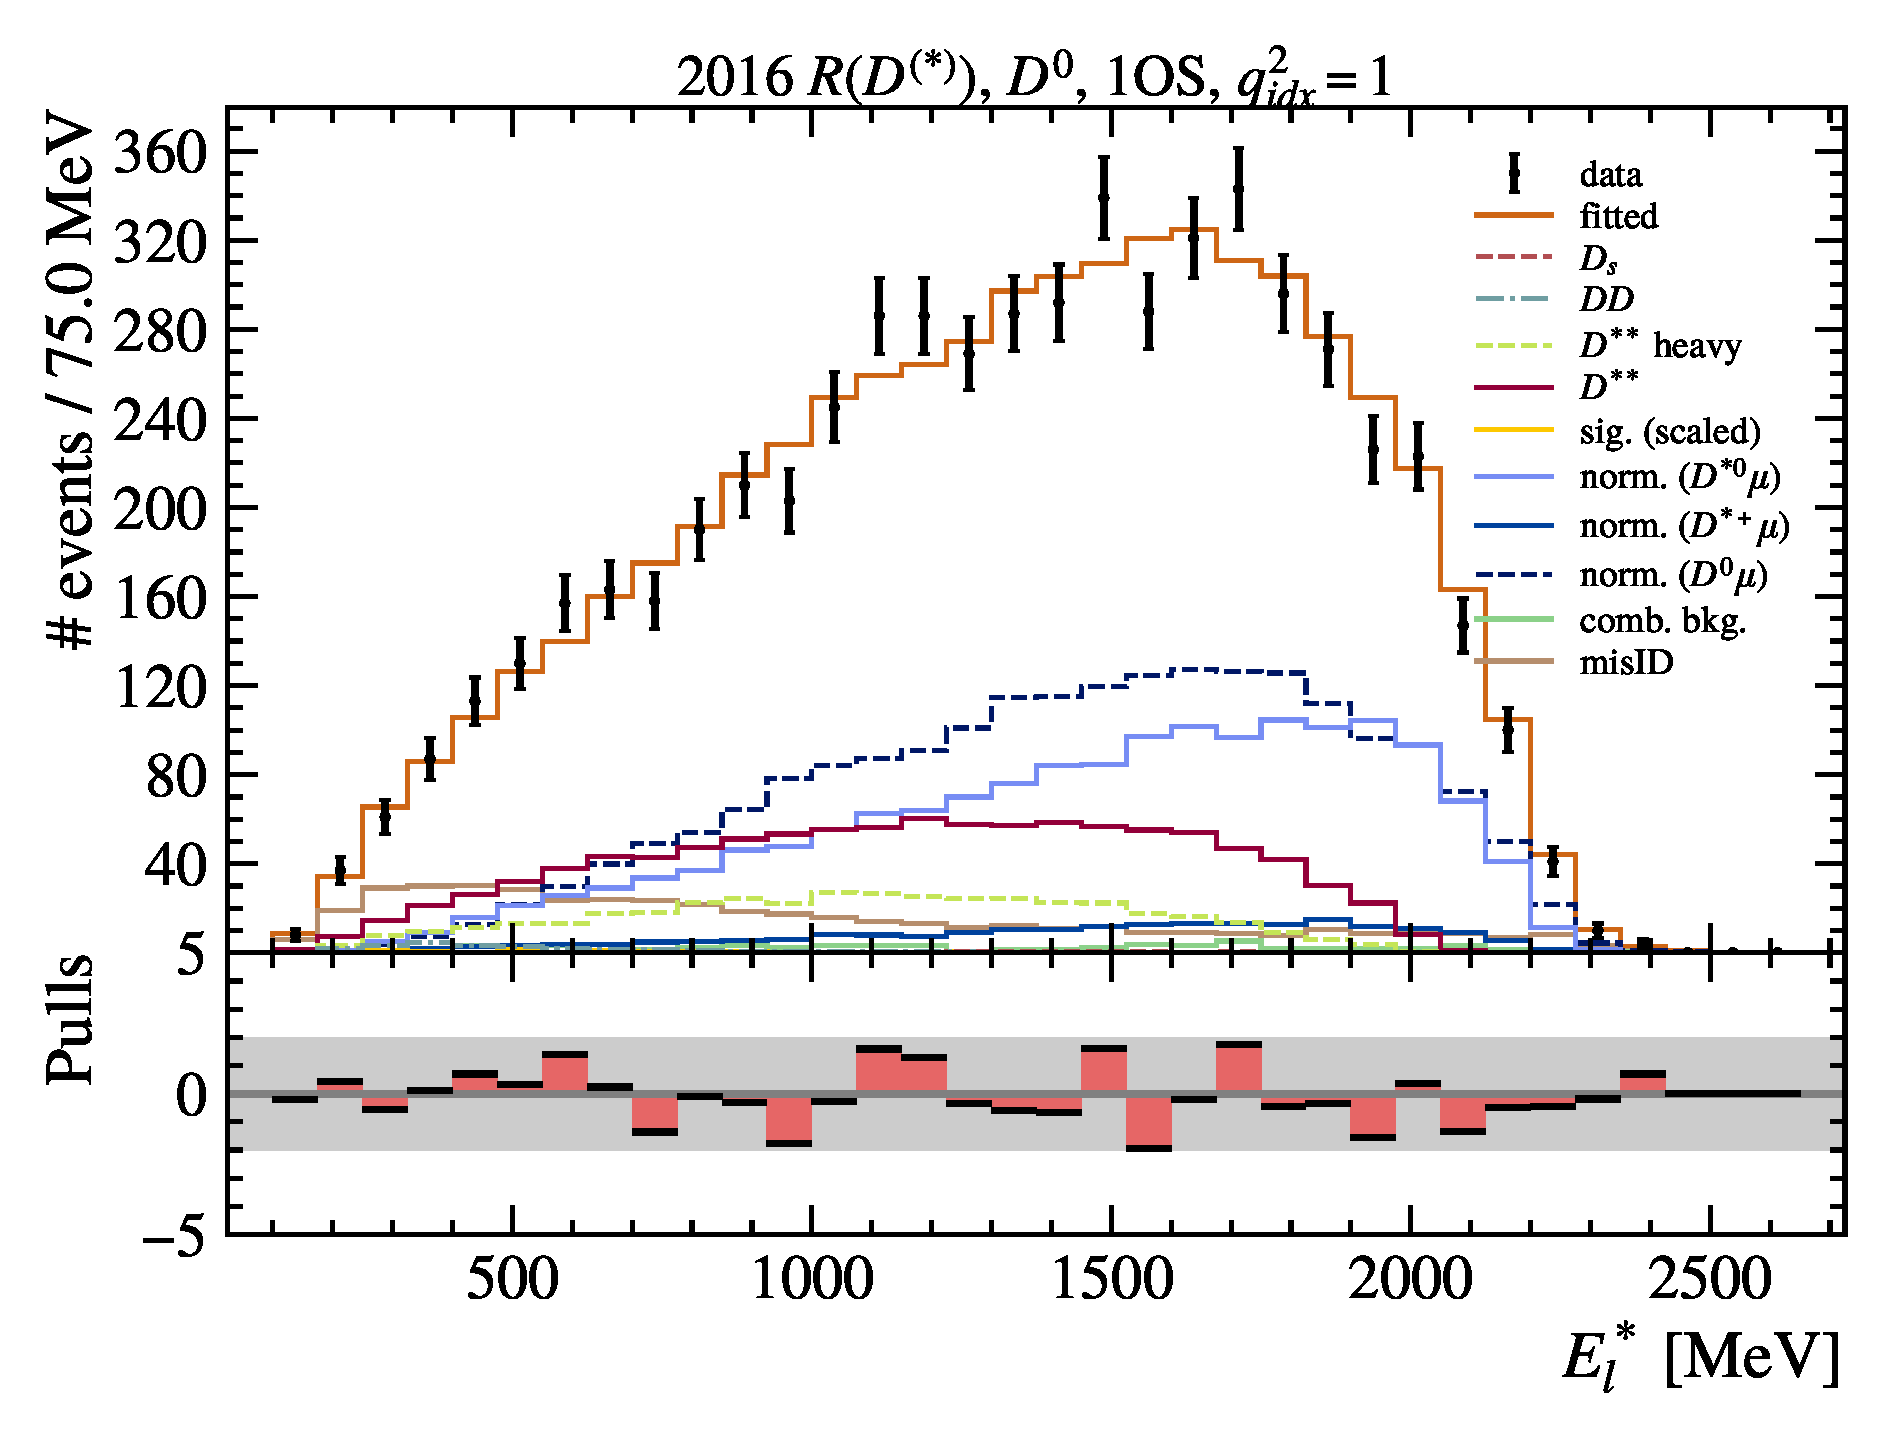
\includegraphics[width=0.24\textwidth]{./figs-fit-fit-results/ctrl-fit/lines_q2_slices/fit_result-lines_q2_idx1-D0-1os-el.pdf}
    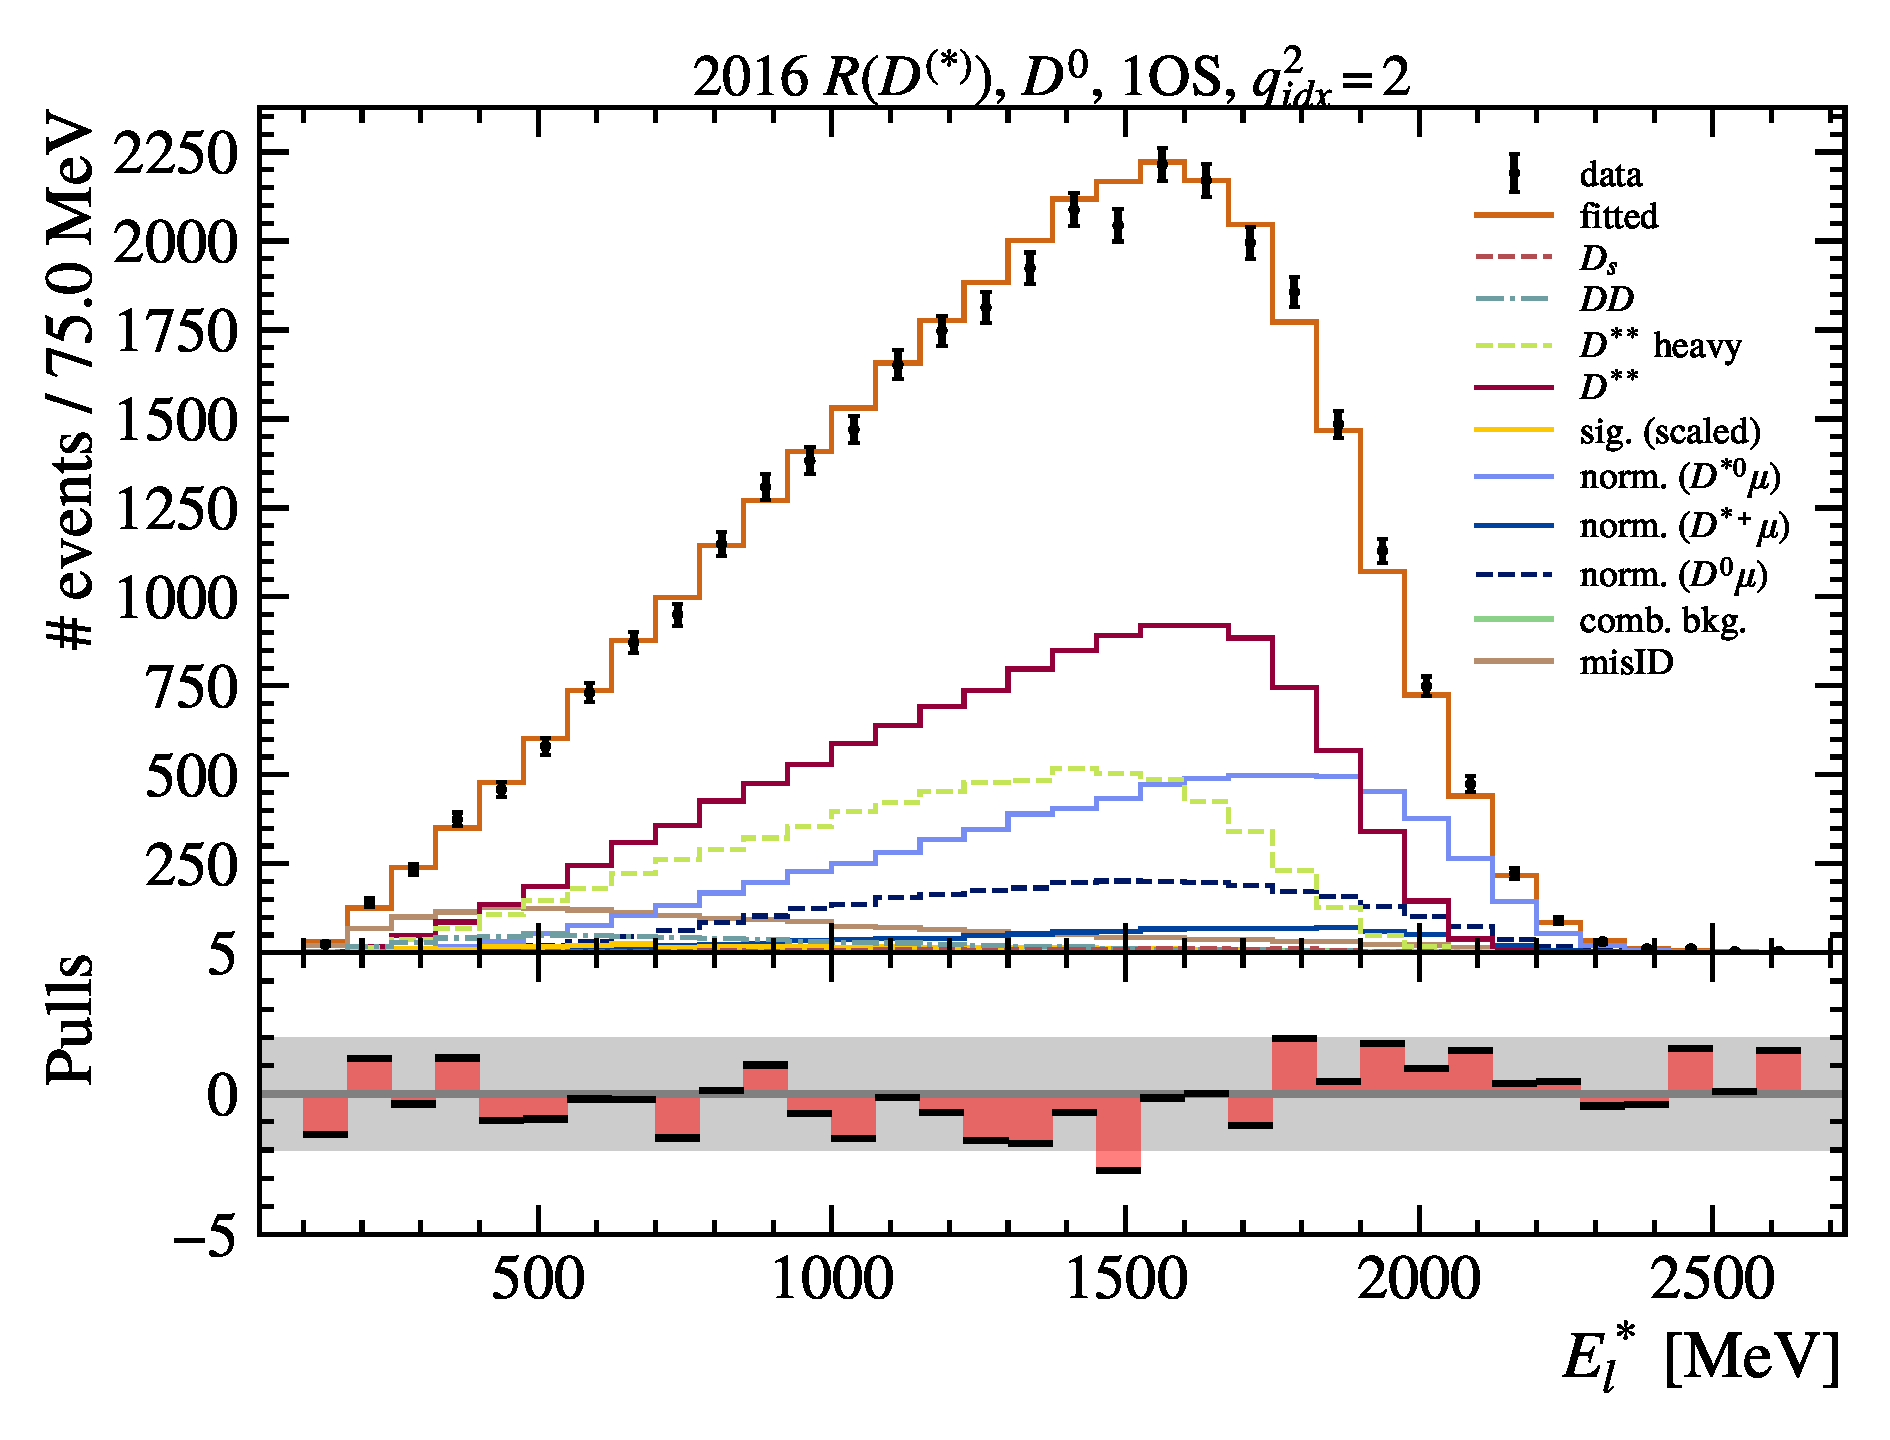
\includegraphics[width=0.24\textwidth]{./figs-fit-fit-results/ctrl-fit/lines_q2_slices/fit_result-lines_q2_idx2-D0-1os-el.pdf}
    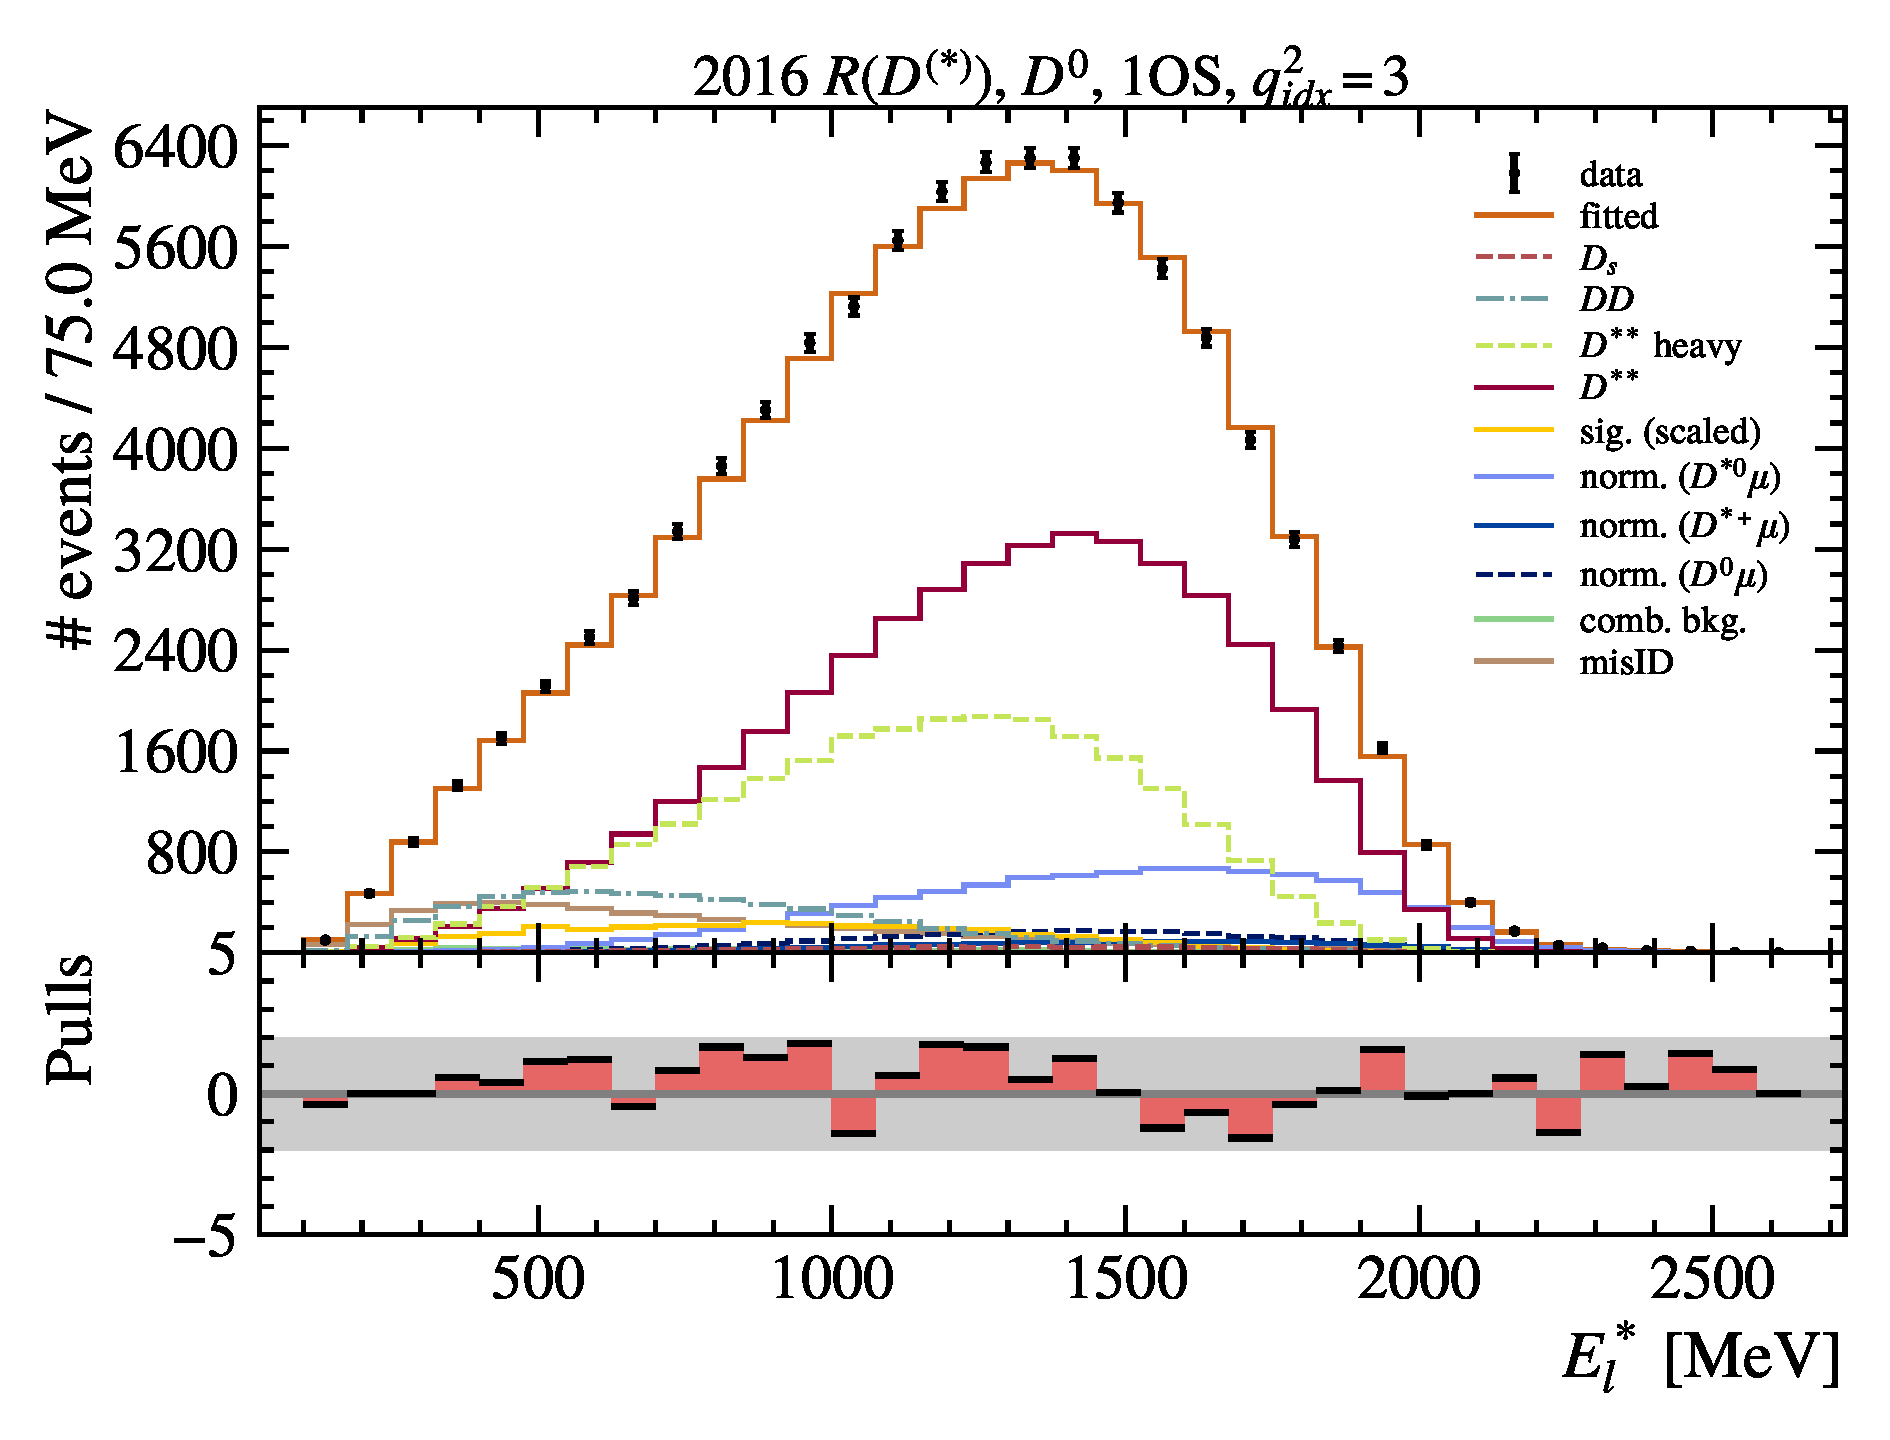
\includegraphics[width=0.24\textwidth]{./figs-fit-fit-results/ctrl-fit/lines_q2_slices/fit_result-lines_q2_idx3-D0-1os-el.pdf}
    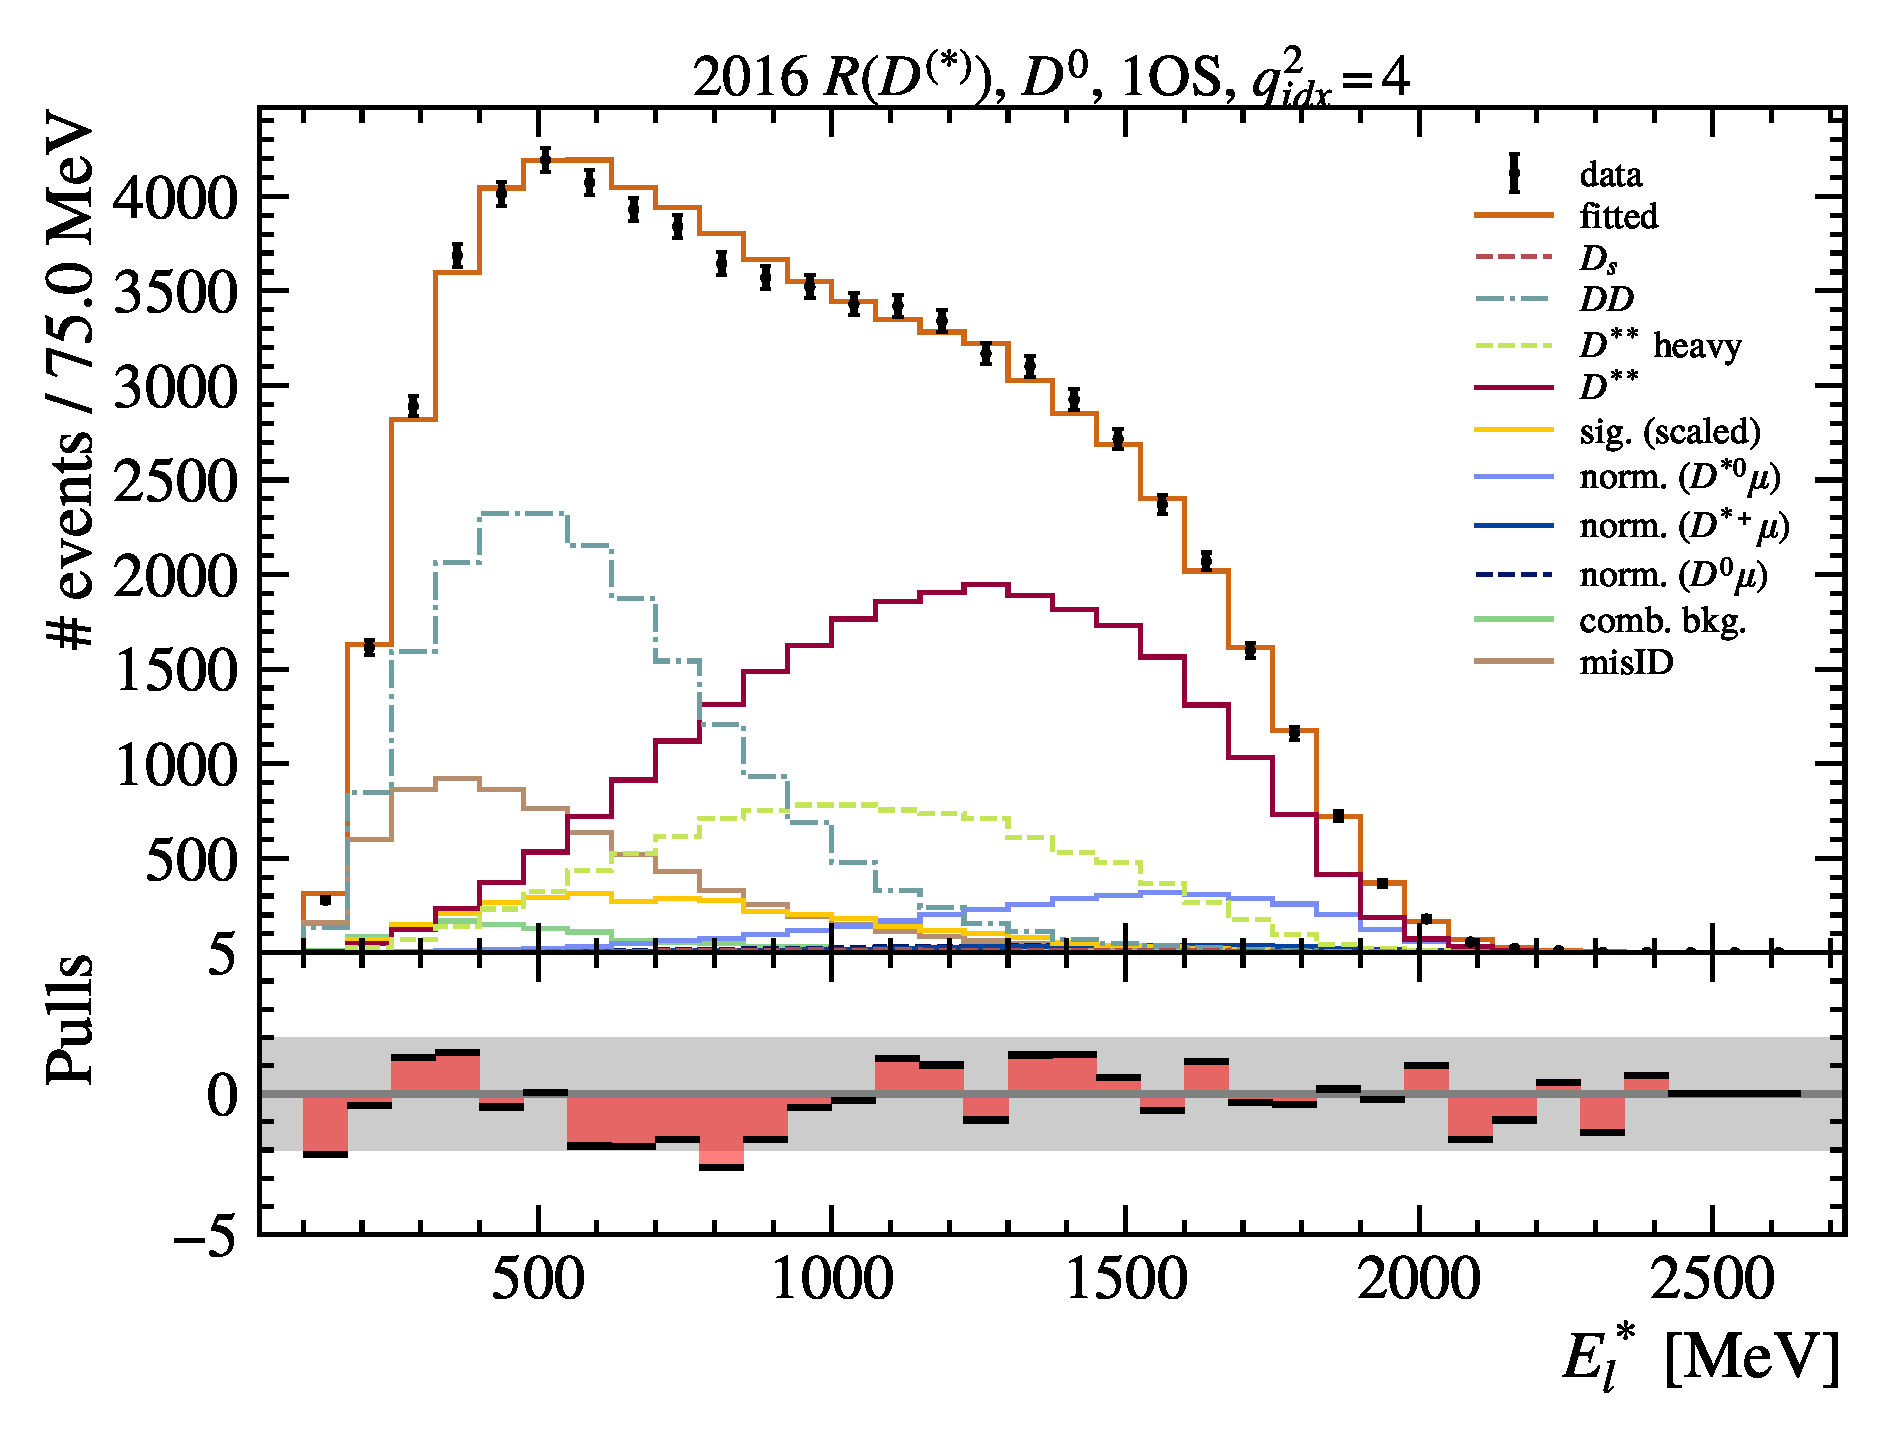
\includegraphics[width=0.24\textwidth]{./figs-fit-fit-results/ctrl-fit/lines_q2_slices/fit_result-lines_q2_idx4-D0-1os-el.pdf}

    \caption{Control fit for 1OS sample, \Dz channel.}
    \label{fig:ctrl-1os-d0}
\end{figure}

\begin{figure}[!htb]
    \centering
    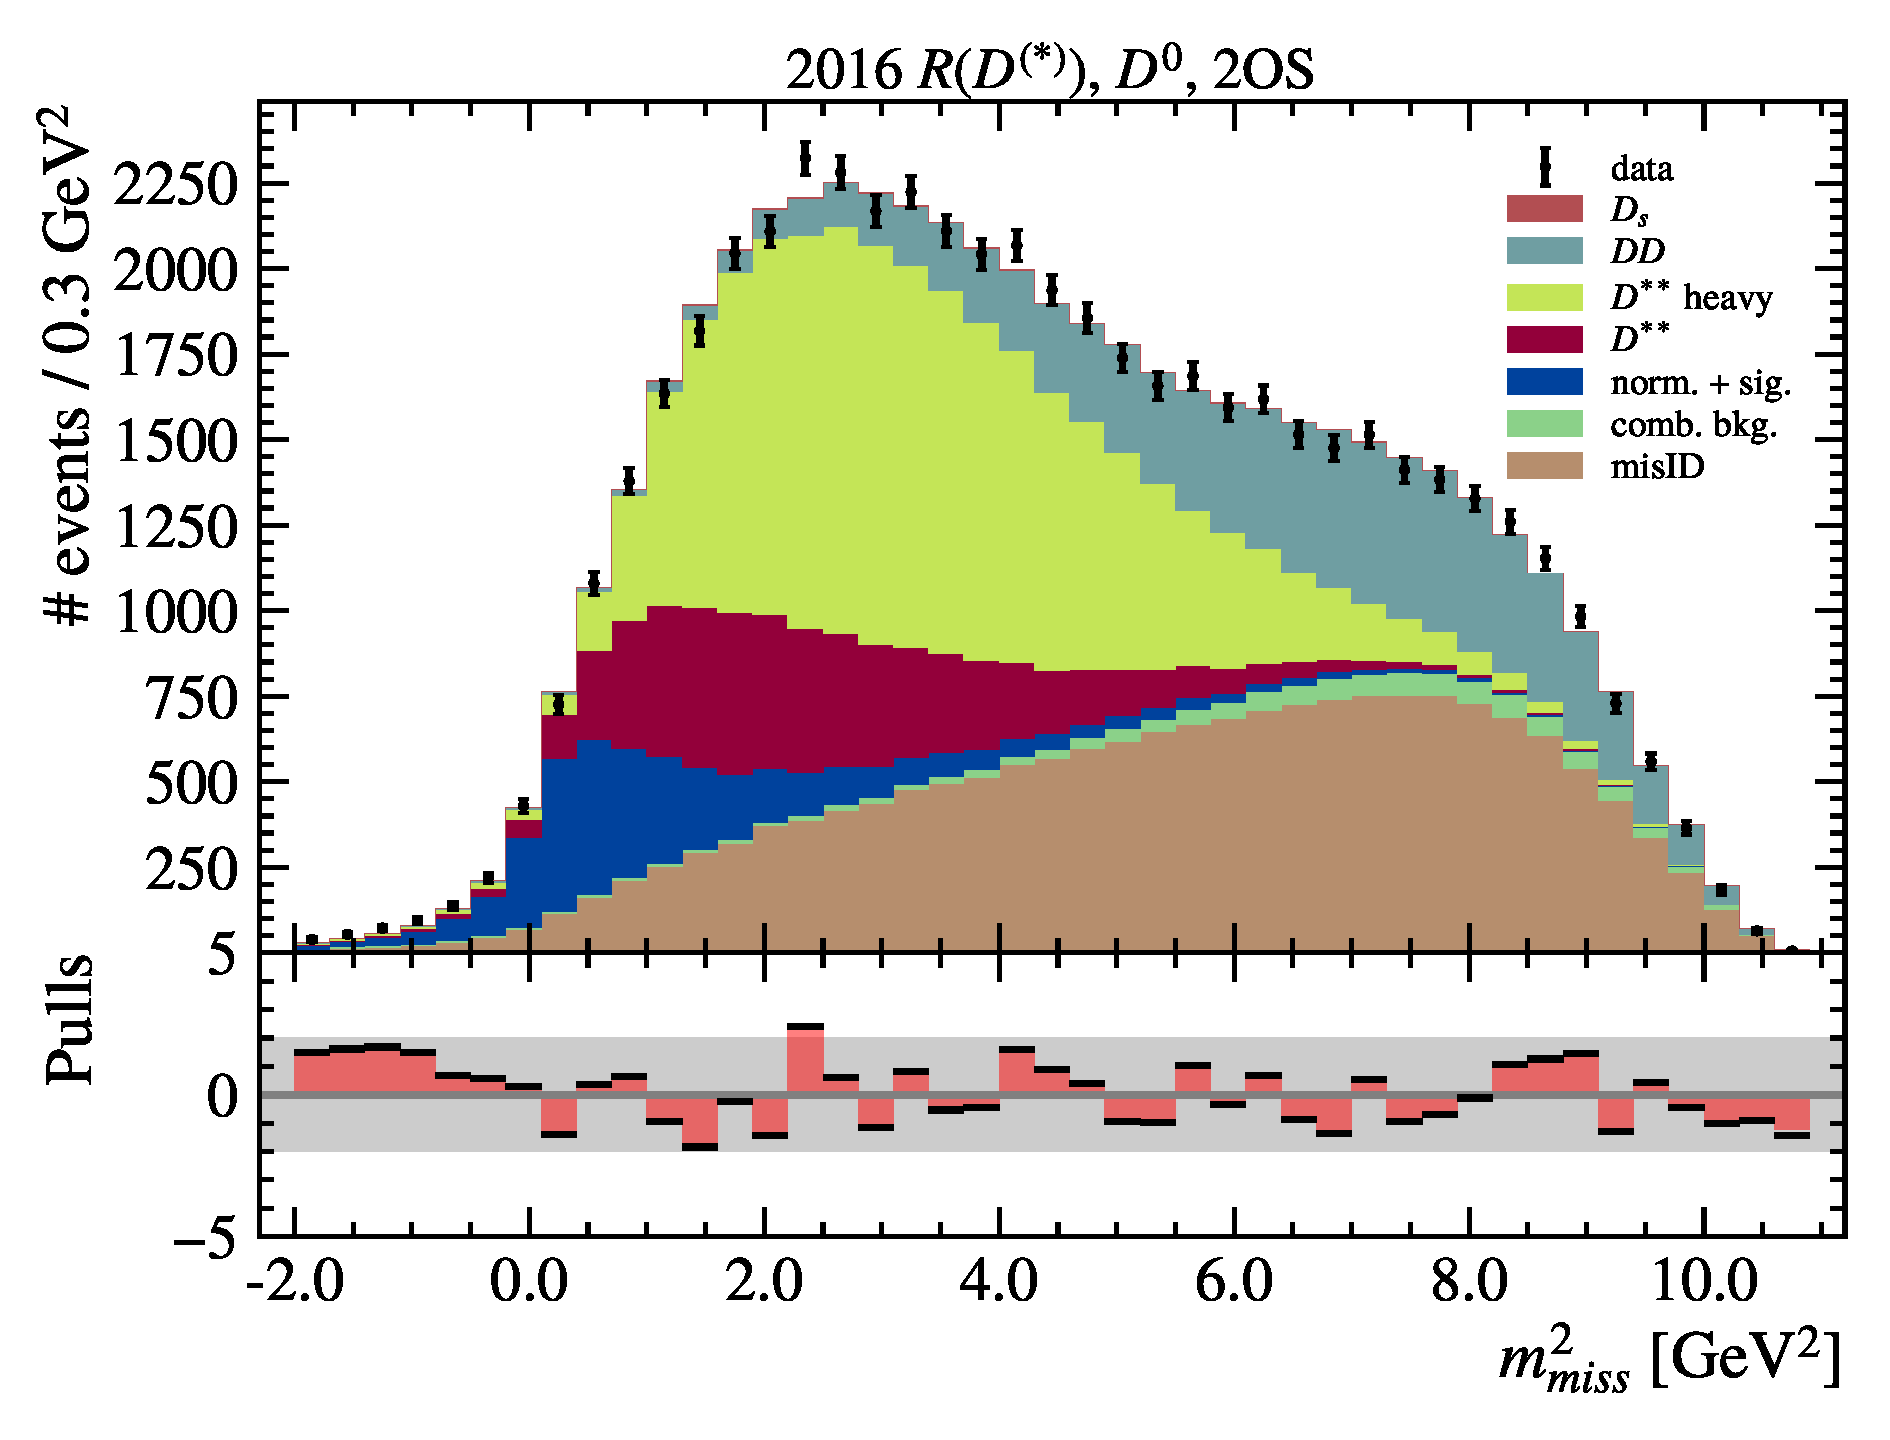
\includegraphics[width=0.32\textwidth]{./figs-fit-fit-results/ctrl-fit/stacked/fit_result-stacked-D0-2os-mmiss2.pdf}
    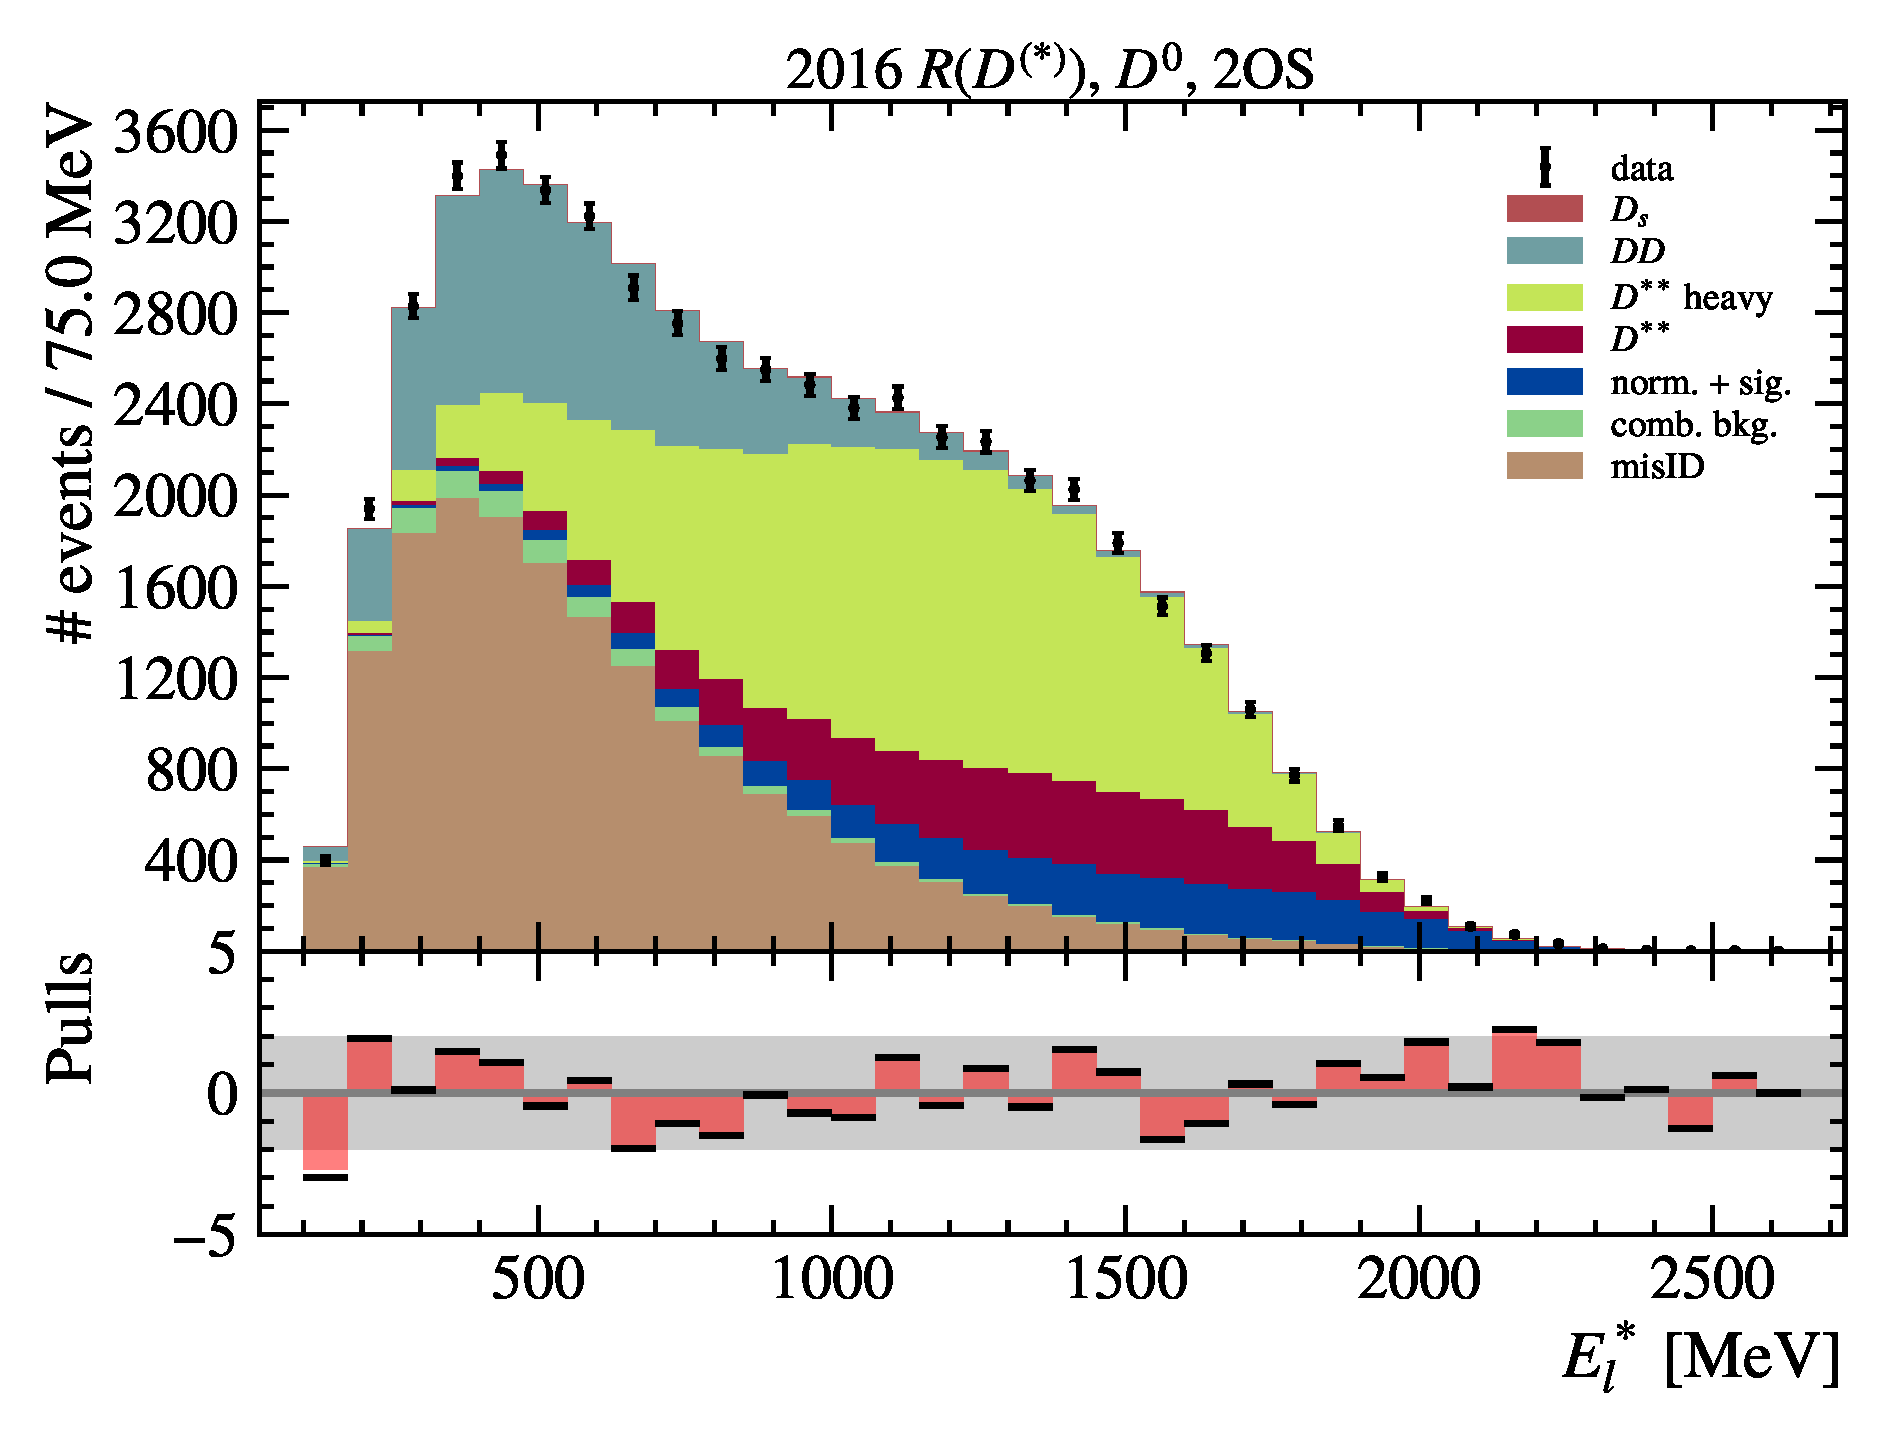
\includegraphics[width=0.32\textwidth]{./figs-fit-fit-results/ctrl-fit/stacked/fit_result-stacked-D0-2os-el.pdf}
    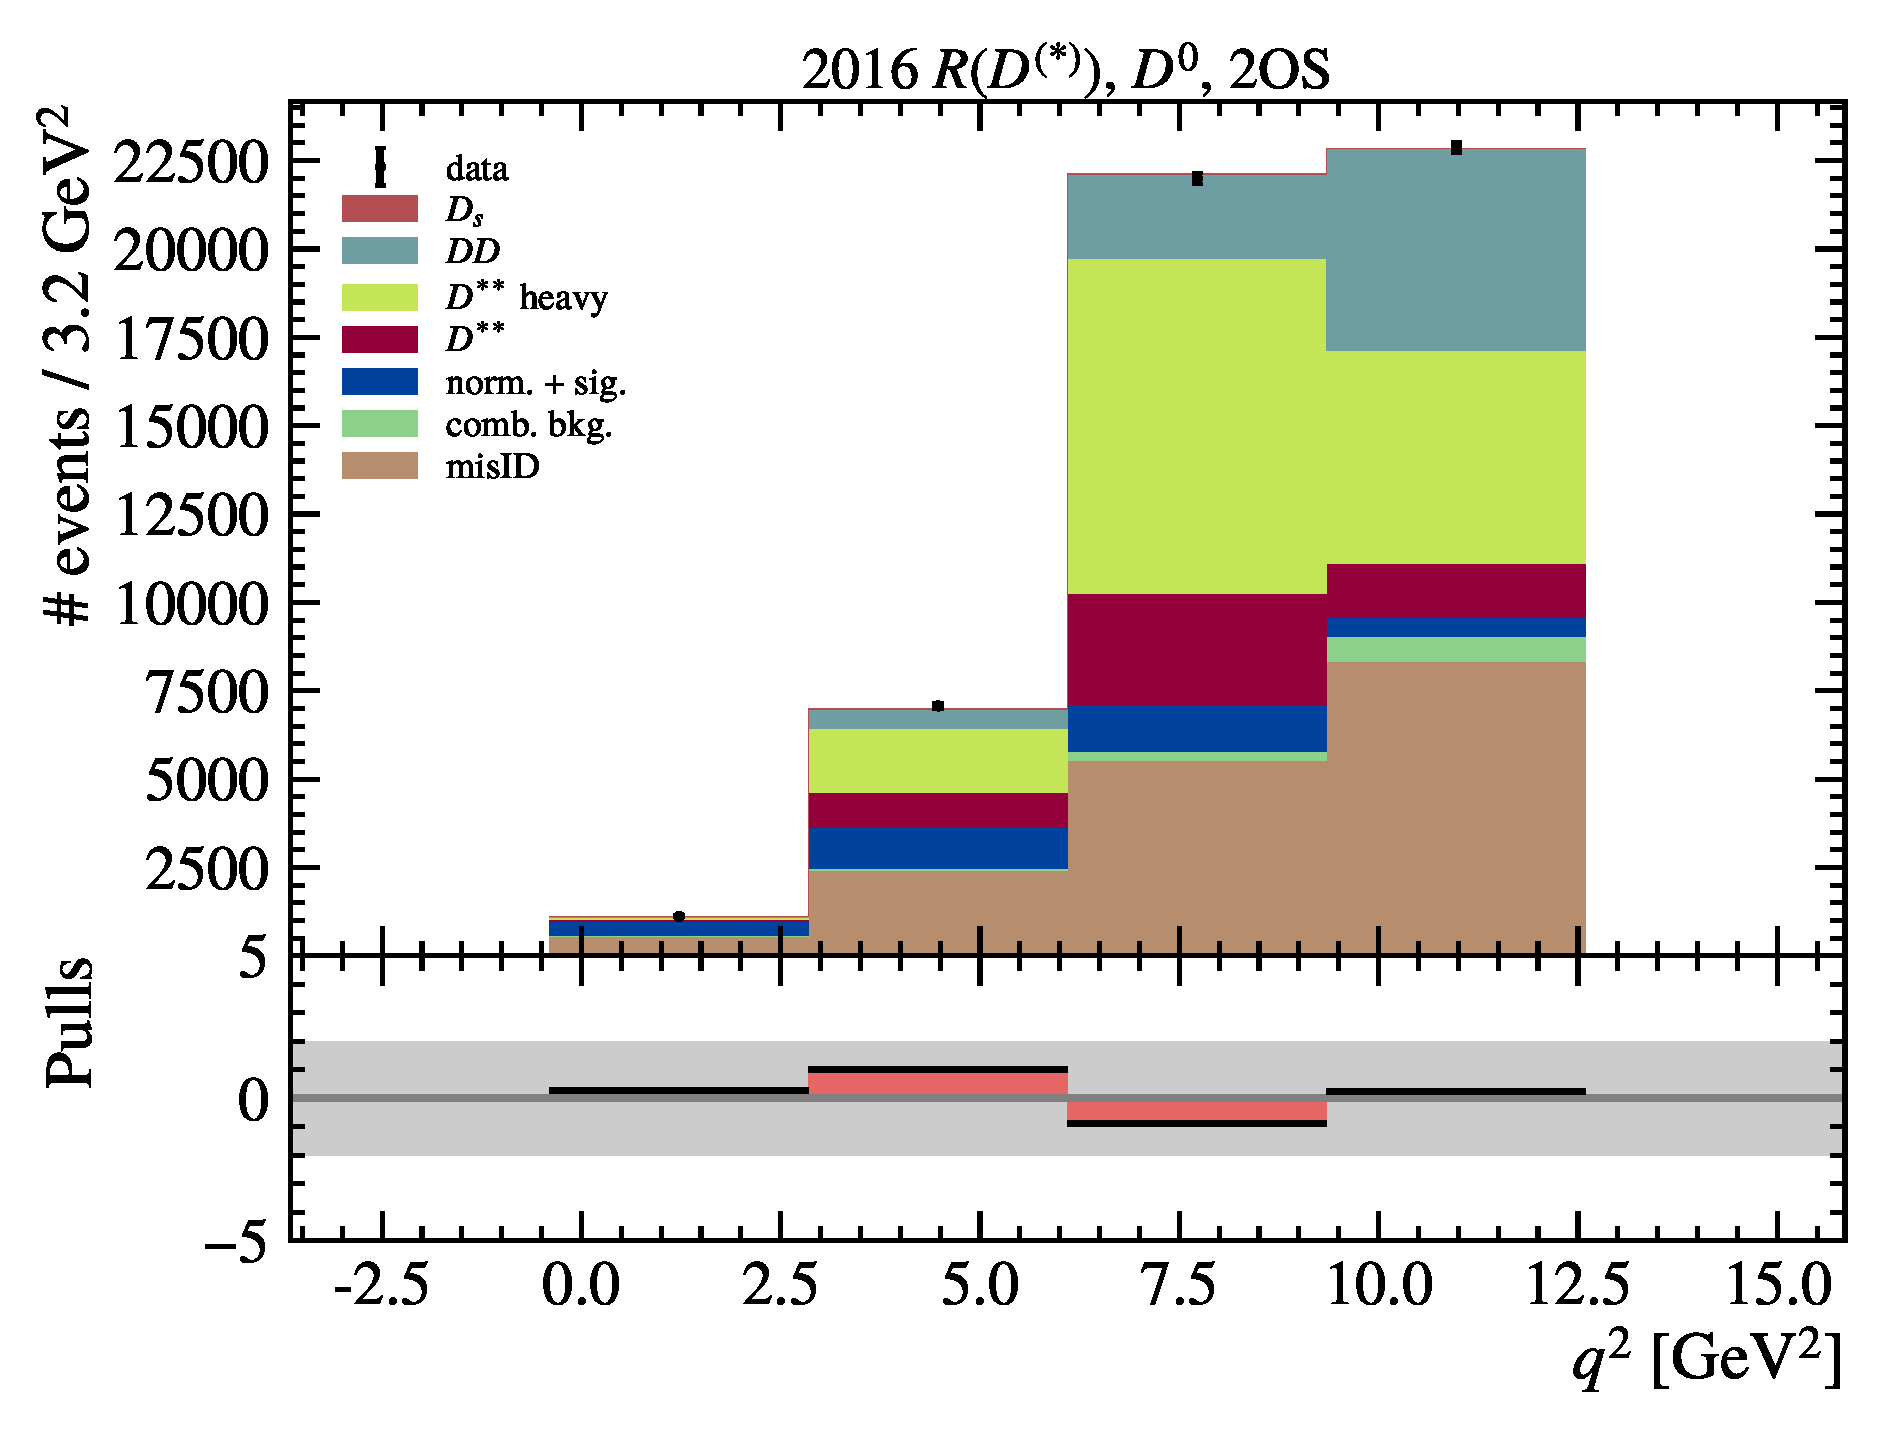
\includegraphics[width=0.32\textwidth]{./figs-fit-fit-results/ctrl-fit/stacked/fit_result-stacked-D0-2os-q2.pdf}

    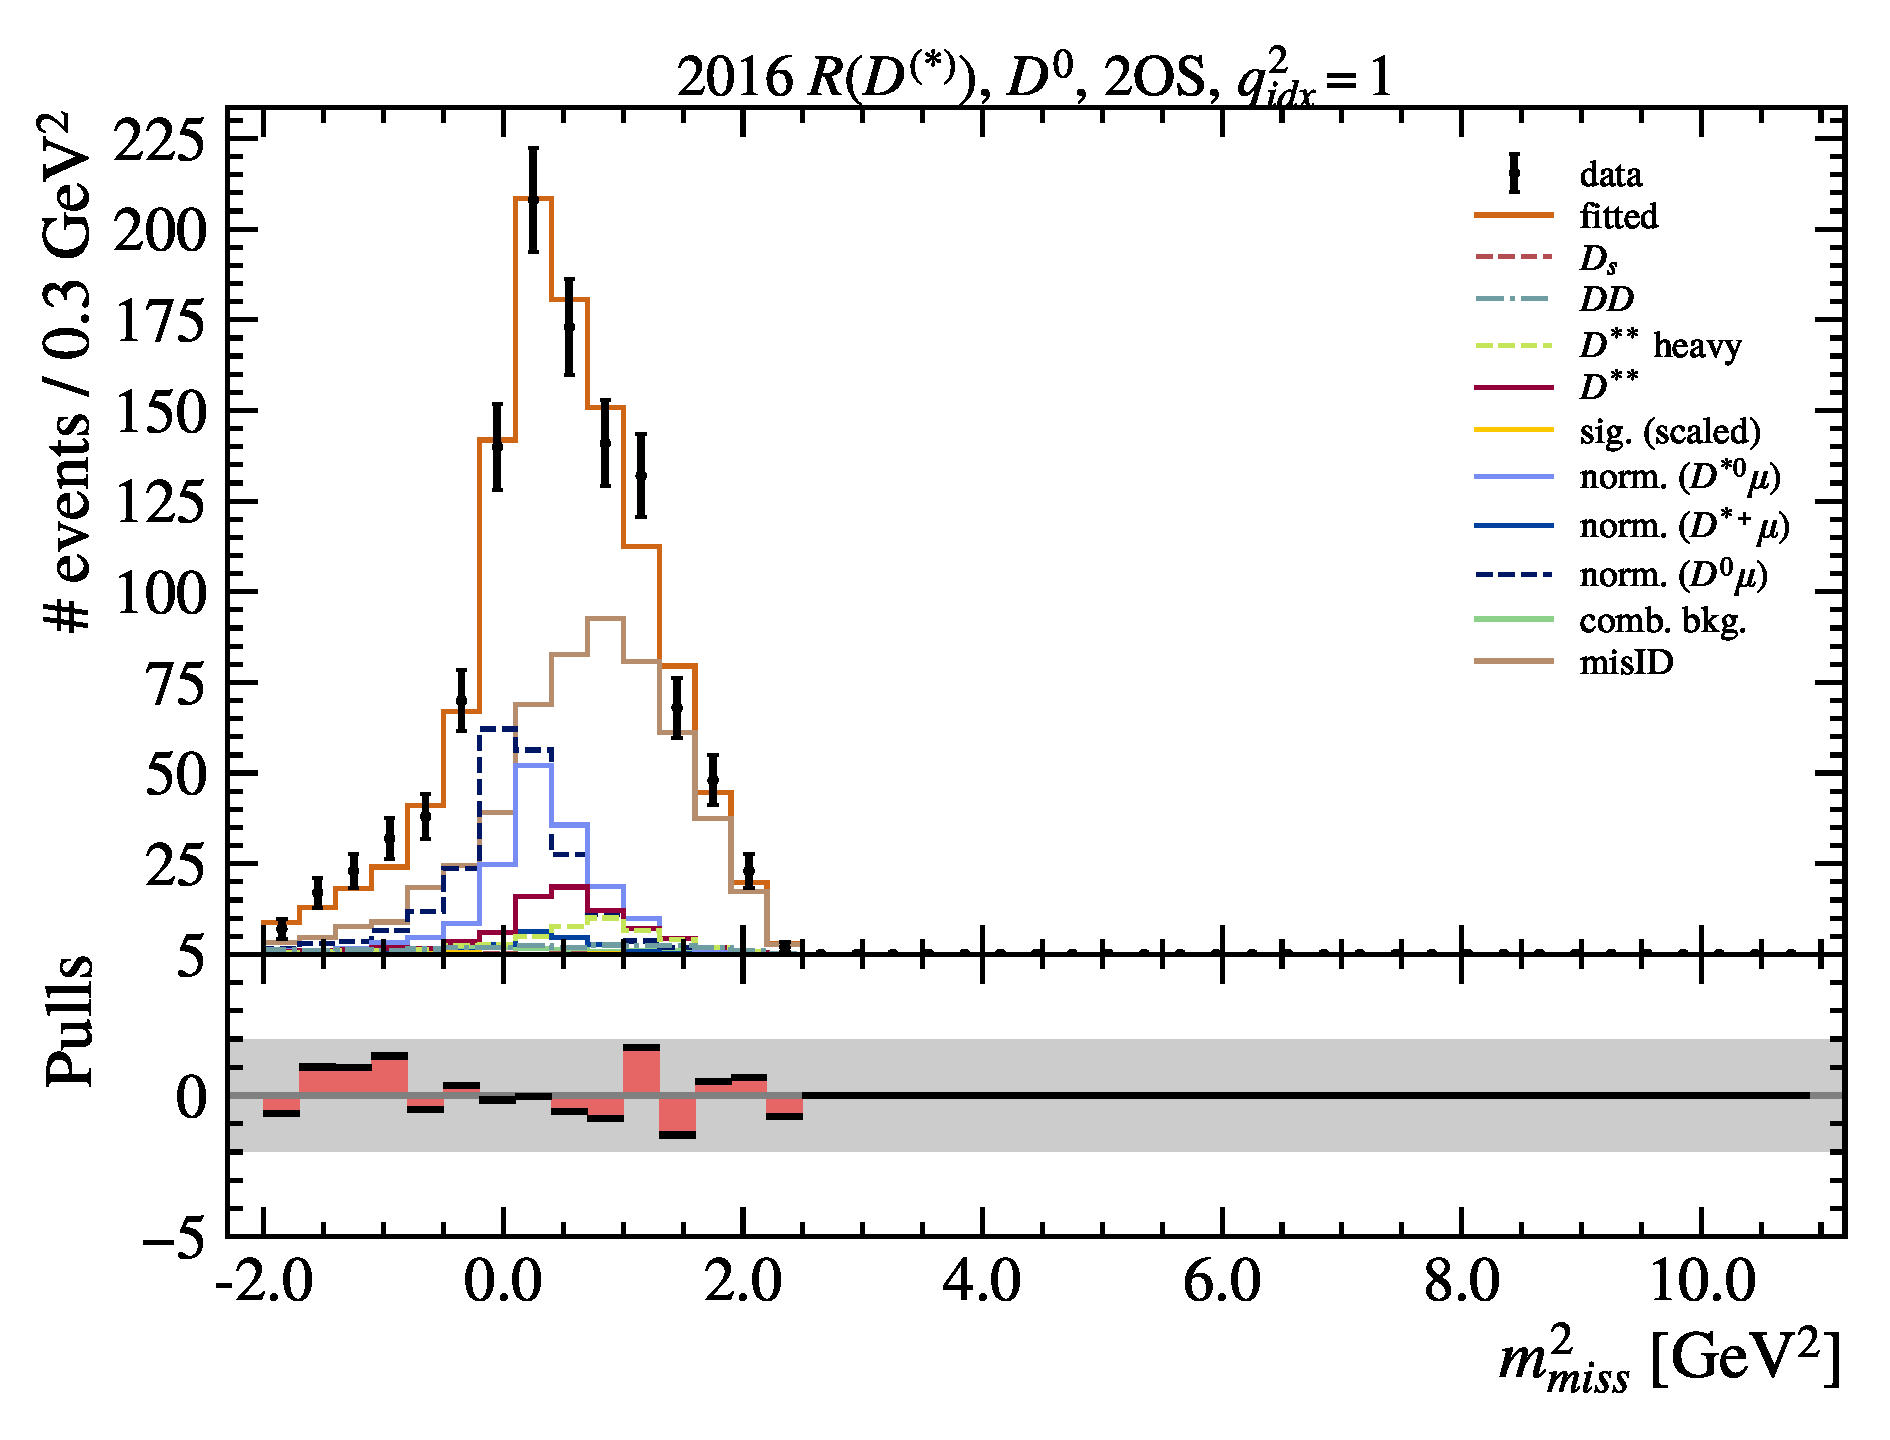
\includegraphics[width=0.24\textwidth]{./figs-fit-fit-results/ctrl-fit/lines_q2_slices/fit_result-lines_q2_idx1-D0-2os-mmiss2.pdf}
    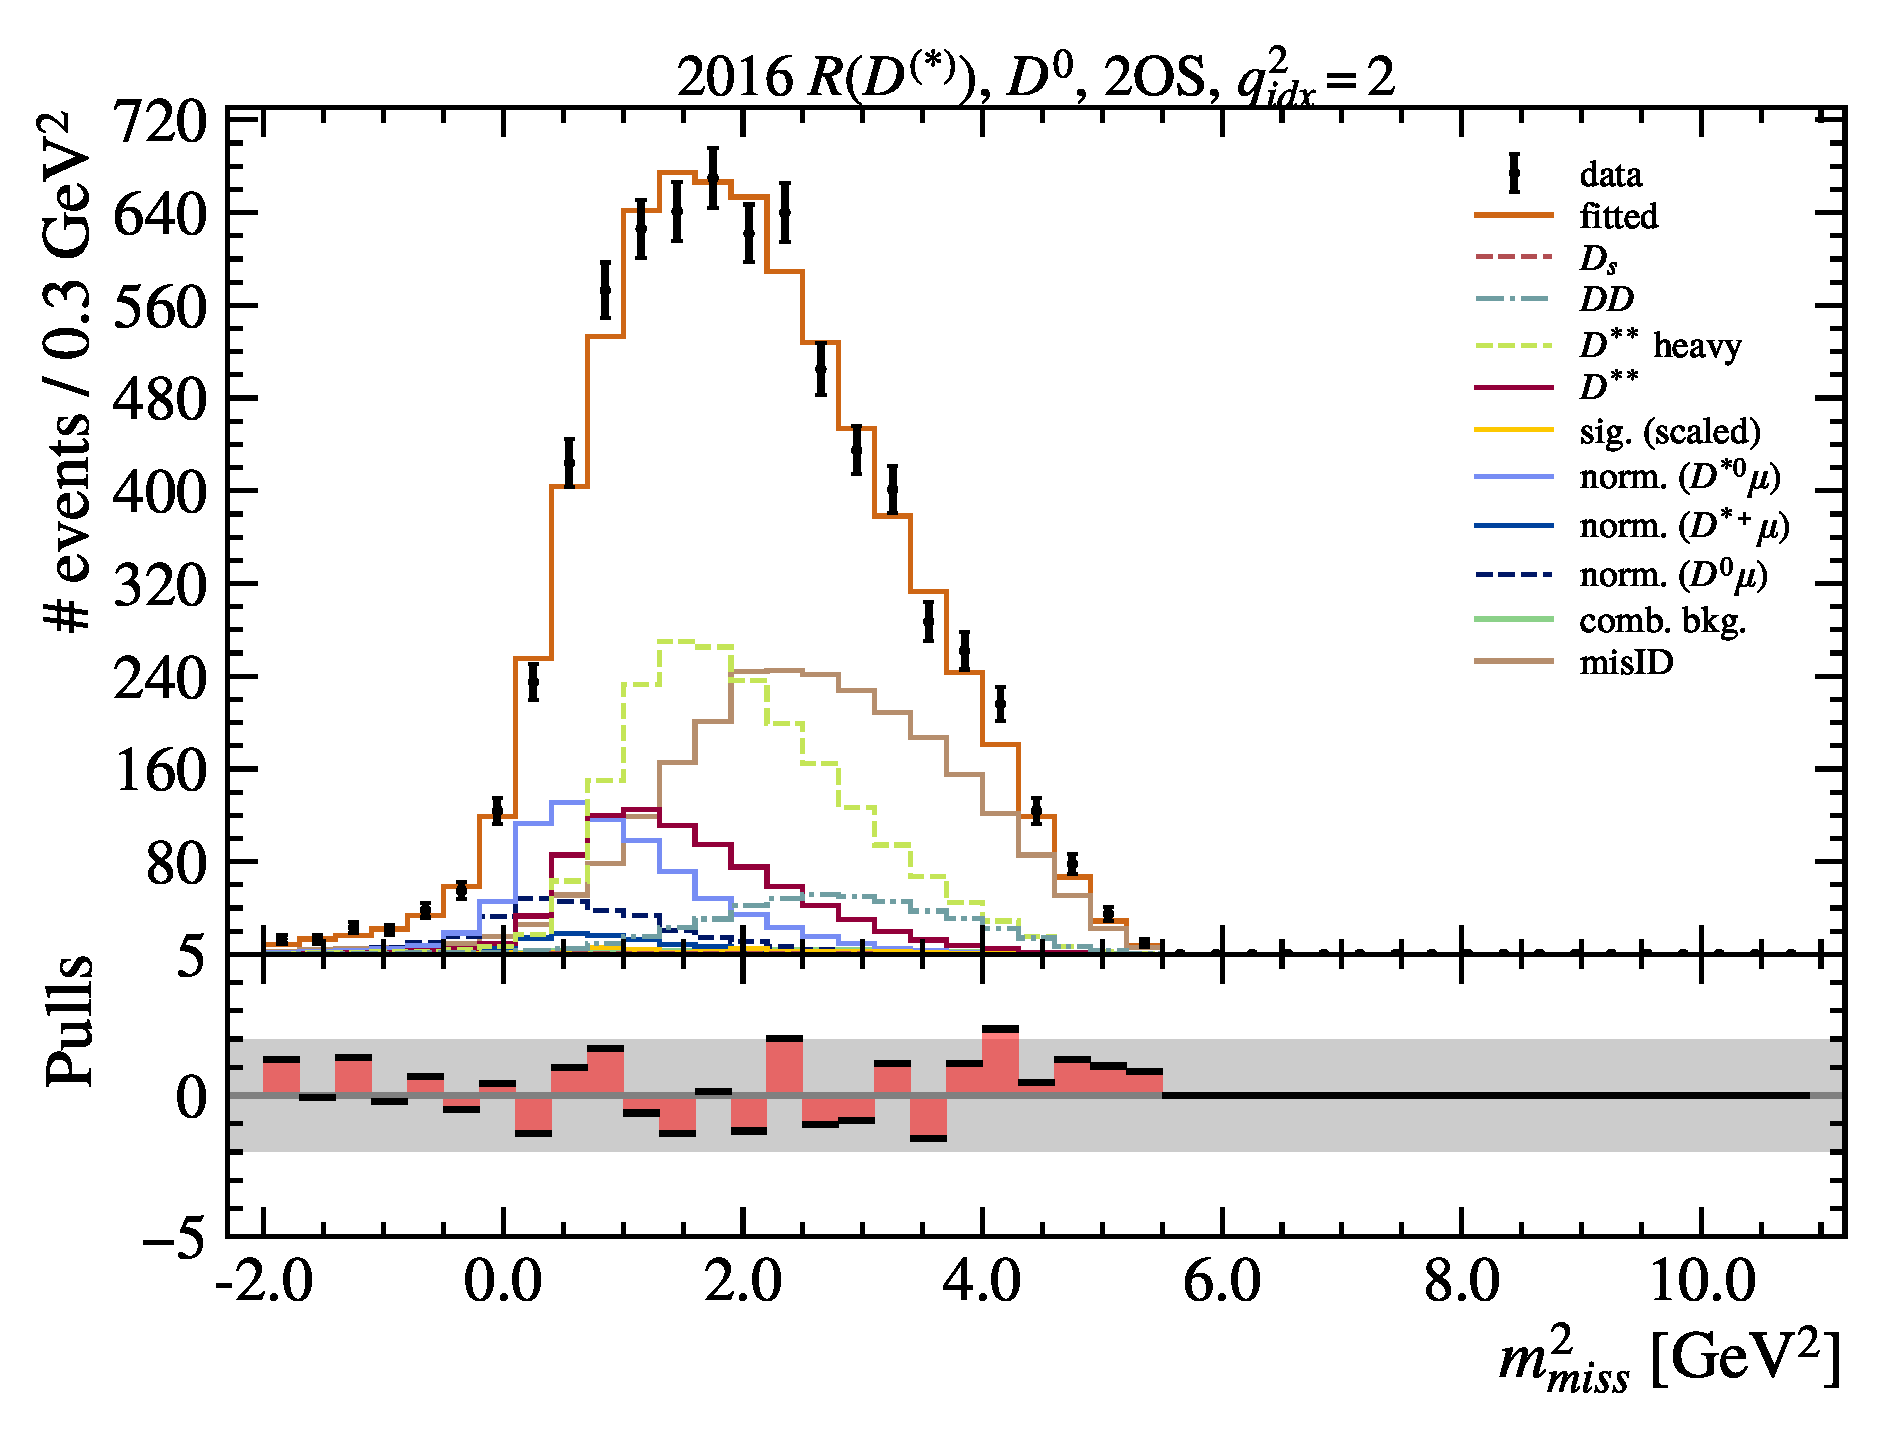
\includegraphics[width=0.24\textwidth]{./figs-fit-fit-results/ctrl-fit/lines_q2_slices/fit_result-lines_q2_idx2-D0-2os-mmiss2.pdf}
    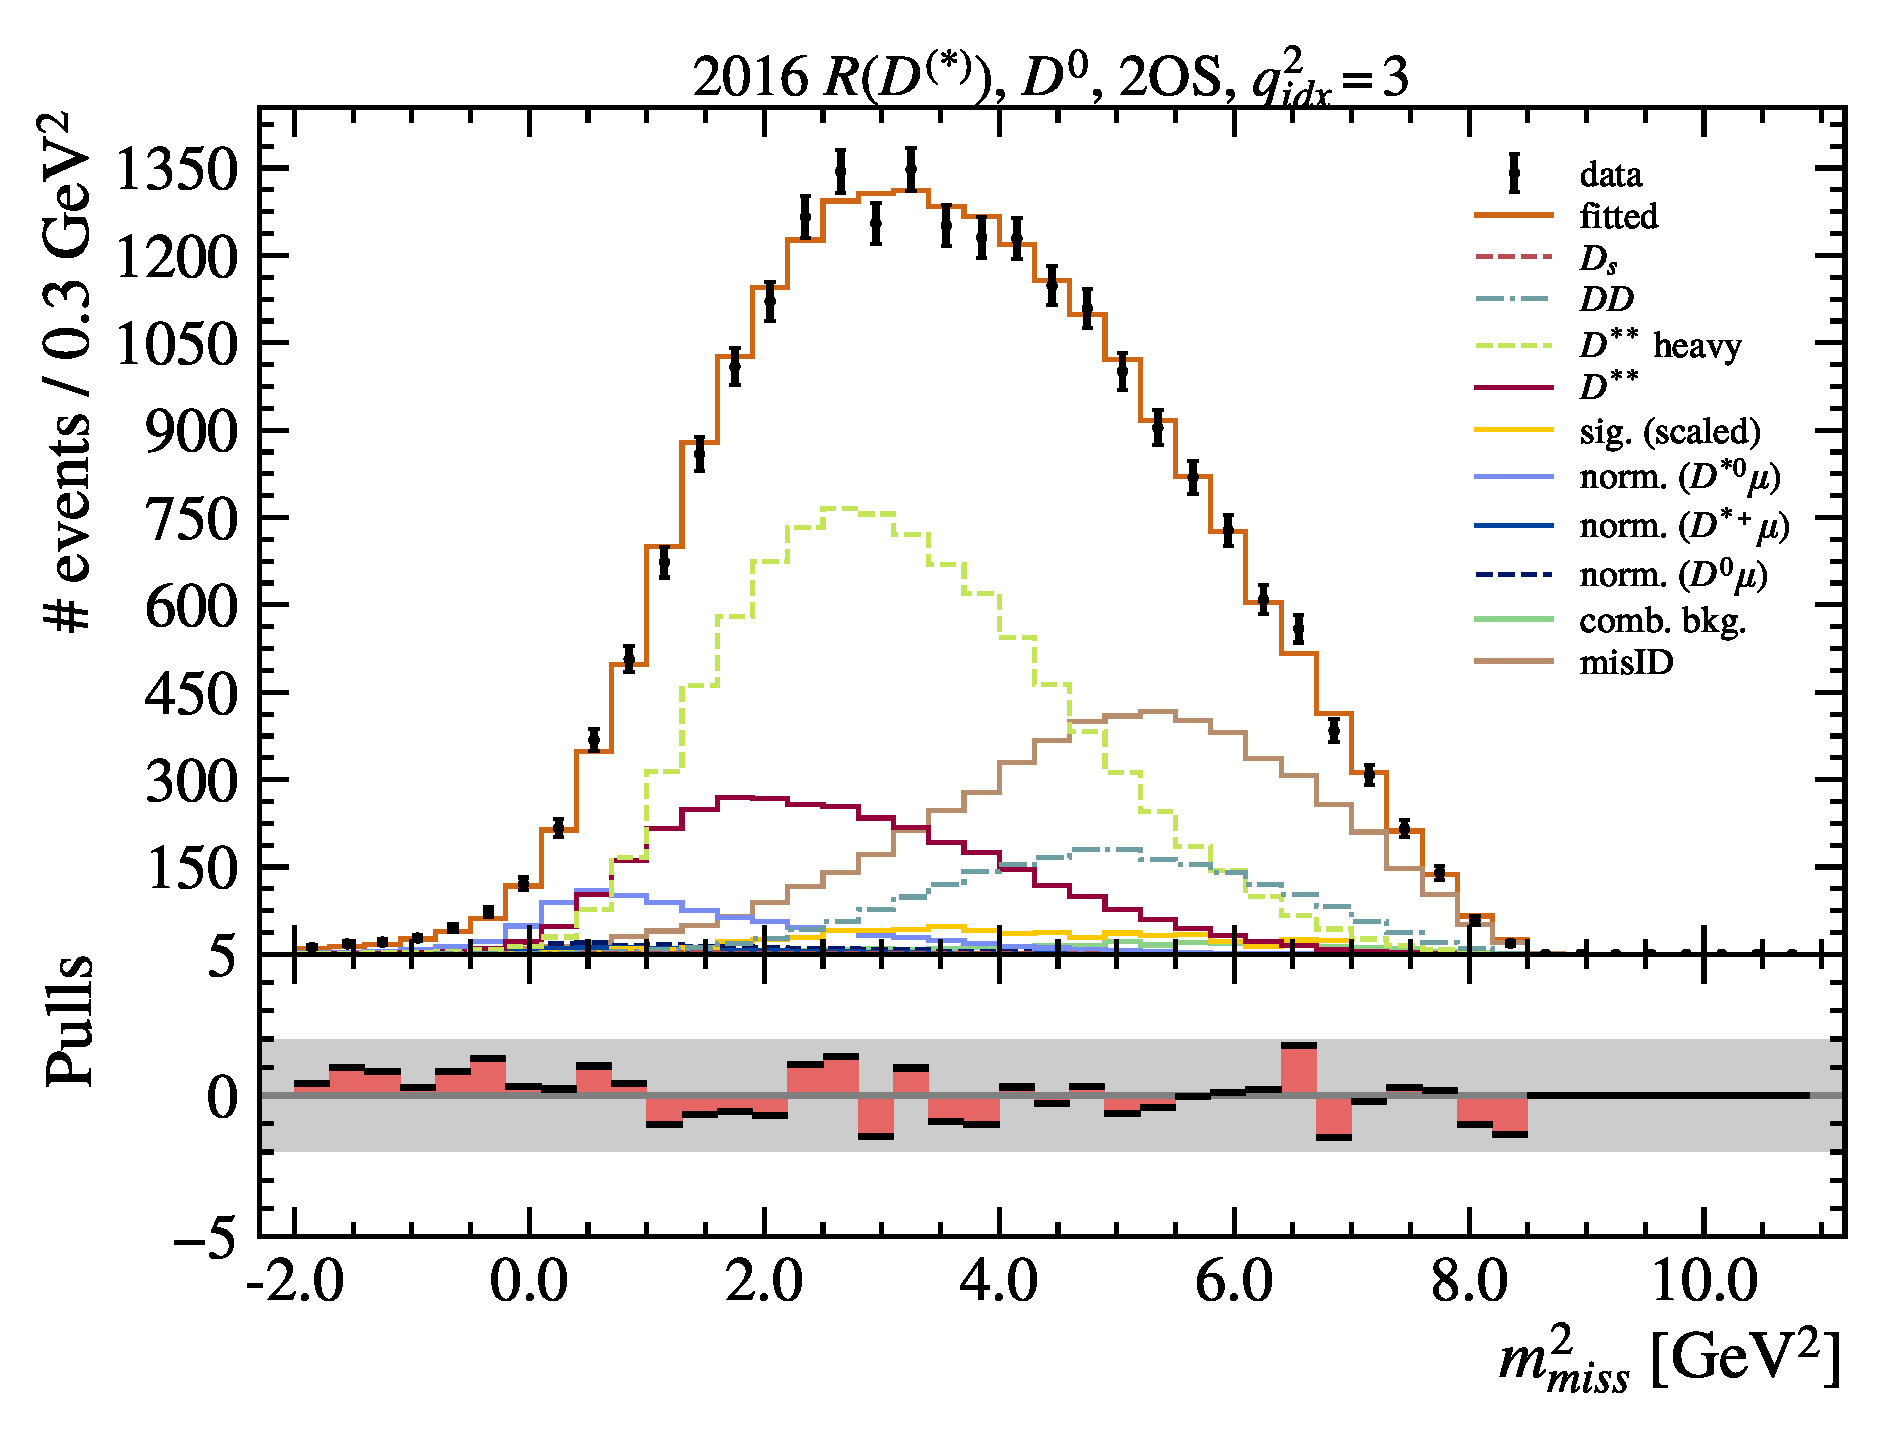
\includegraphics[width=0.24\textwidth]{./figs-fit-fit-results/ctrl-fit/lines_q2_slices/fit_result-lines_q2_idx3-D0-2os-mmiss2.pdf}
    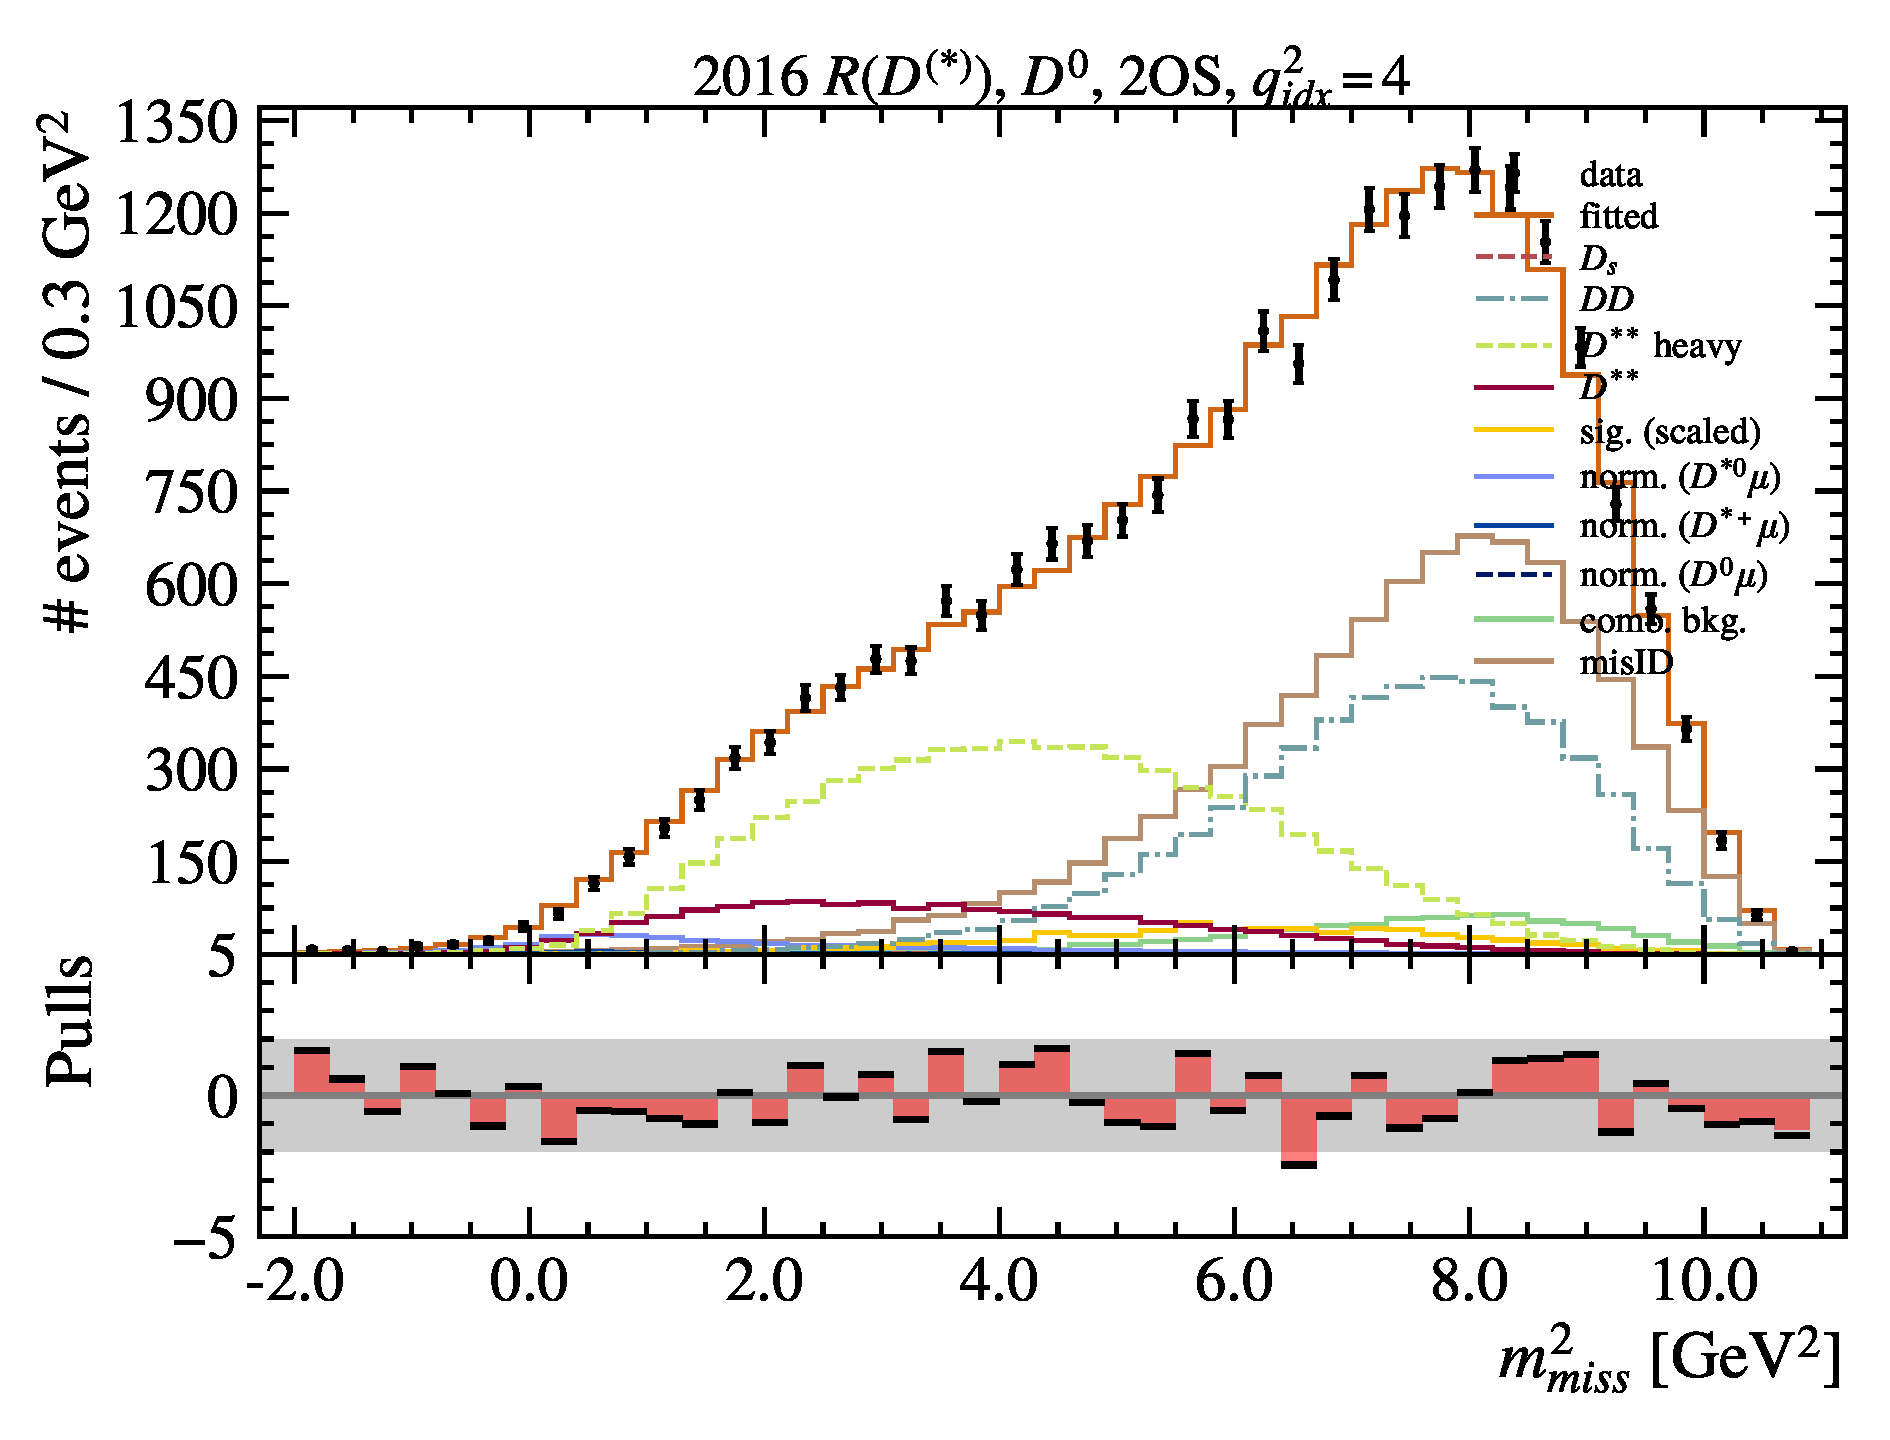
\includegraphics[width=0.24\textwidth]{./figs-fit-fit-results/ctrl-fit/lines_q2_slices/fit_result-lines_q2_idx4-D0-2os-mmiss2.pdf}

    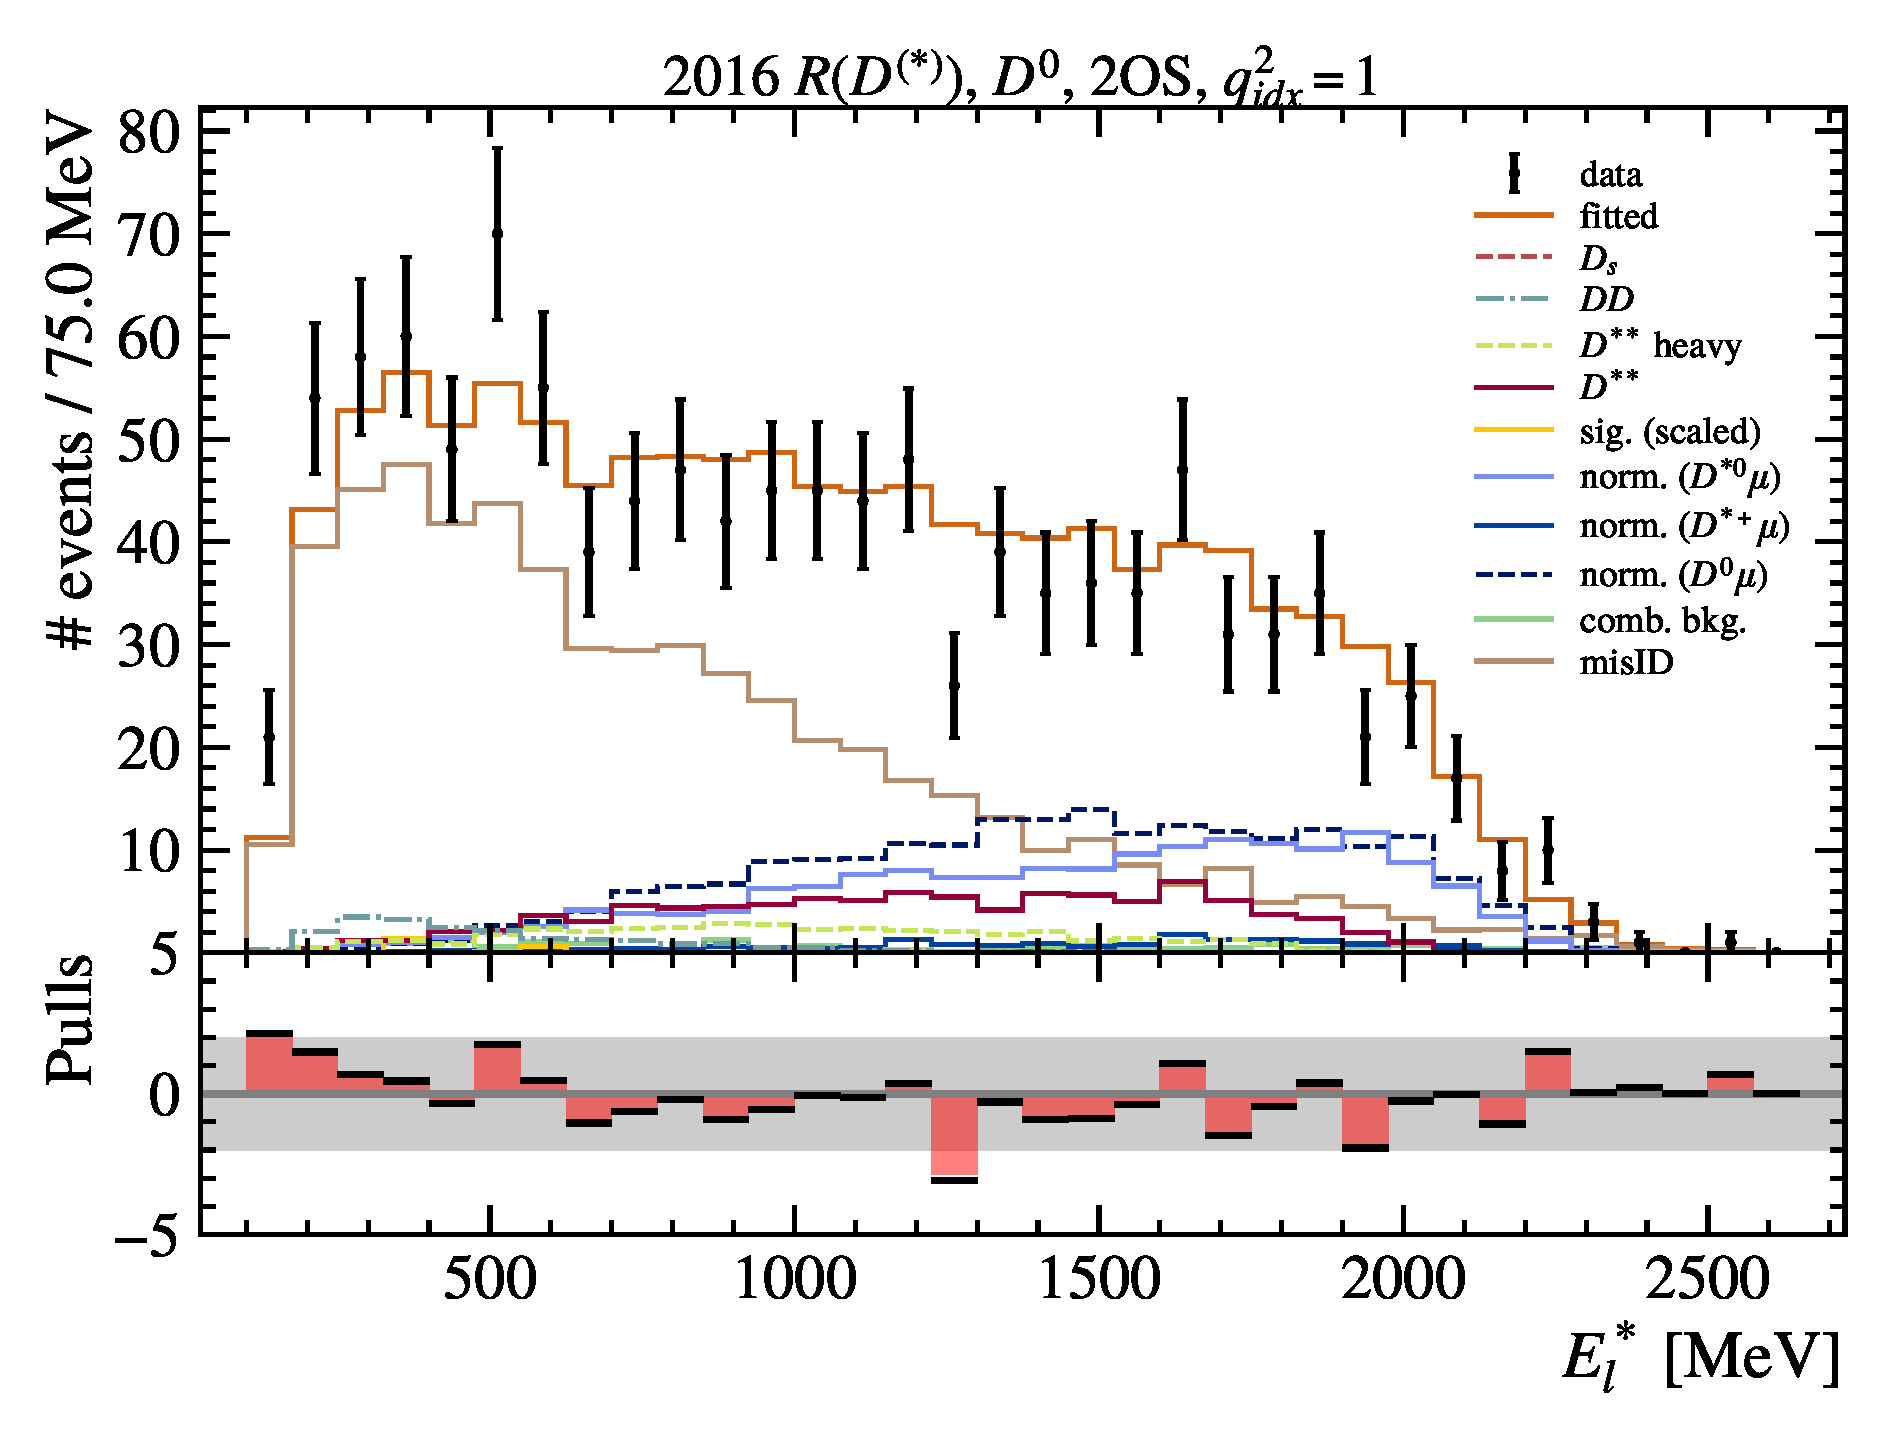
\includegraphics[width=0.24\textwidth]{./figs-fit-fit-results/ctrl-fit/lines_q2_slices/fit_result-lines_q2_idx1-D0-2os-el.pdf}
    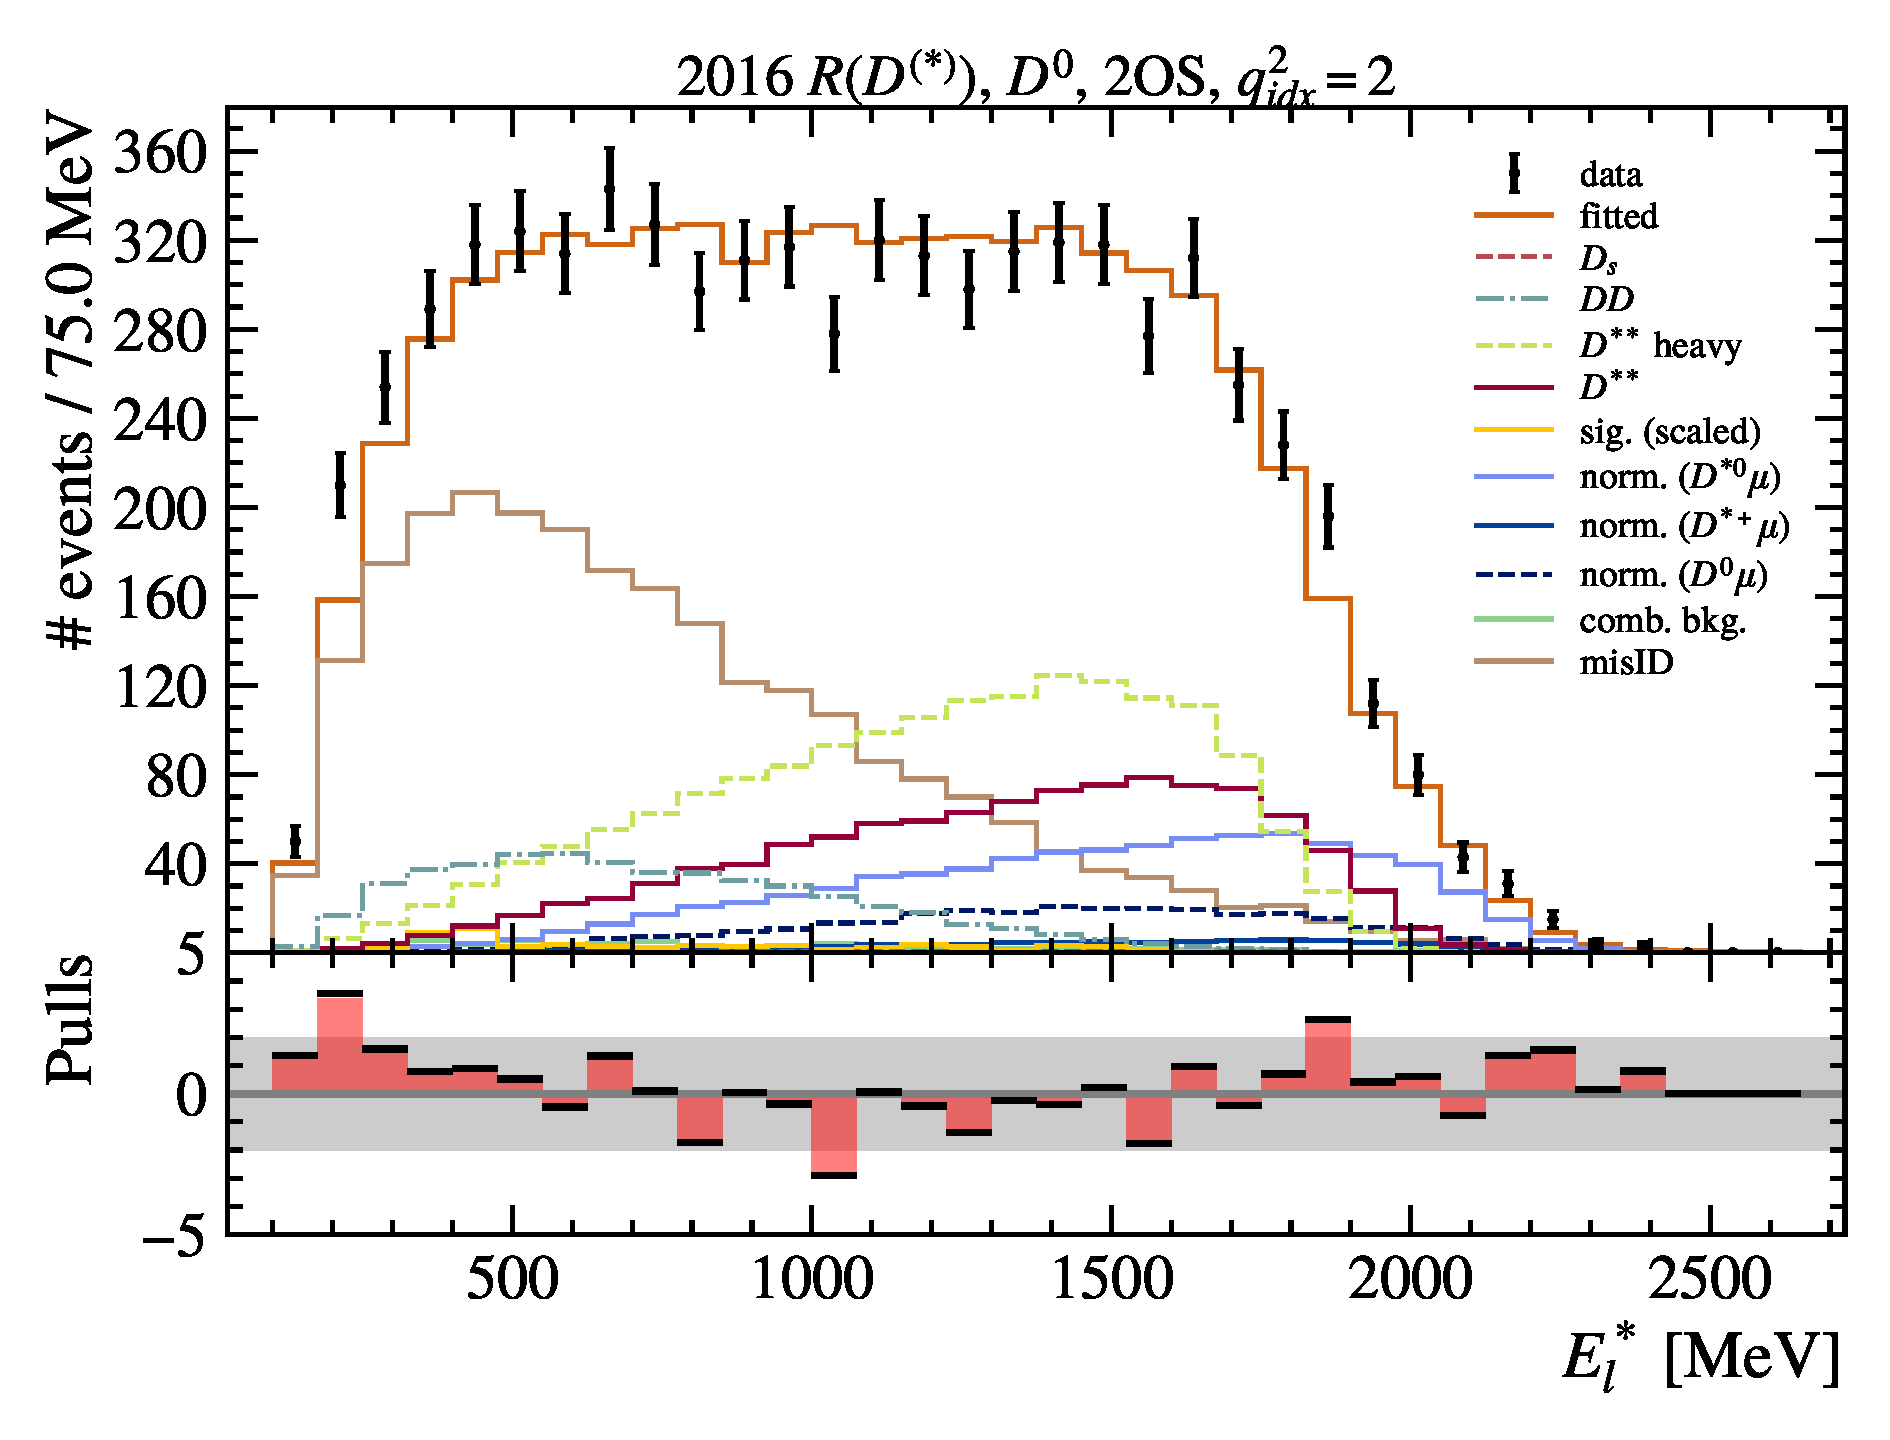
\includegraphics[width=0.24\textwidth]{./figs-fit-fit-results/ctrl-fit/lines_q2_slices/fit_result-lines_q2_idx2-D0-2os-el.pdf}
    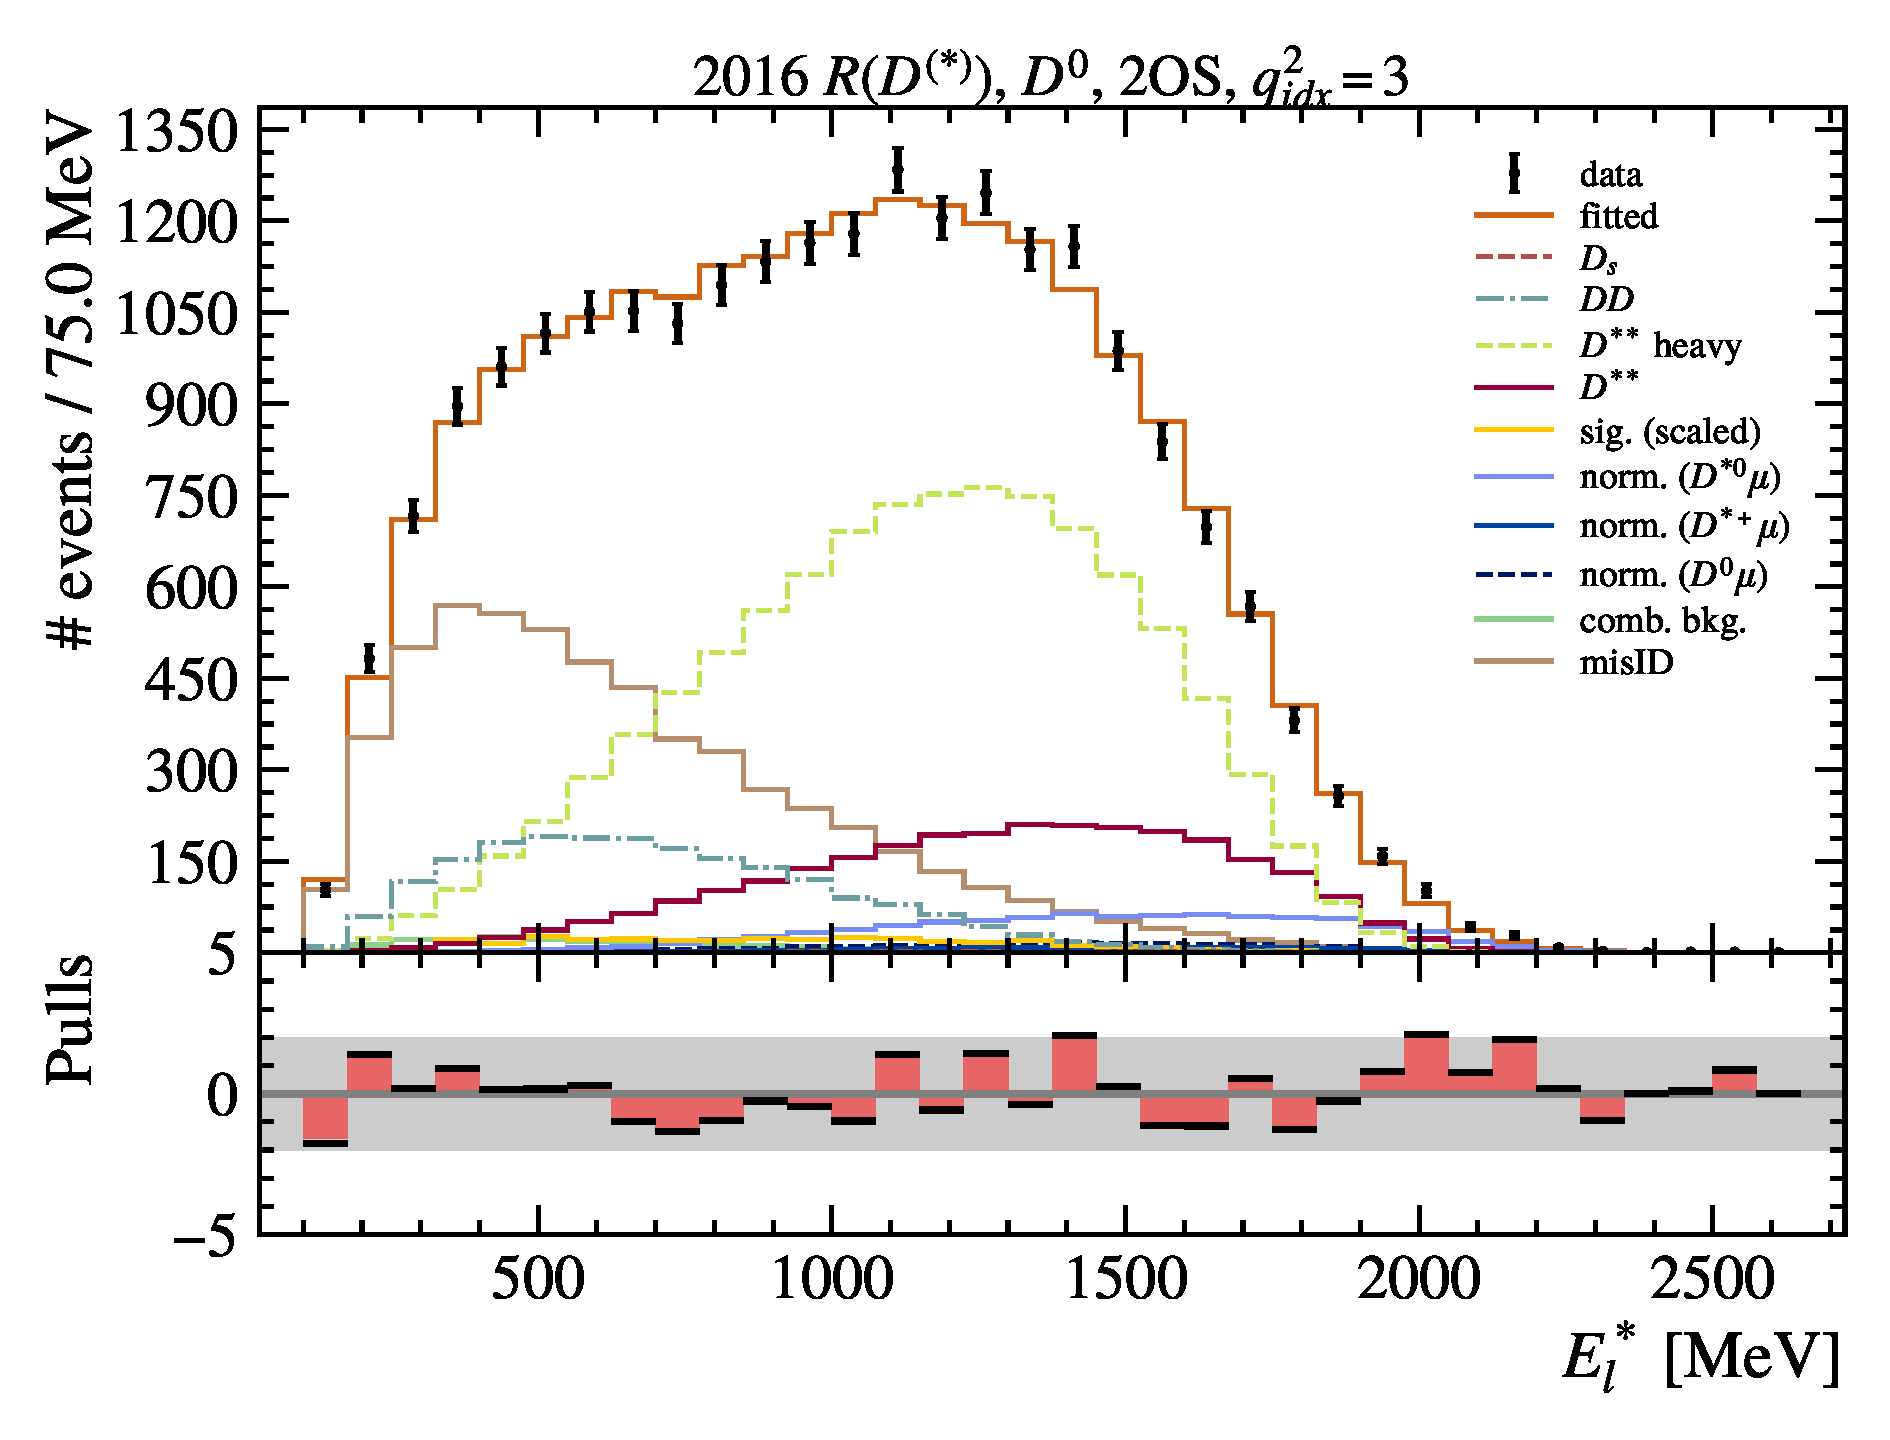
\includegraphics[width=0.24\textwidth]{./figs-fit-fit-results/ctrl-fit/lines_q2_slices/fit_result-lines_q2_idx3-D0-2os-el.pdf}
    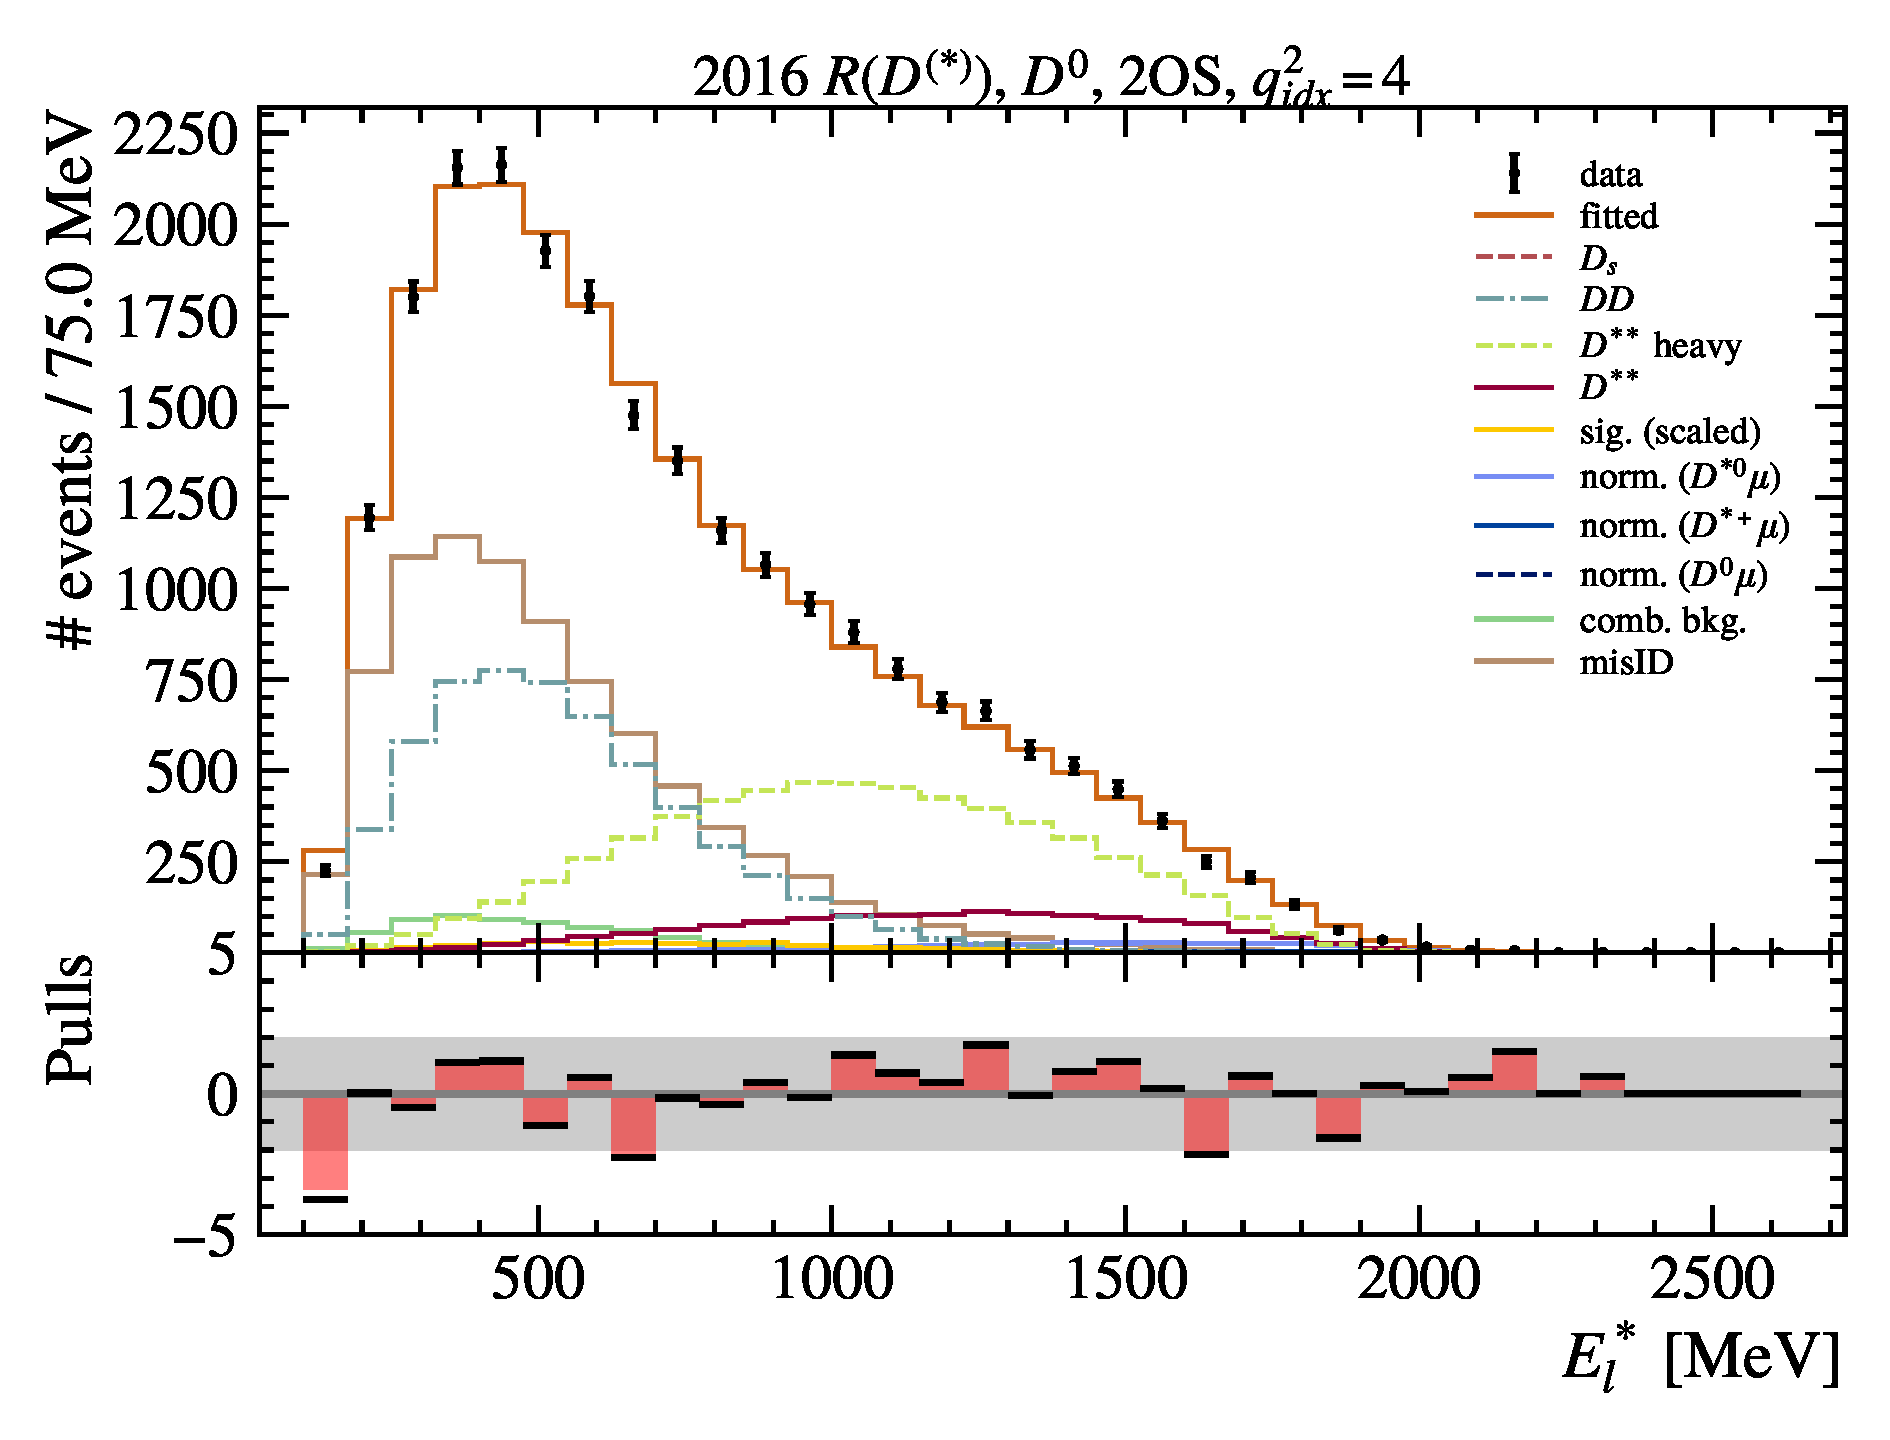
\includegraphics[width=0.24\textwidth]{./figs-fit-fit-results/ctrl-fit/lines_q2_slices/fit_result-lines_q2_idx4-D0-2os-el.pdf}

    \caption{Control fit for 2OS sample, \Dz channel.}
    \label{fig:ctrl-2os-d0}
\end{figure}

\begin{figure}[!htb]
    \centering
    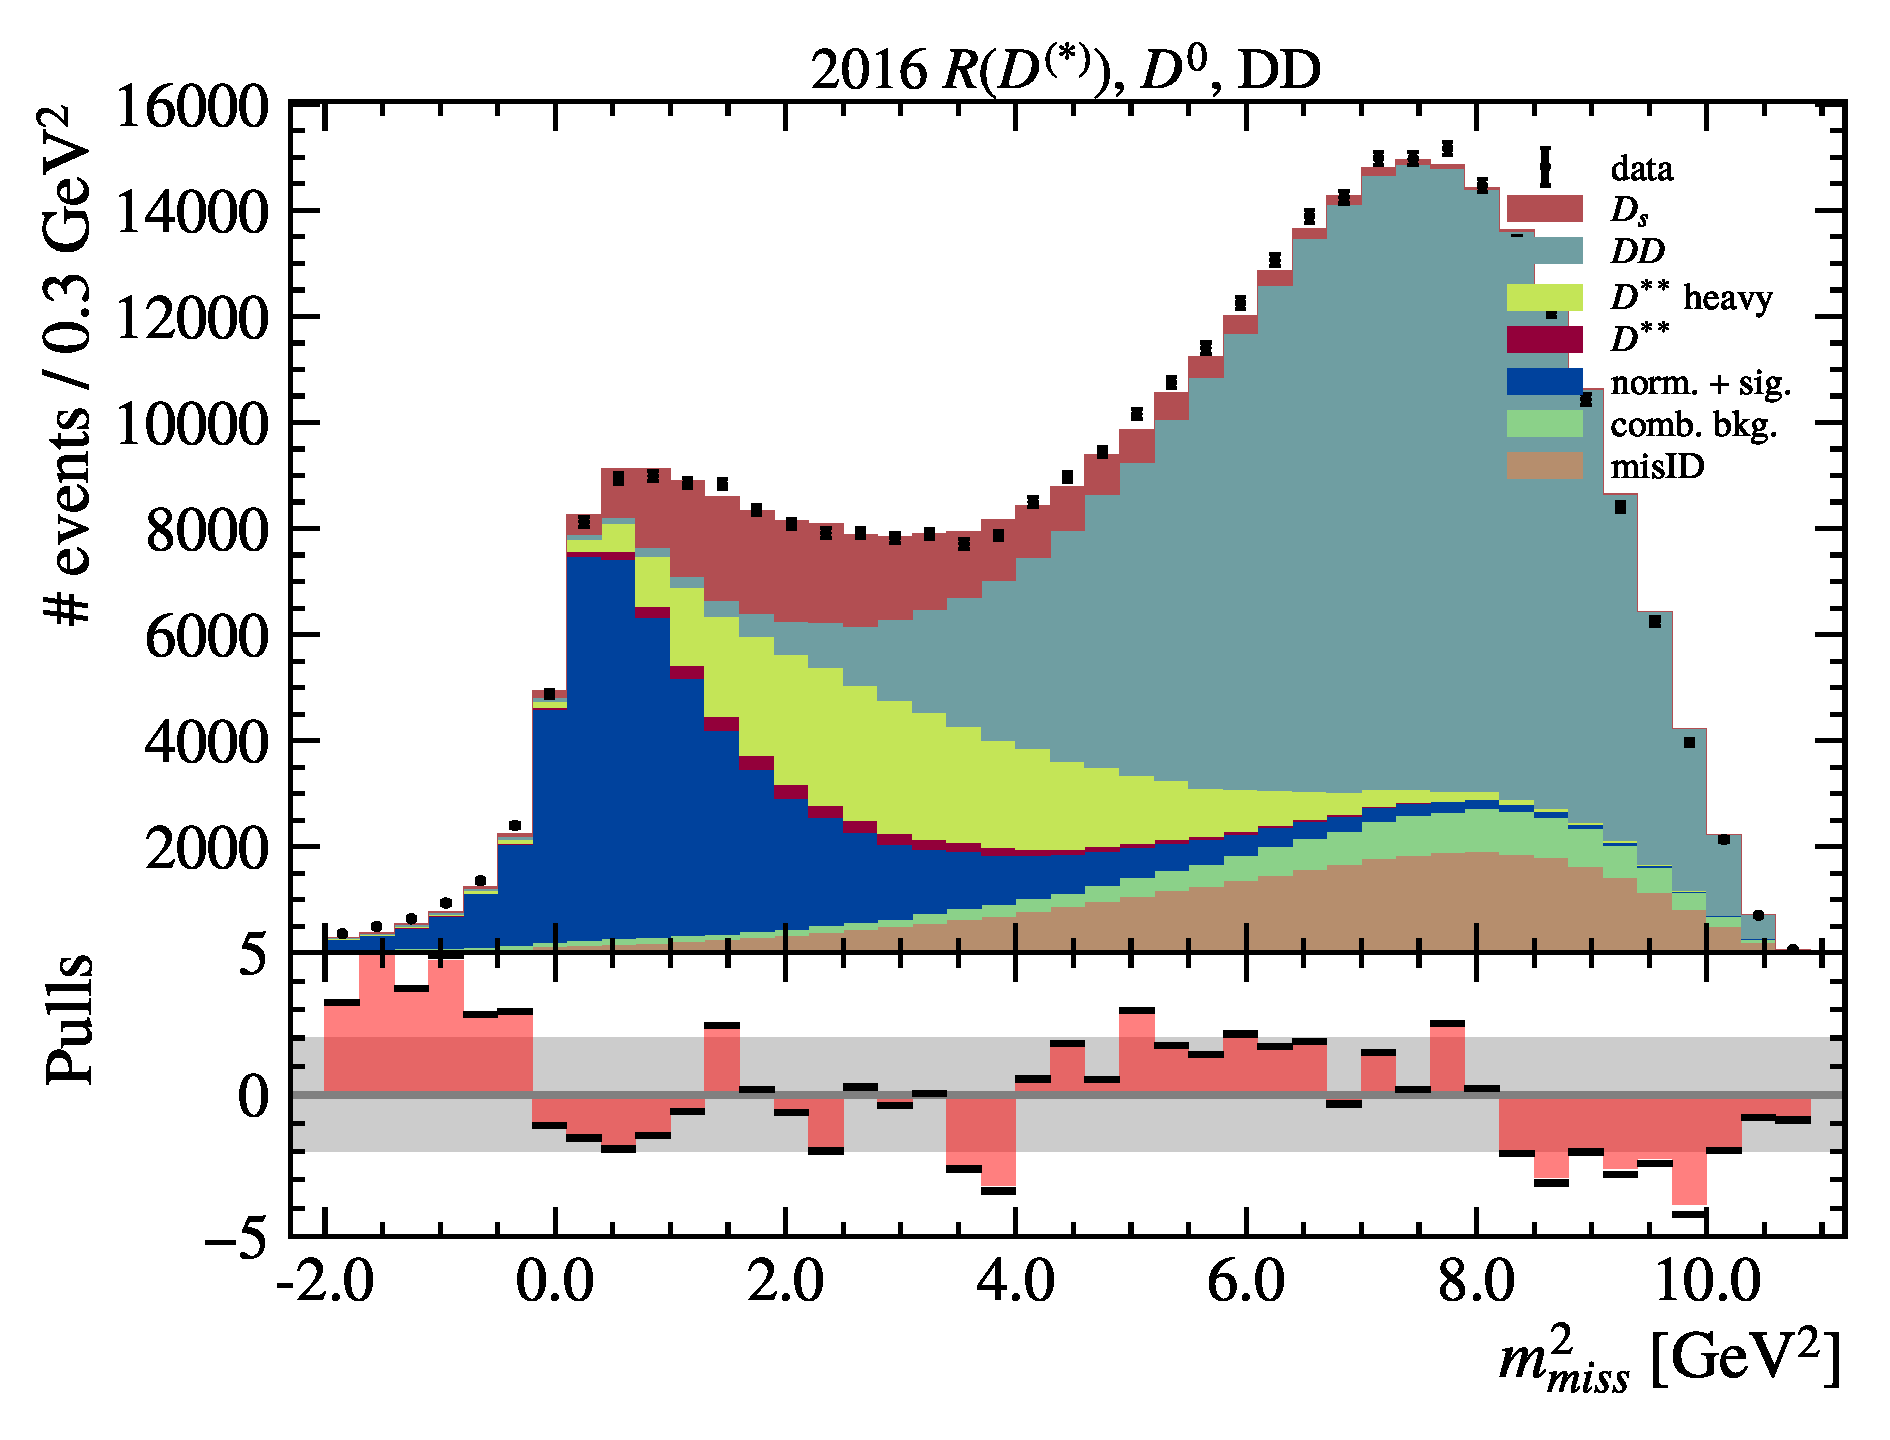
\includegraphics[width=0.32\textwidth]{./figs-fit-fit-results/ctrl-fit/stacked/fit_result-stacked-D0-dd-mmiss2.pdf}
    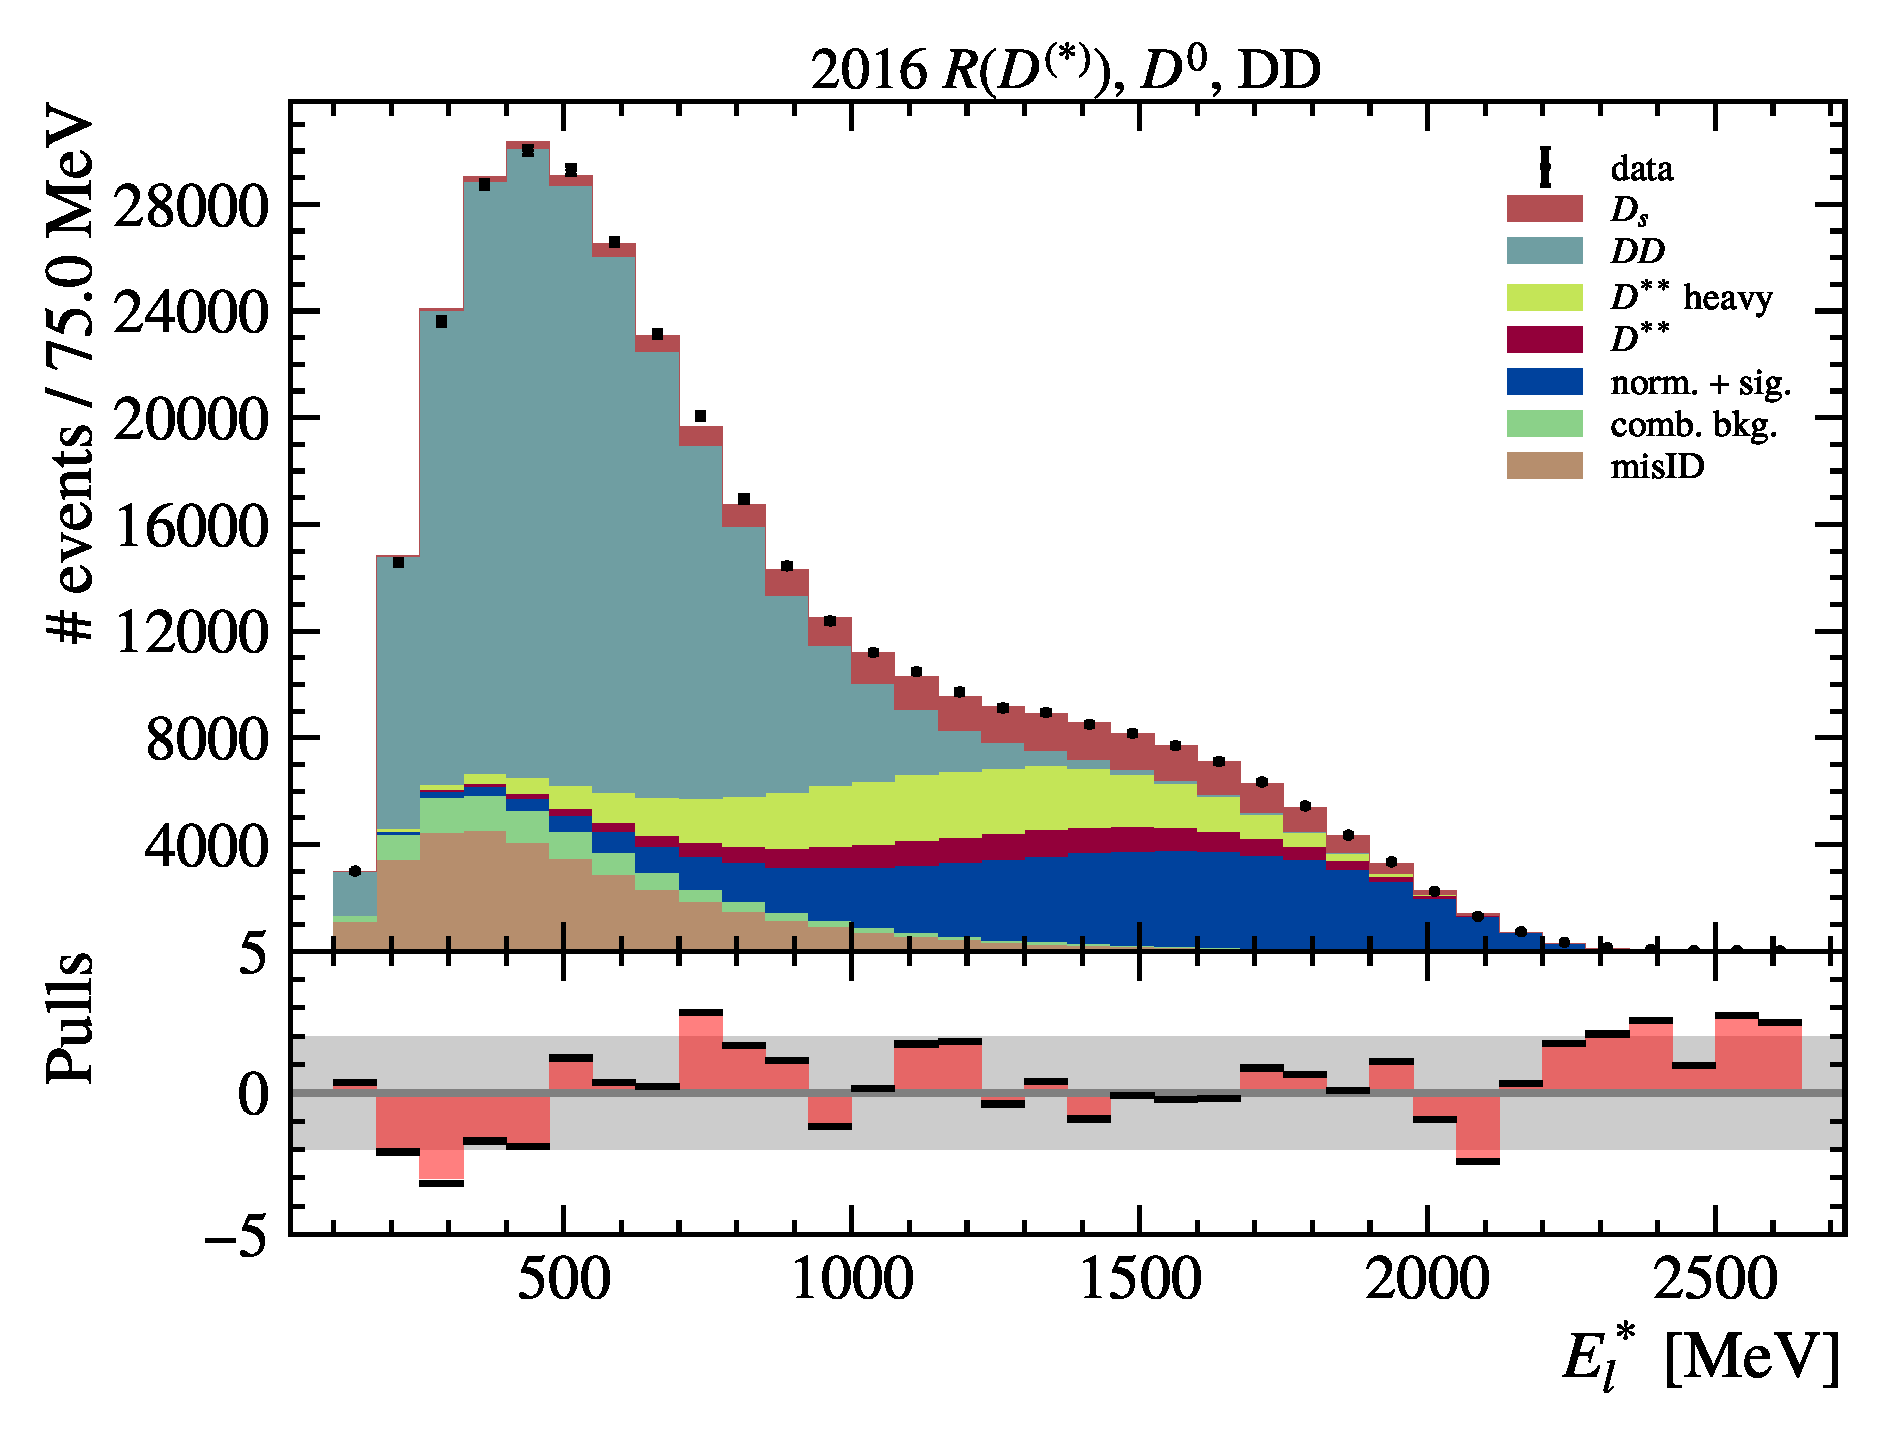
\includegraphics[width=0.32\textwidth]{./figs-fit-fit-results/ctrl-fit/stacked/fit_result-stacked-D0-dd-el.pdf}
    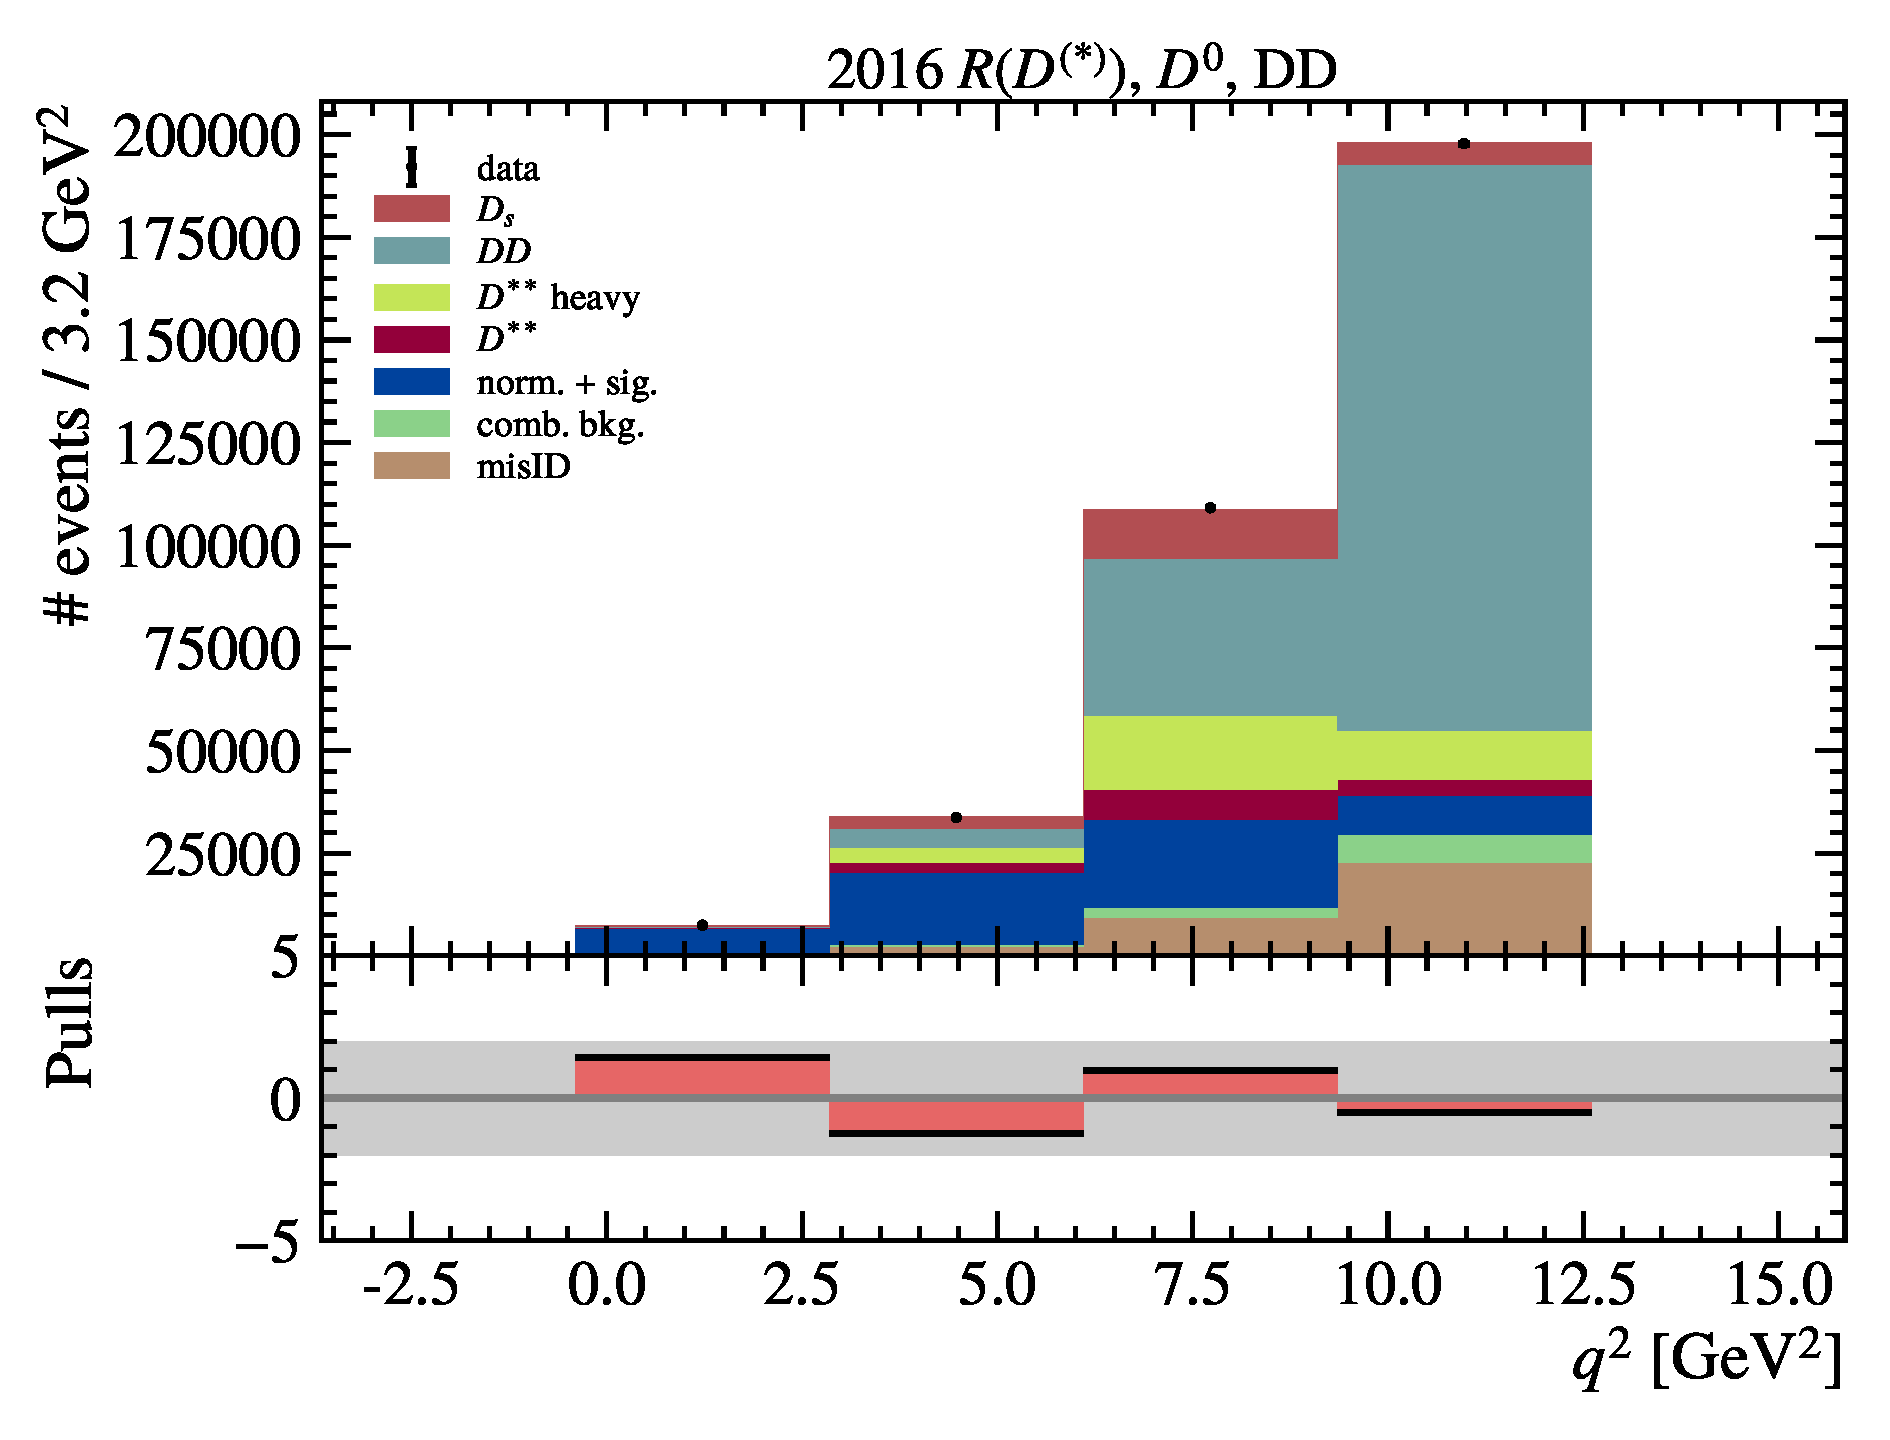
\includegraphics[width=0.32\textwidth]{./figs-fit-fit-results/ctrl-fit/stacked/fit_result-stacked-D0-dd-q2.pdf}

    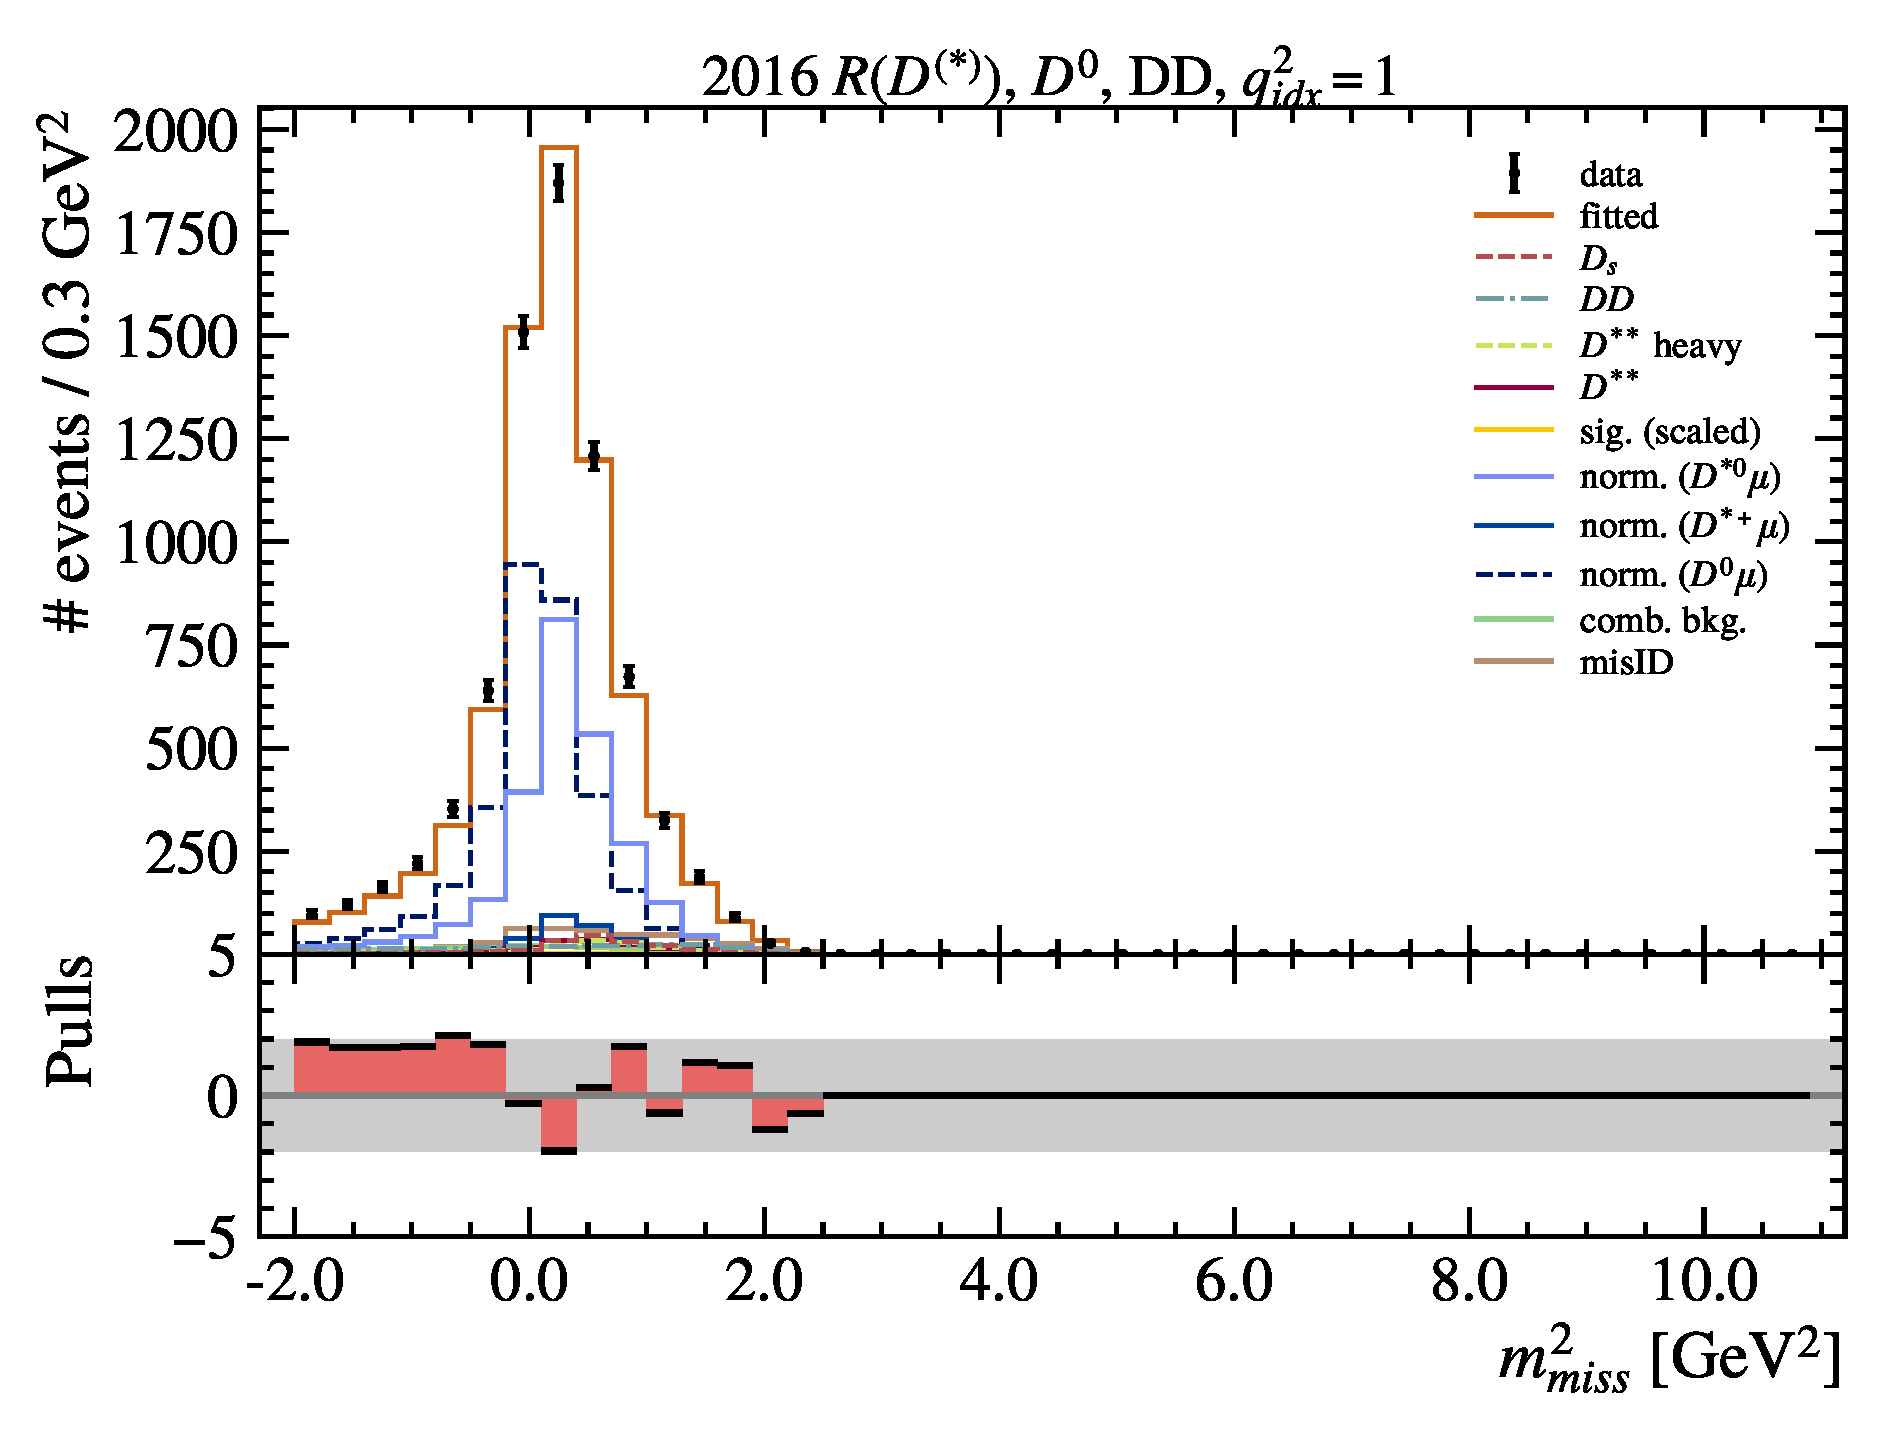
\includegraphics[width=0.24\textwidth]{./figs-fit-fit-results/ctrl-fit/lines_q2_slices/fit_result-lines_q2_idx1-D0-dd-mmiss2.pdf}
    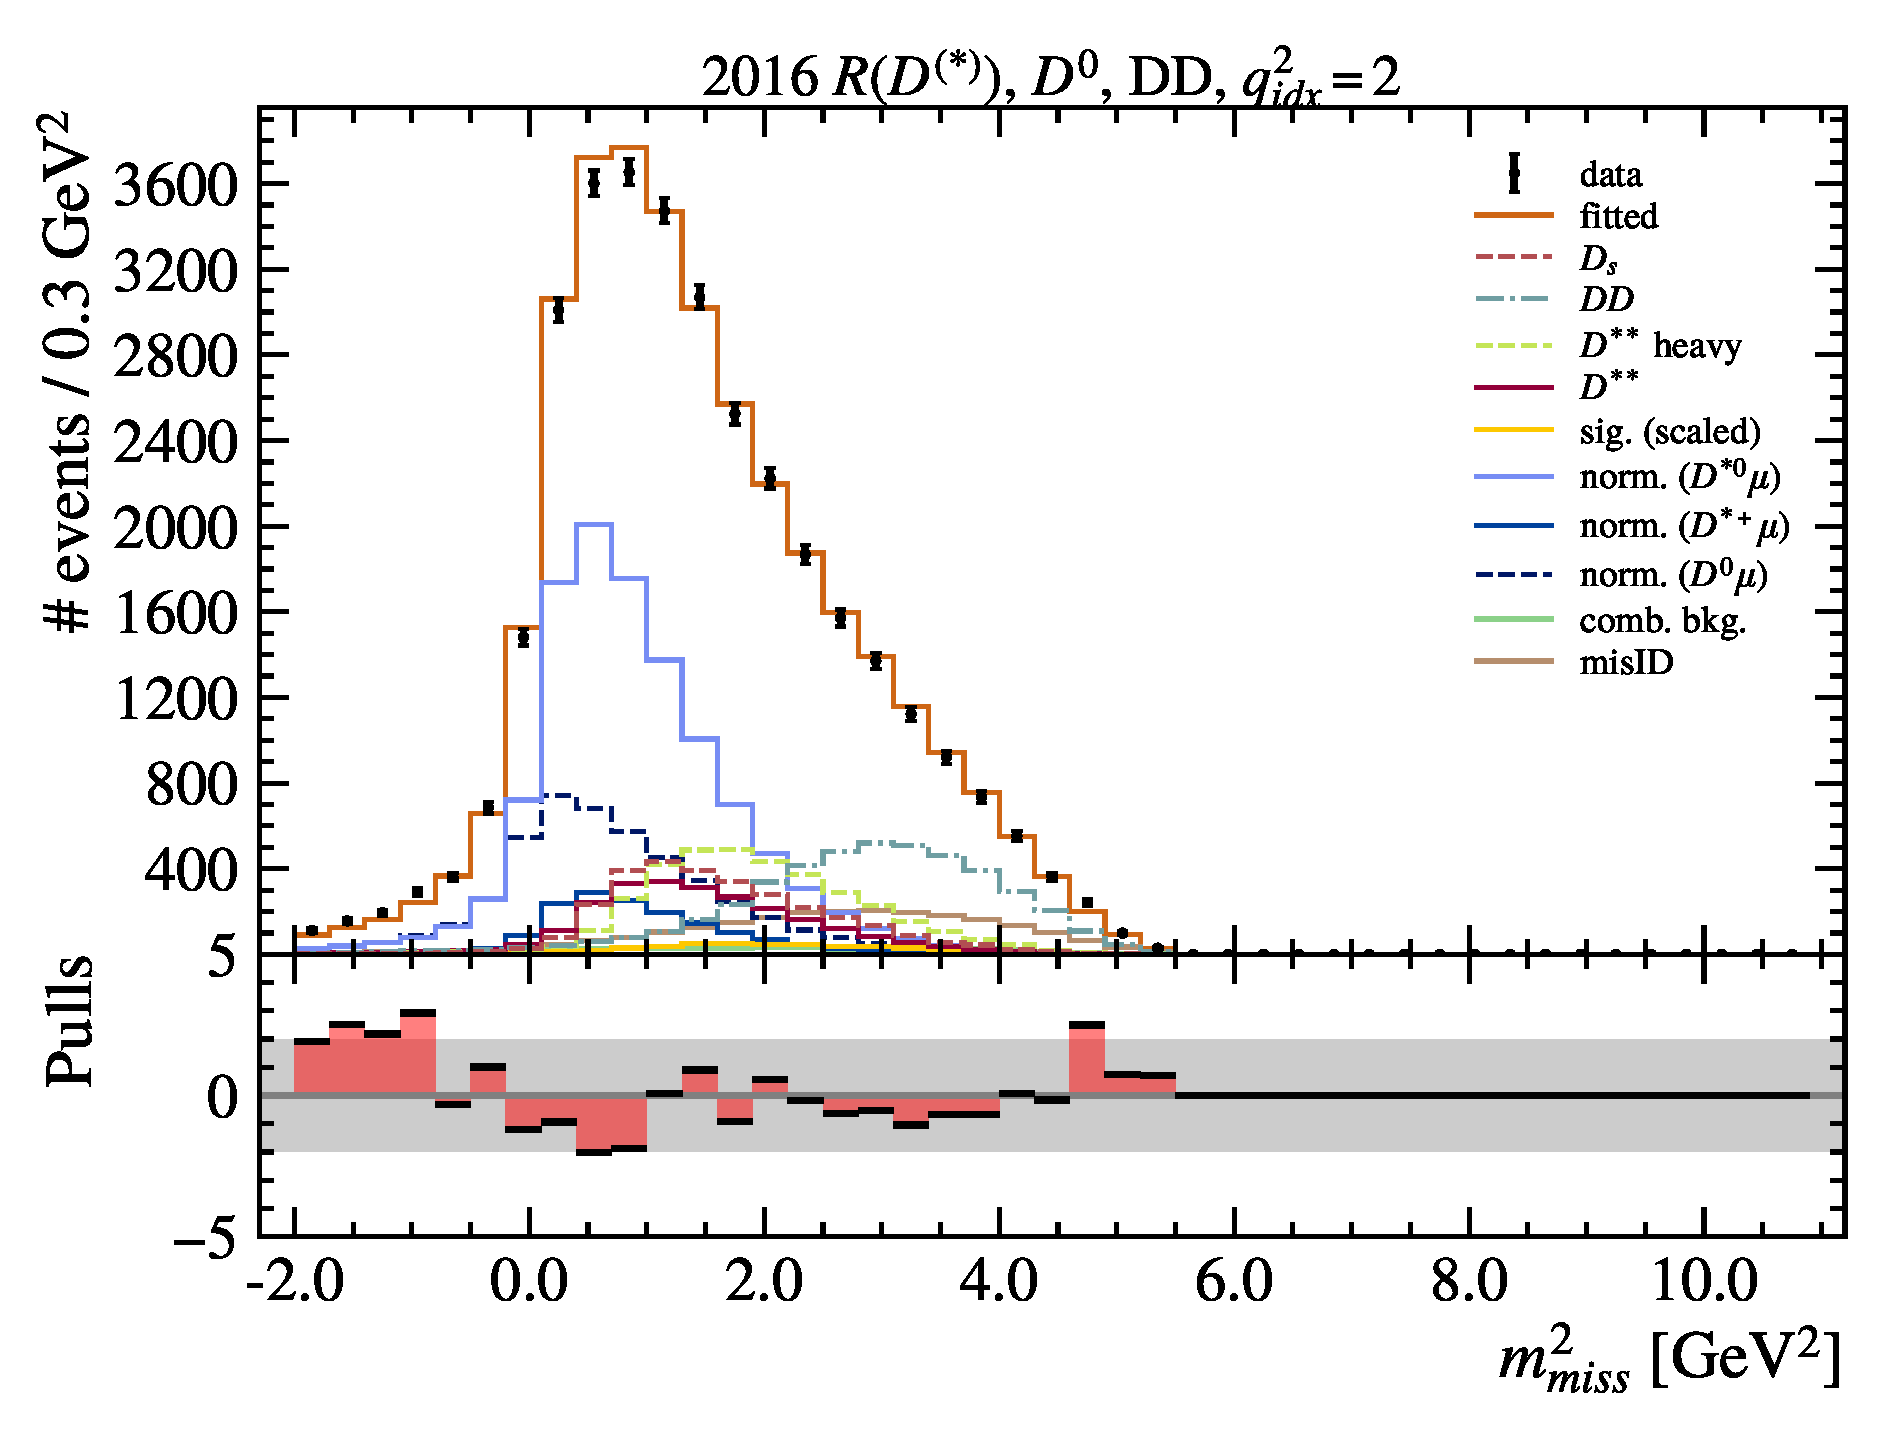
\includegraphics[width=0.24\textwidth]{./figs-fit-fit-results/ctrl-fit/lines_q2_slices/fit_result-lines_q2_idx2-D0-dd-mmiss2.pdf}
    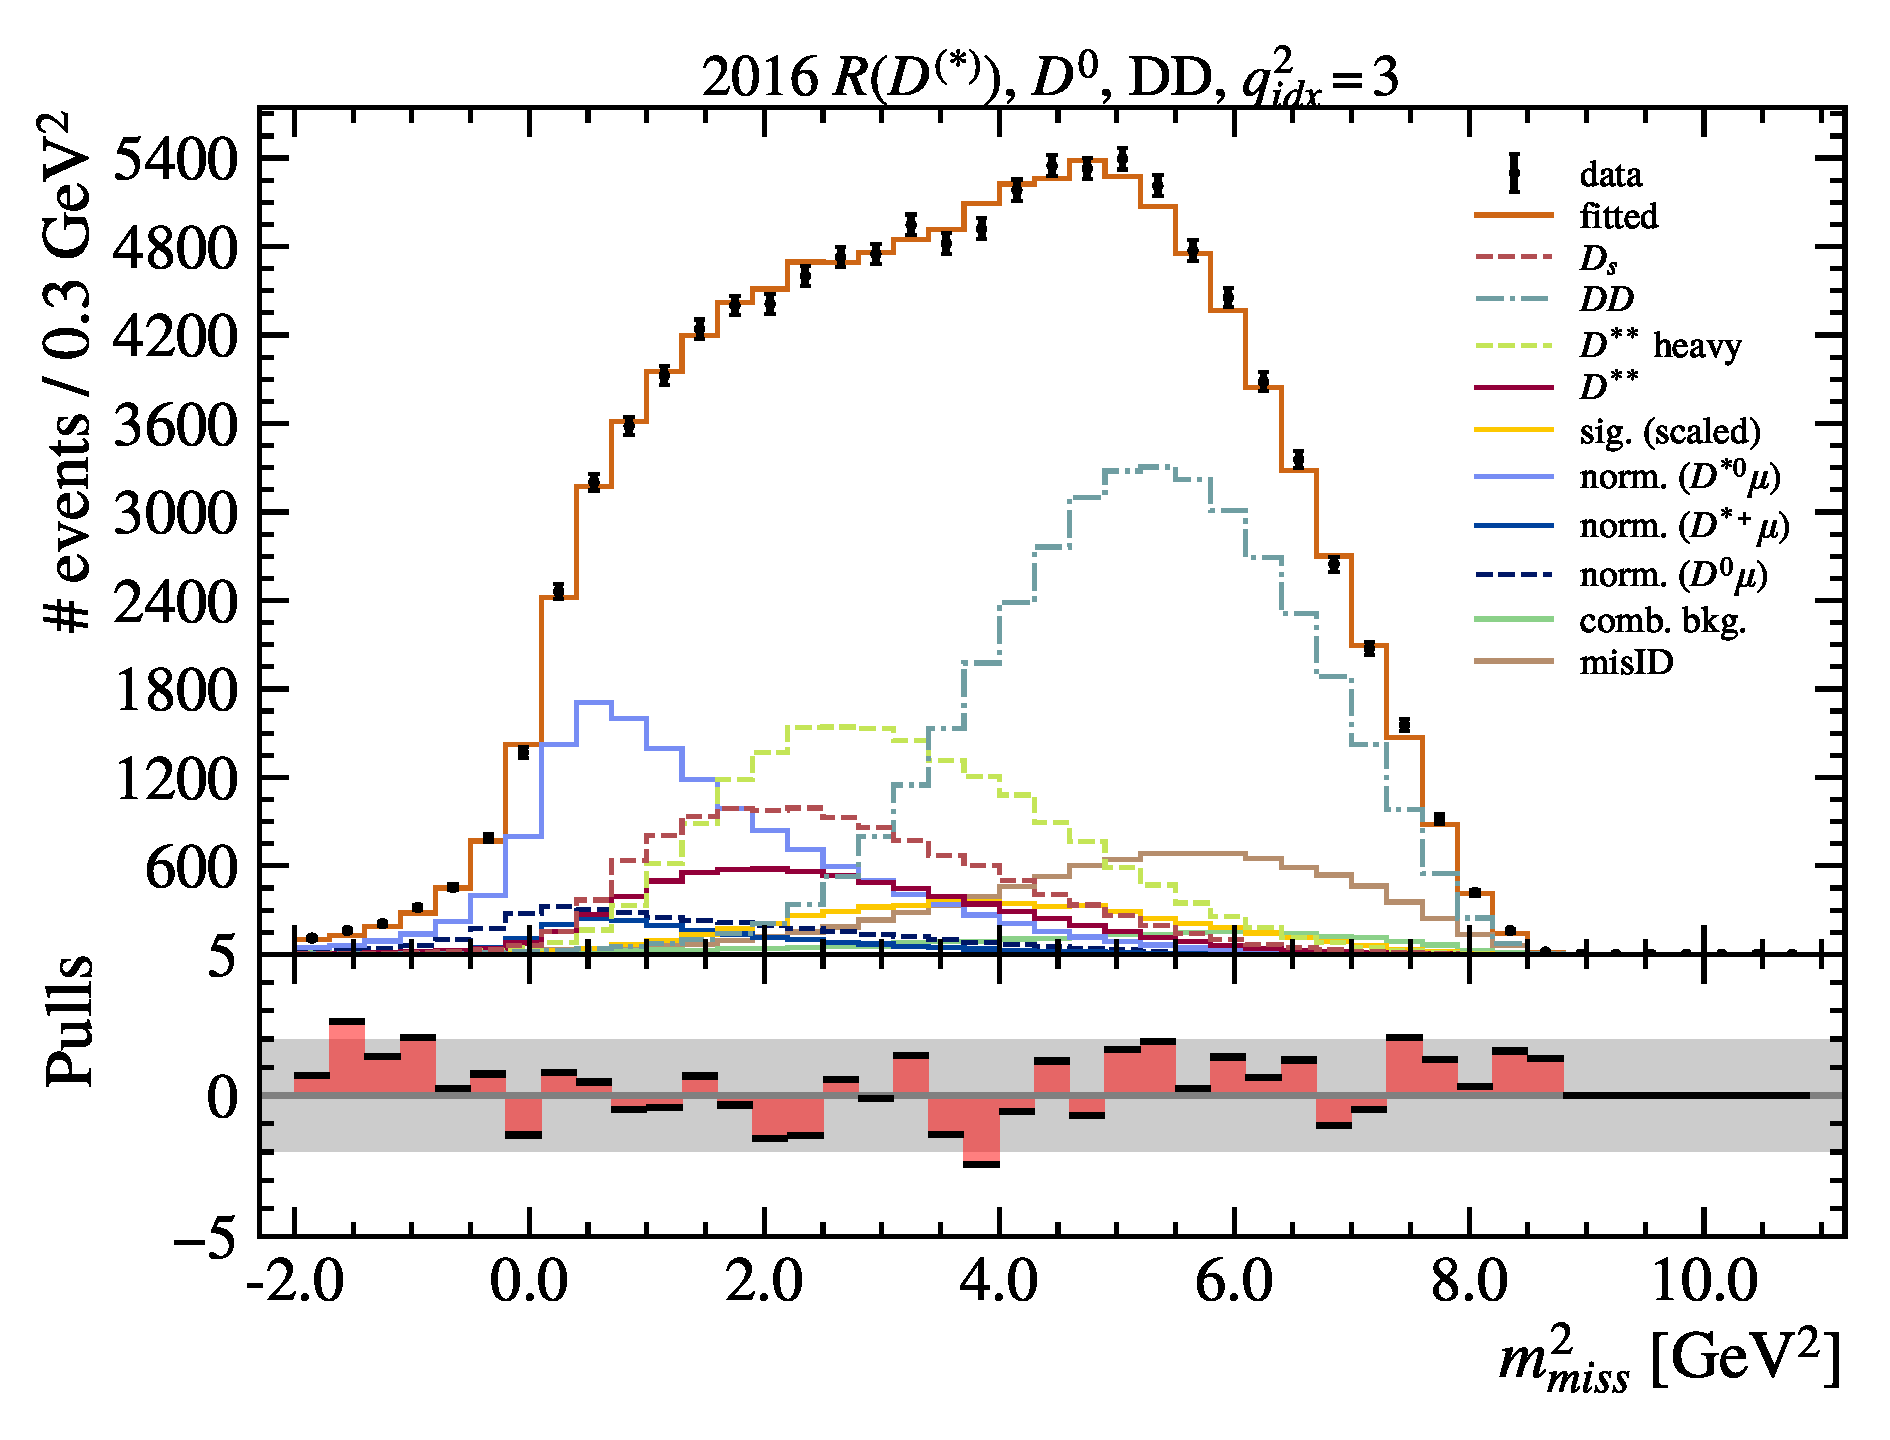
\includegraphics[width=0.24\textwidth]{./figs-fit-fit-results/ctrl-fit/lines_q2_slices/fit_result-lines_q2_idx3-D0-dd-mmiss2.pdf}
    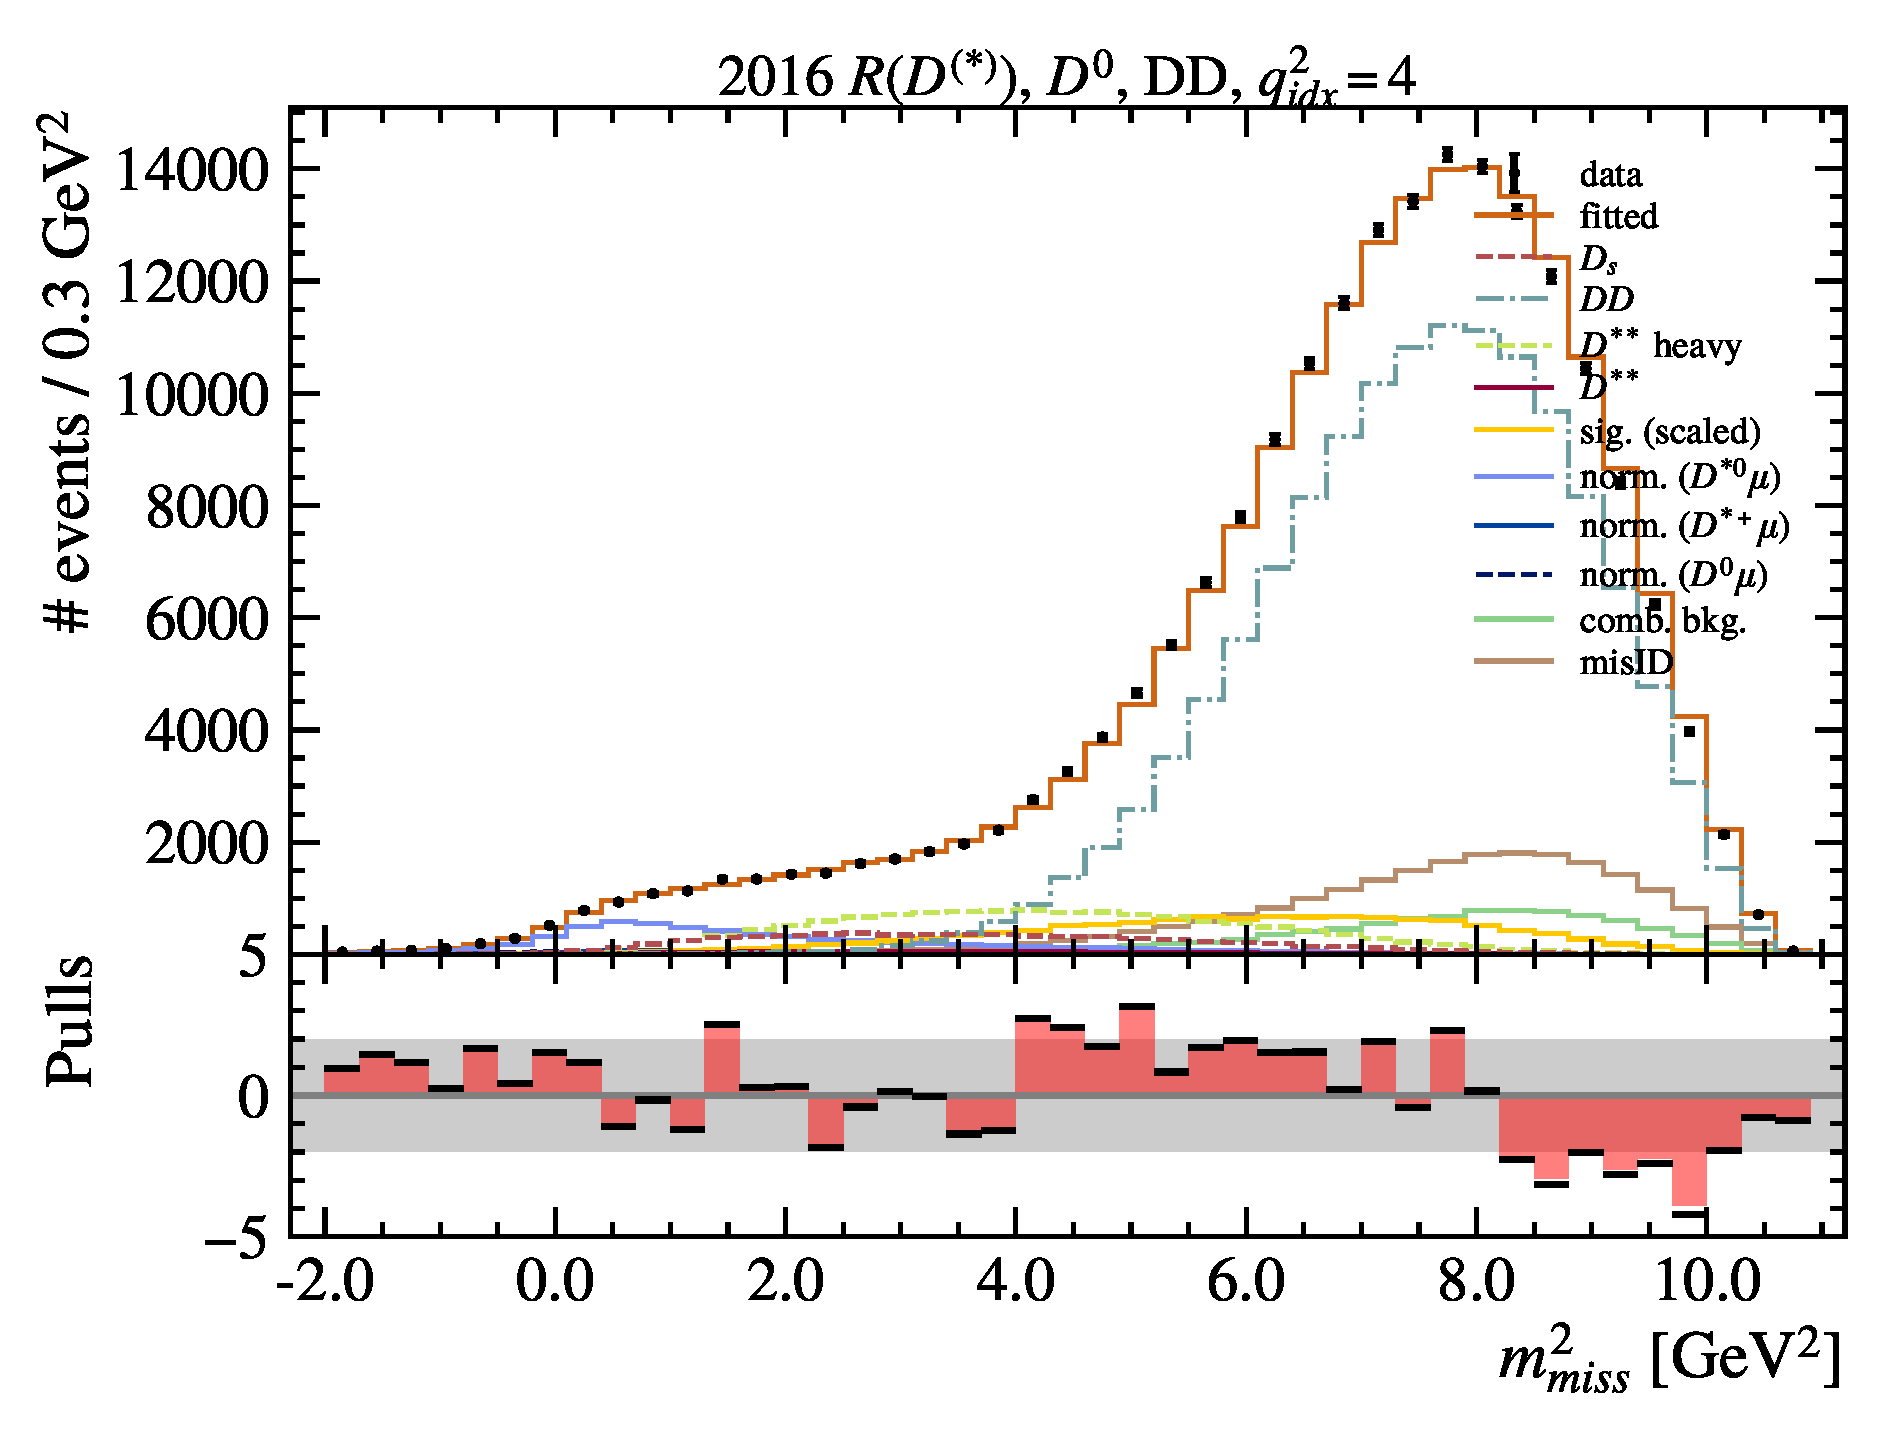
\includegraphics[width=0.24\textwidth]{./figs-fit-fit-results/ctrl-fit/lines_q2_slices/fit_result-lines_q2_idx4-D0-dd-mmiss2.pdf}

    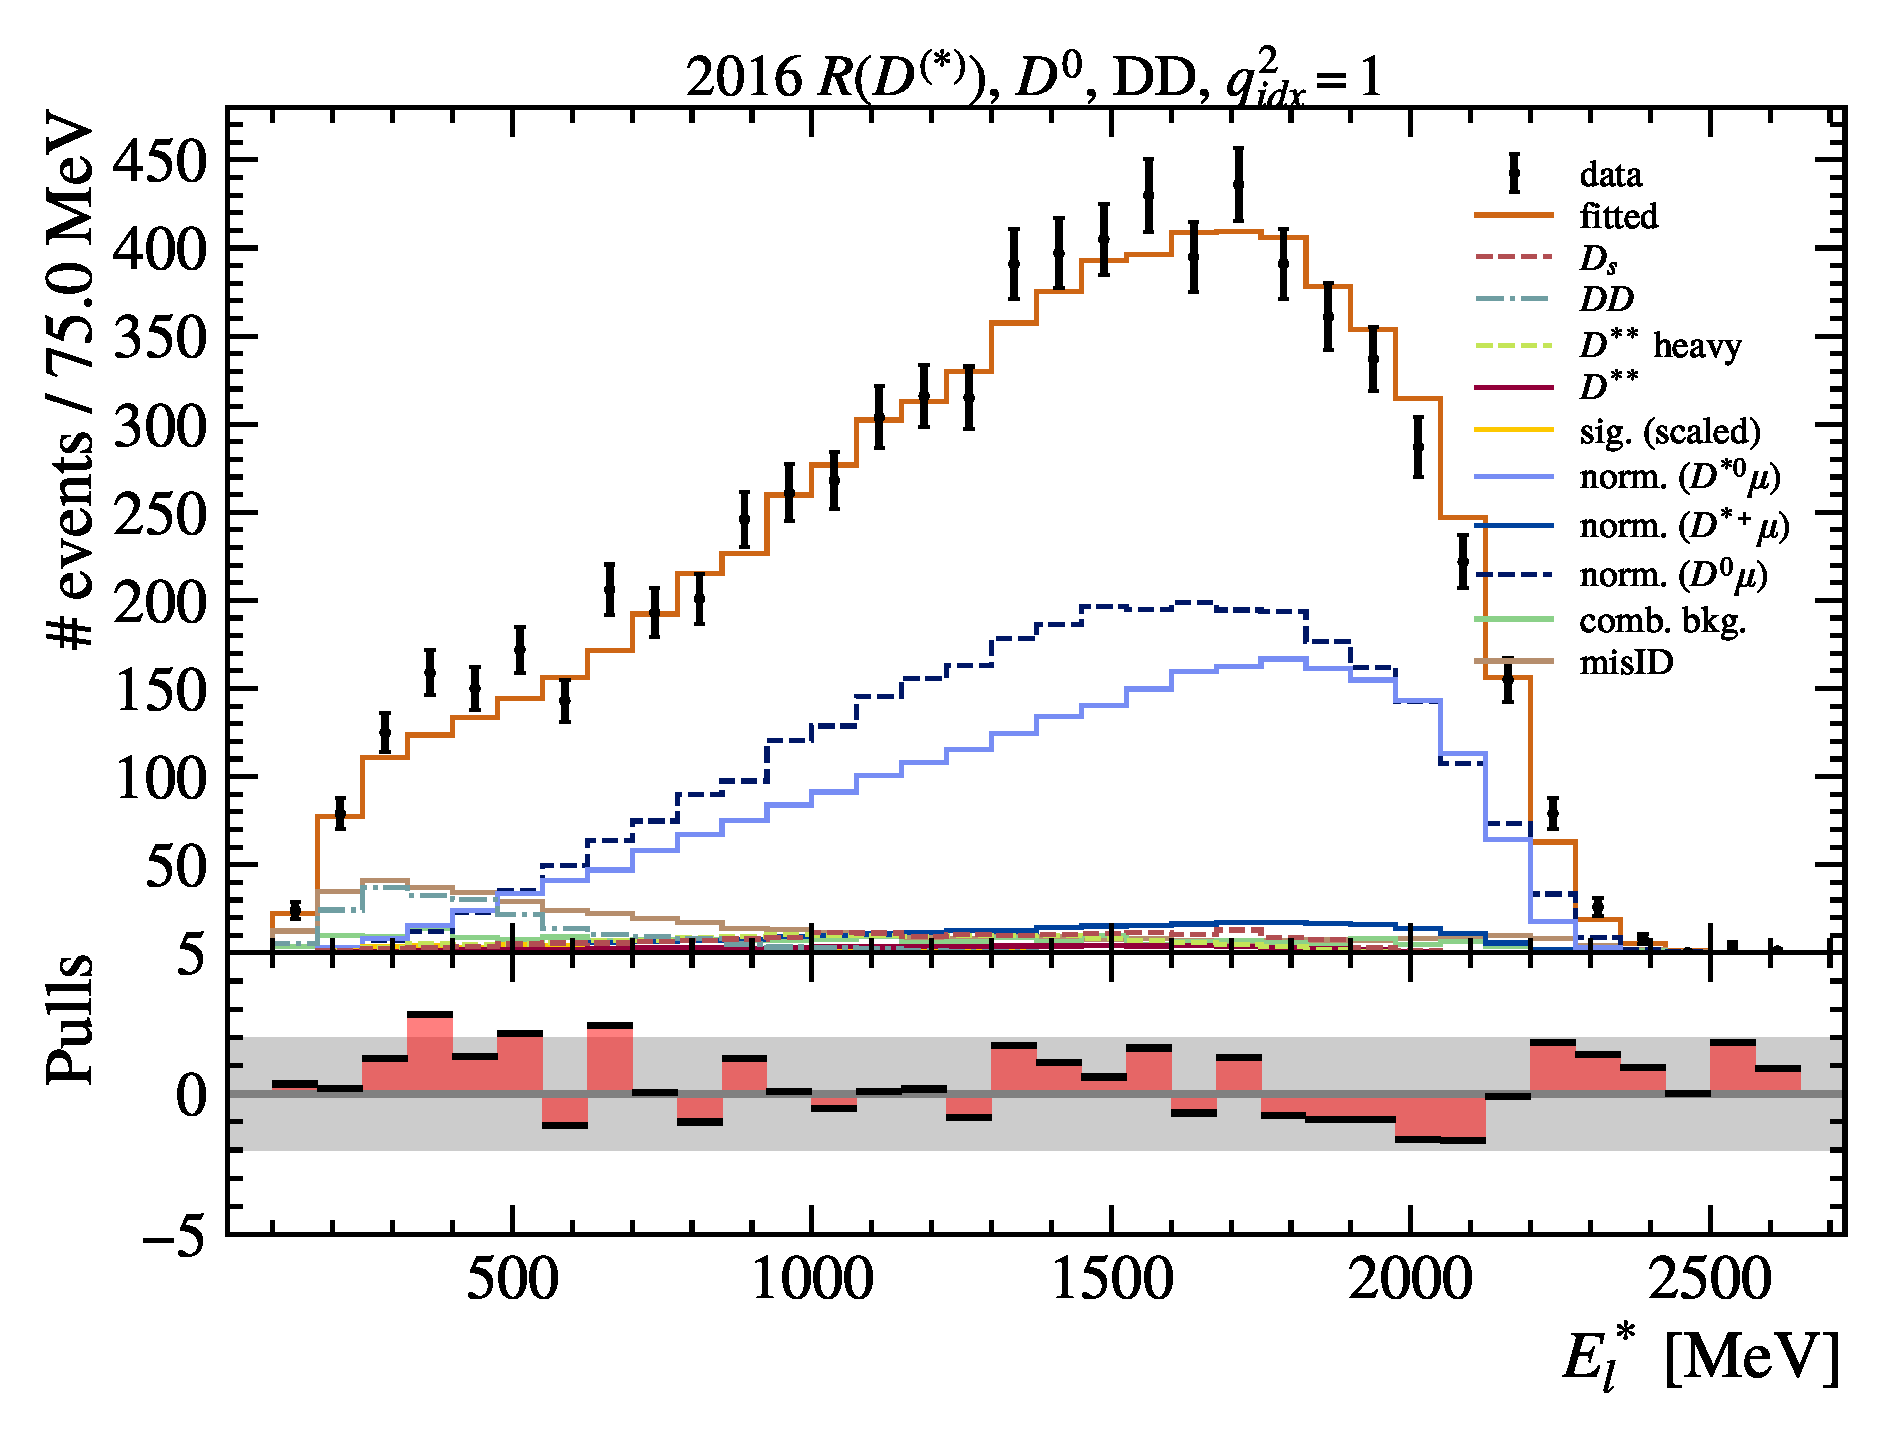
\includegraphics[width=0.24\textwidth]{./figs-fit-fit-results/ctrl-fit/lines_q2_slices/fit_result-lines_q2_idx1-D0-dd-el.pdf}
    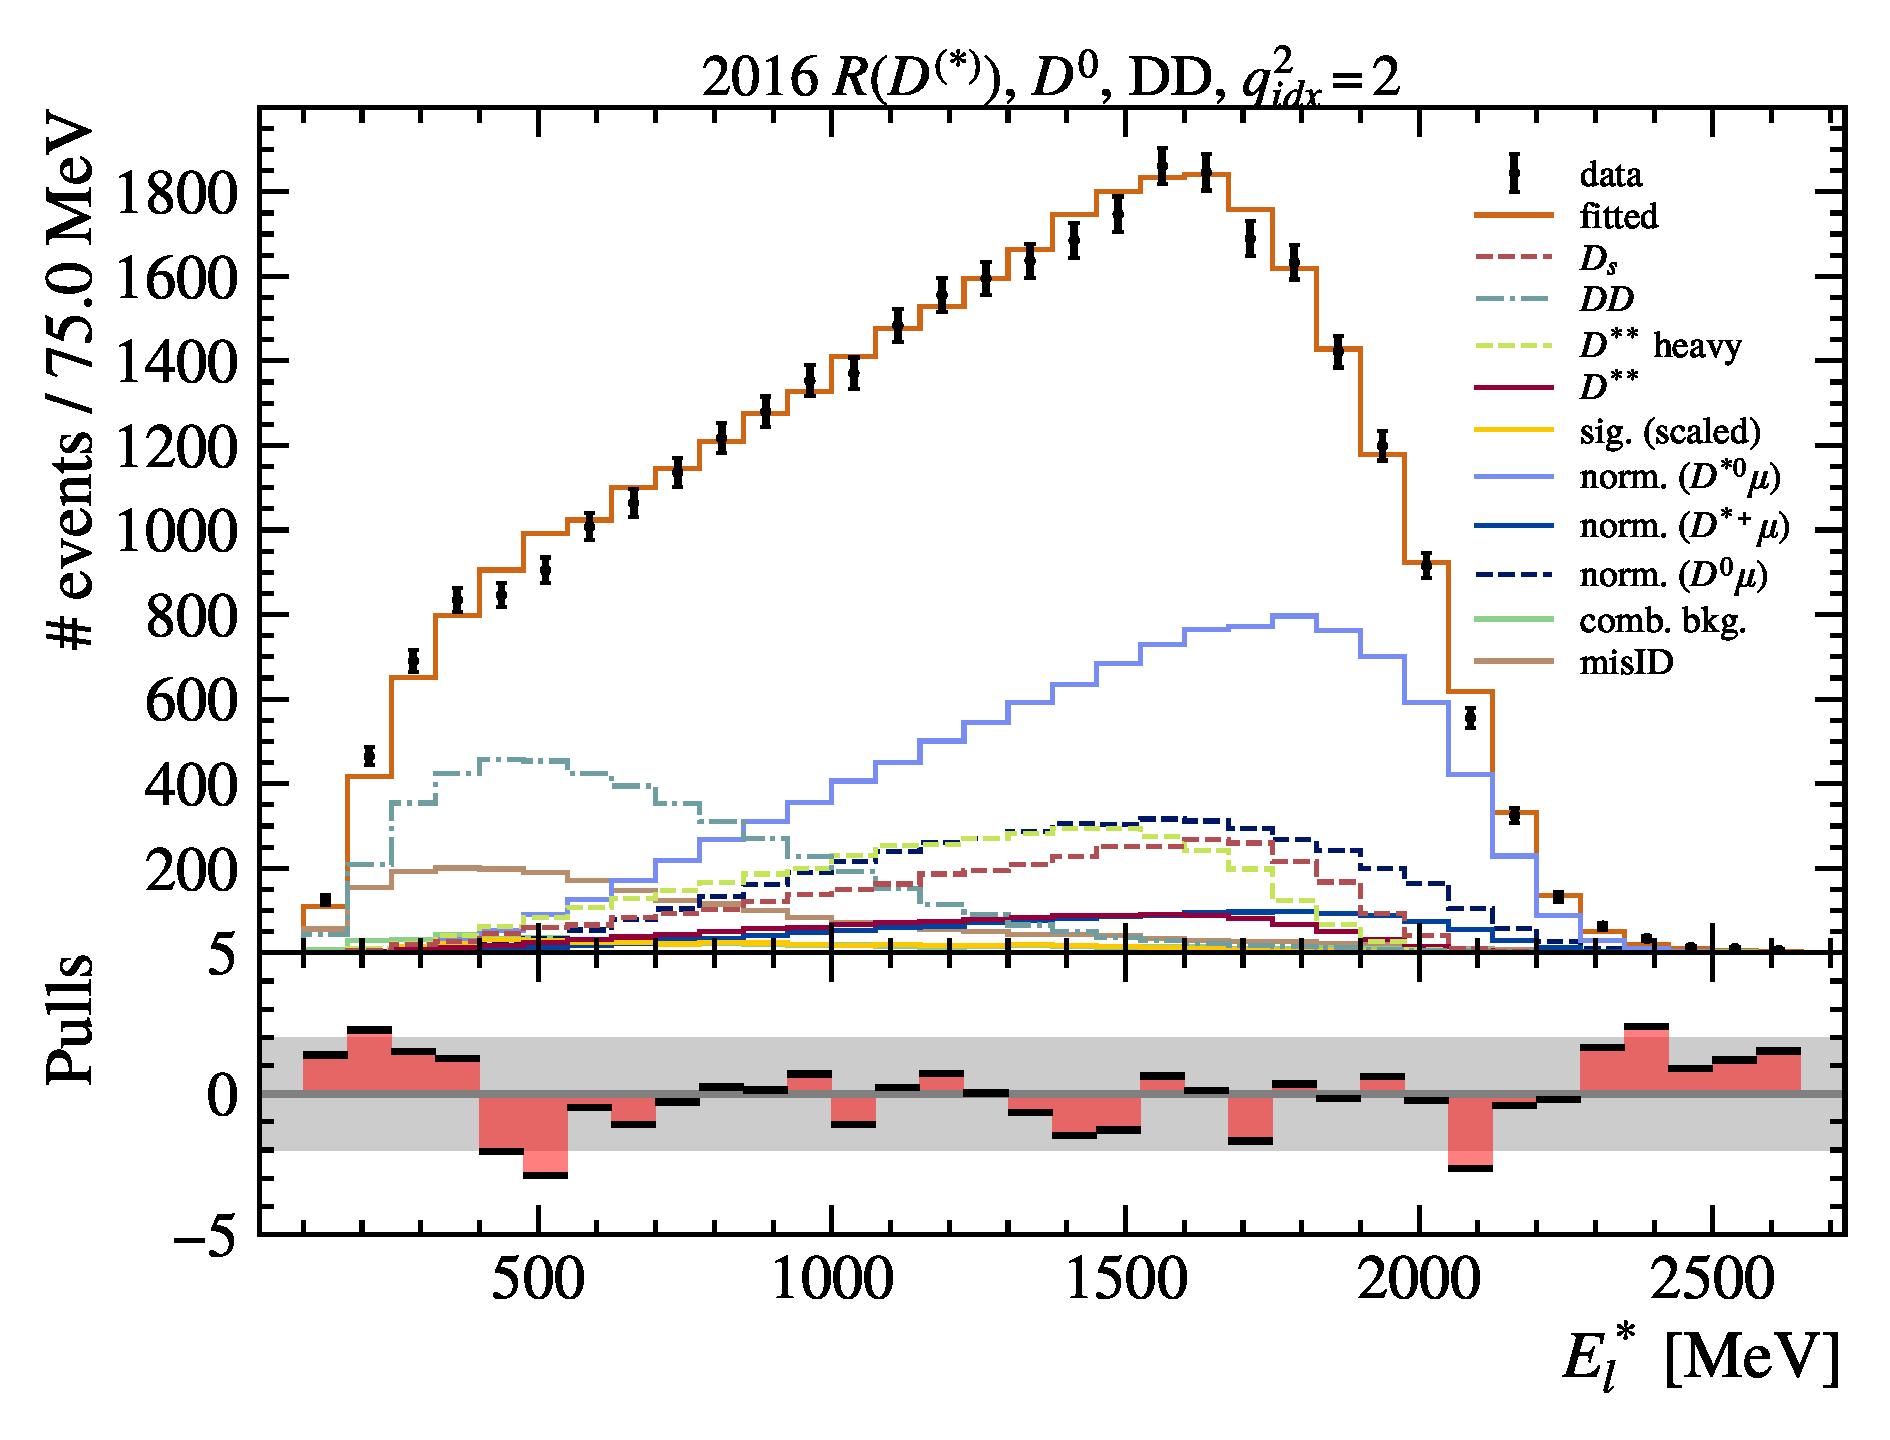
\includegraphics[width=0.24\textwidth]{./figs-fit-fit-results/ctrl-fit/lines_q2_slices/fit_result-lines_q2_idx2-D0-dd-el.pdf}
    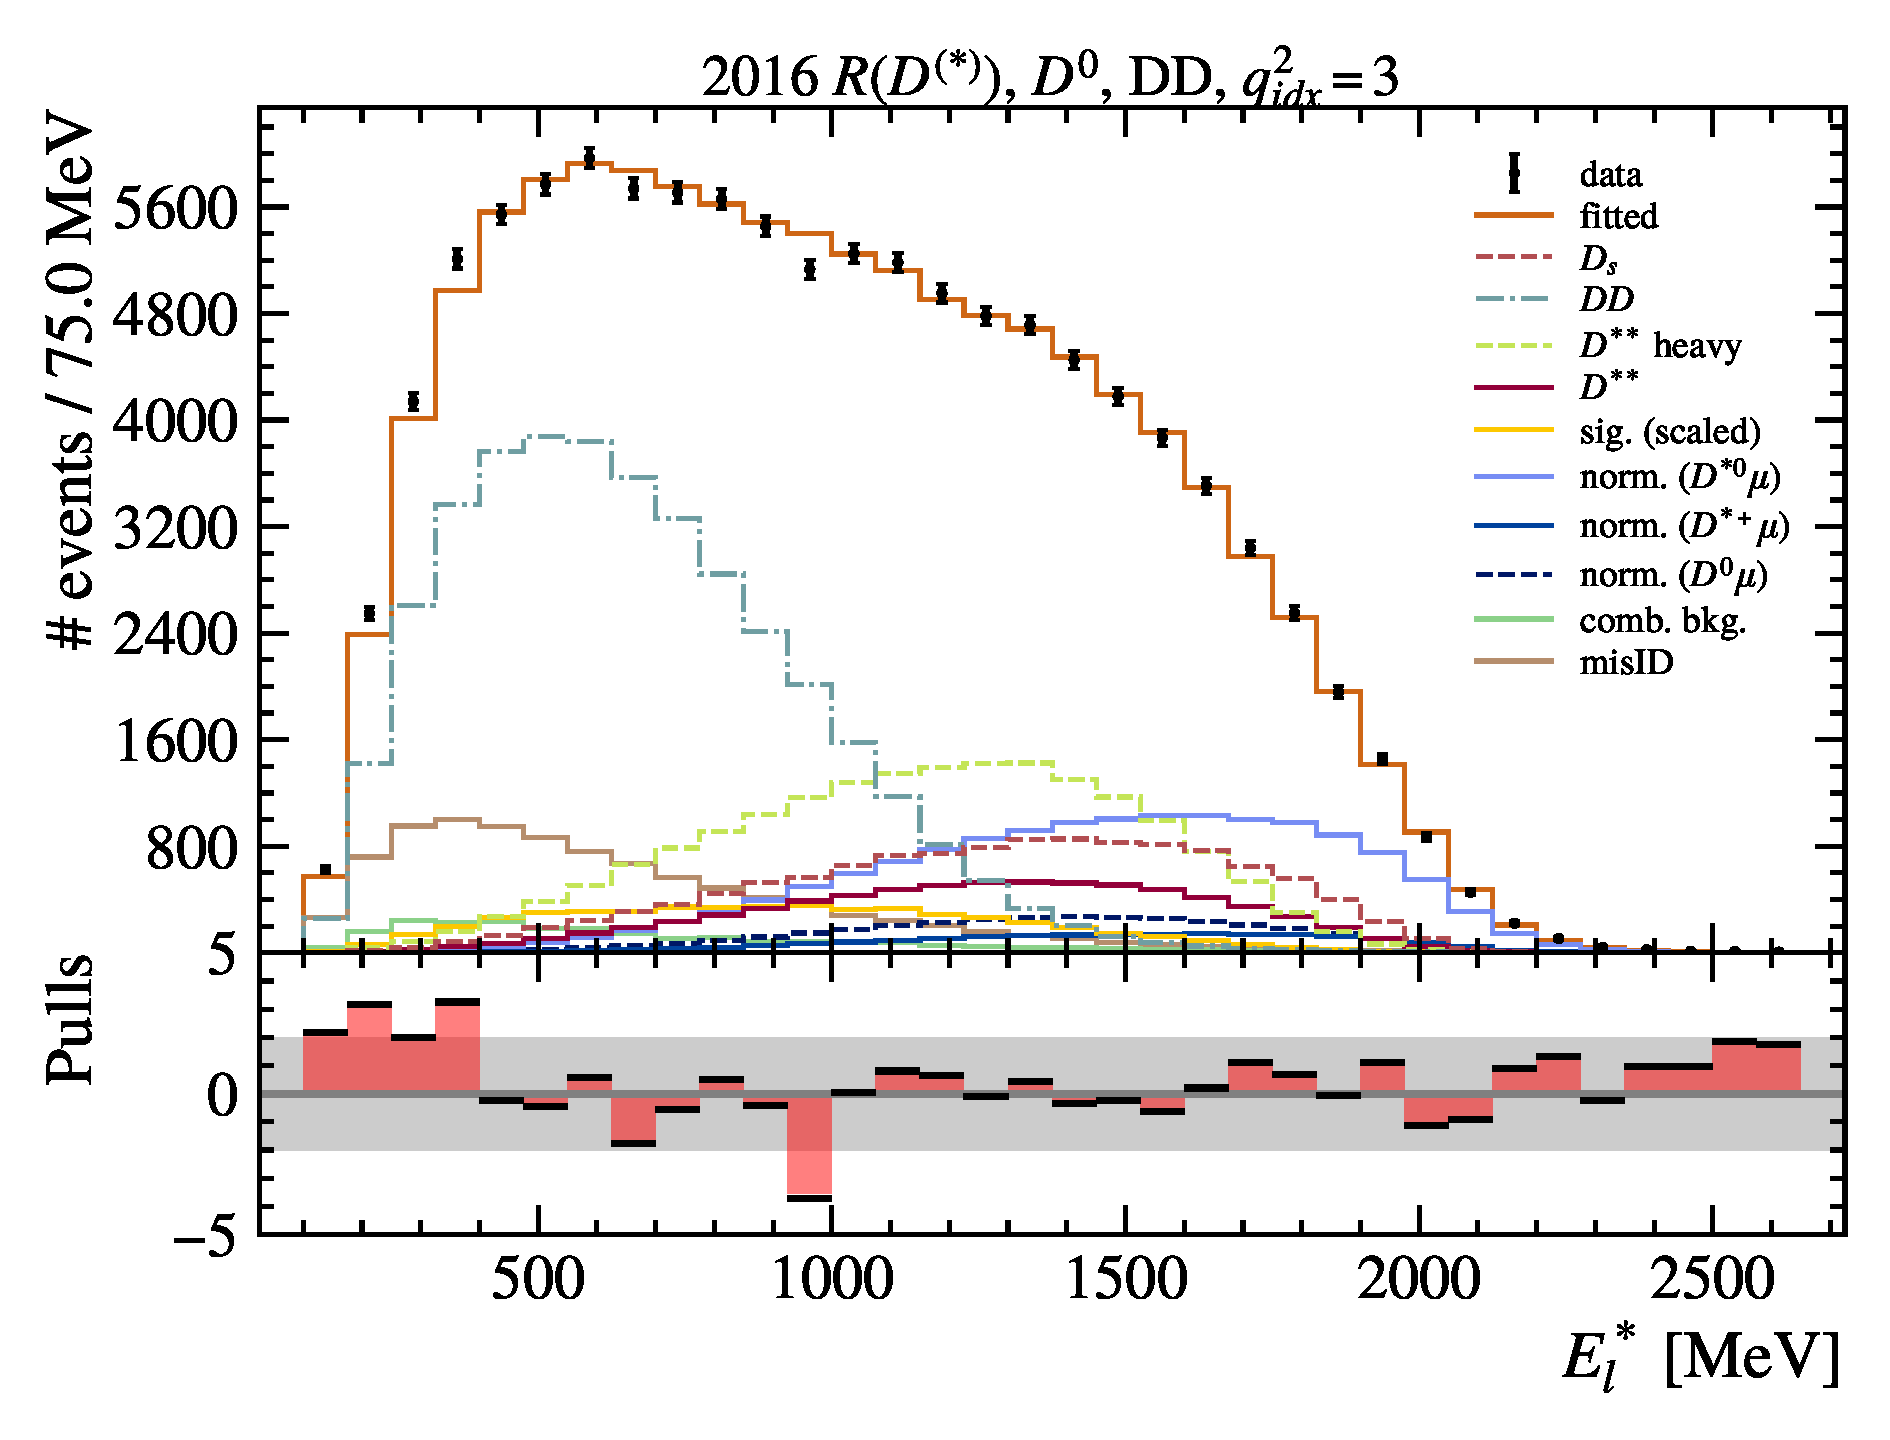
\includegraphics[width=0.24\textwidth]{./figs-fit-fit-results/ctrl-fit/lines_q2_slices/fit_result-lines_q2_idx3-D0-dd-el.pdf}
    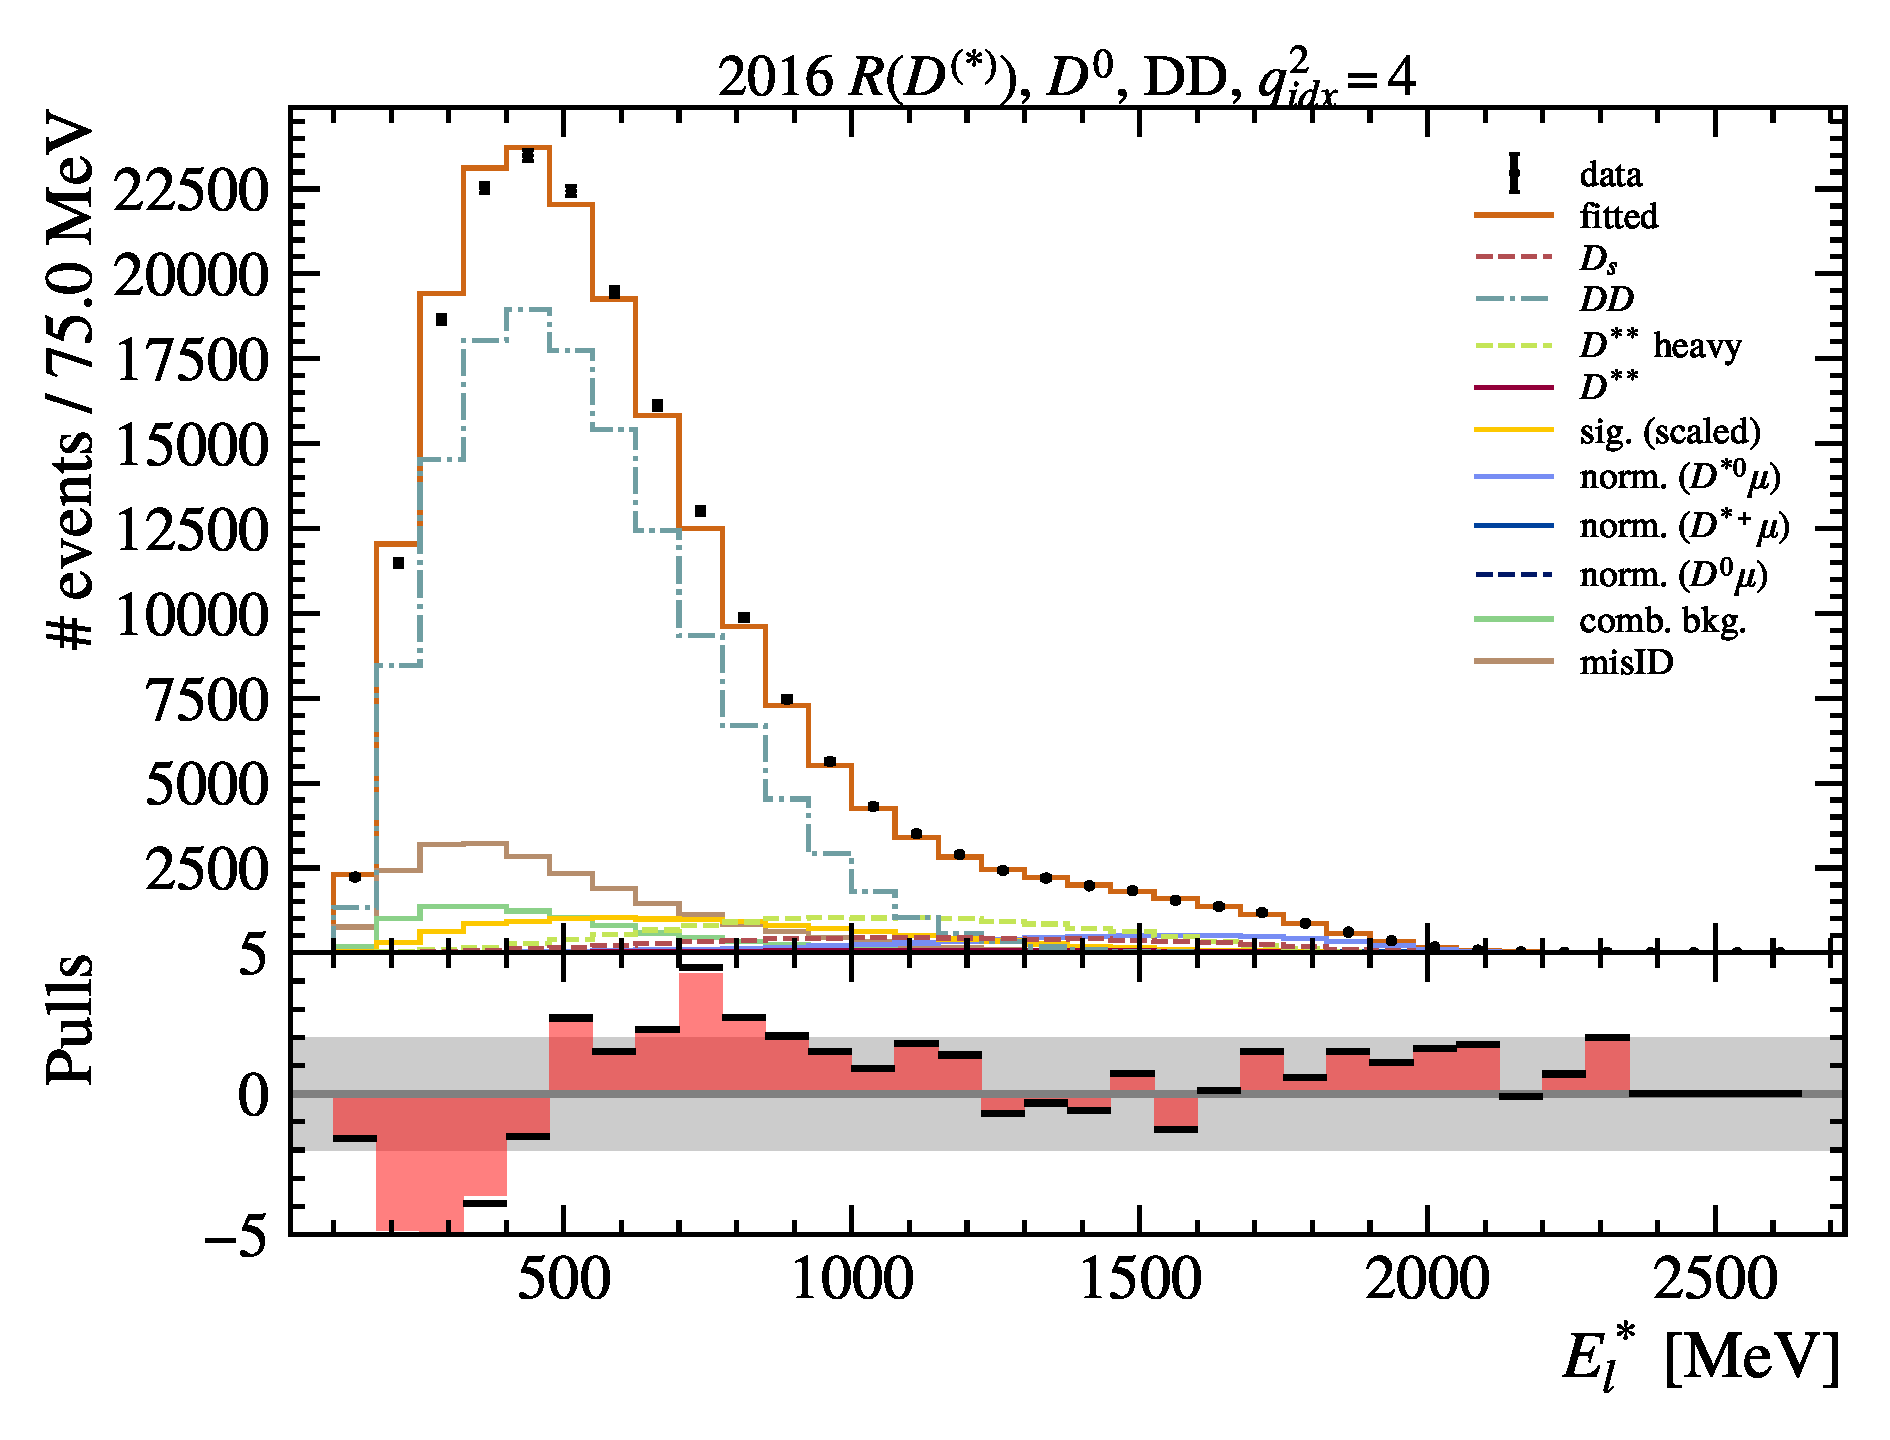
\includegraphics[width=0.24\textwidth]{./figs-fit-fit-results/ctrl-fit/lines_q2_slices/fit_result-lines_q2_idx4-D0-dd-el.pdf}

    \caption{Control fit for DD sample, \Dz channel.}
    \label{fig:ctrl-dd-d0}
\end{figure}

\begin{figure}[!htb]
    \centering
    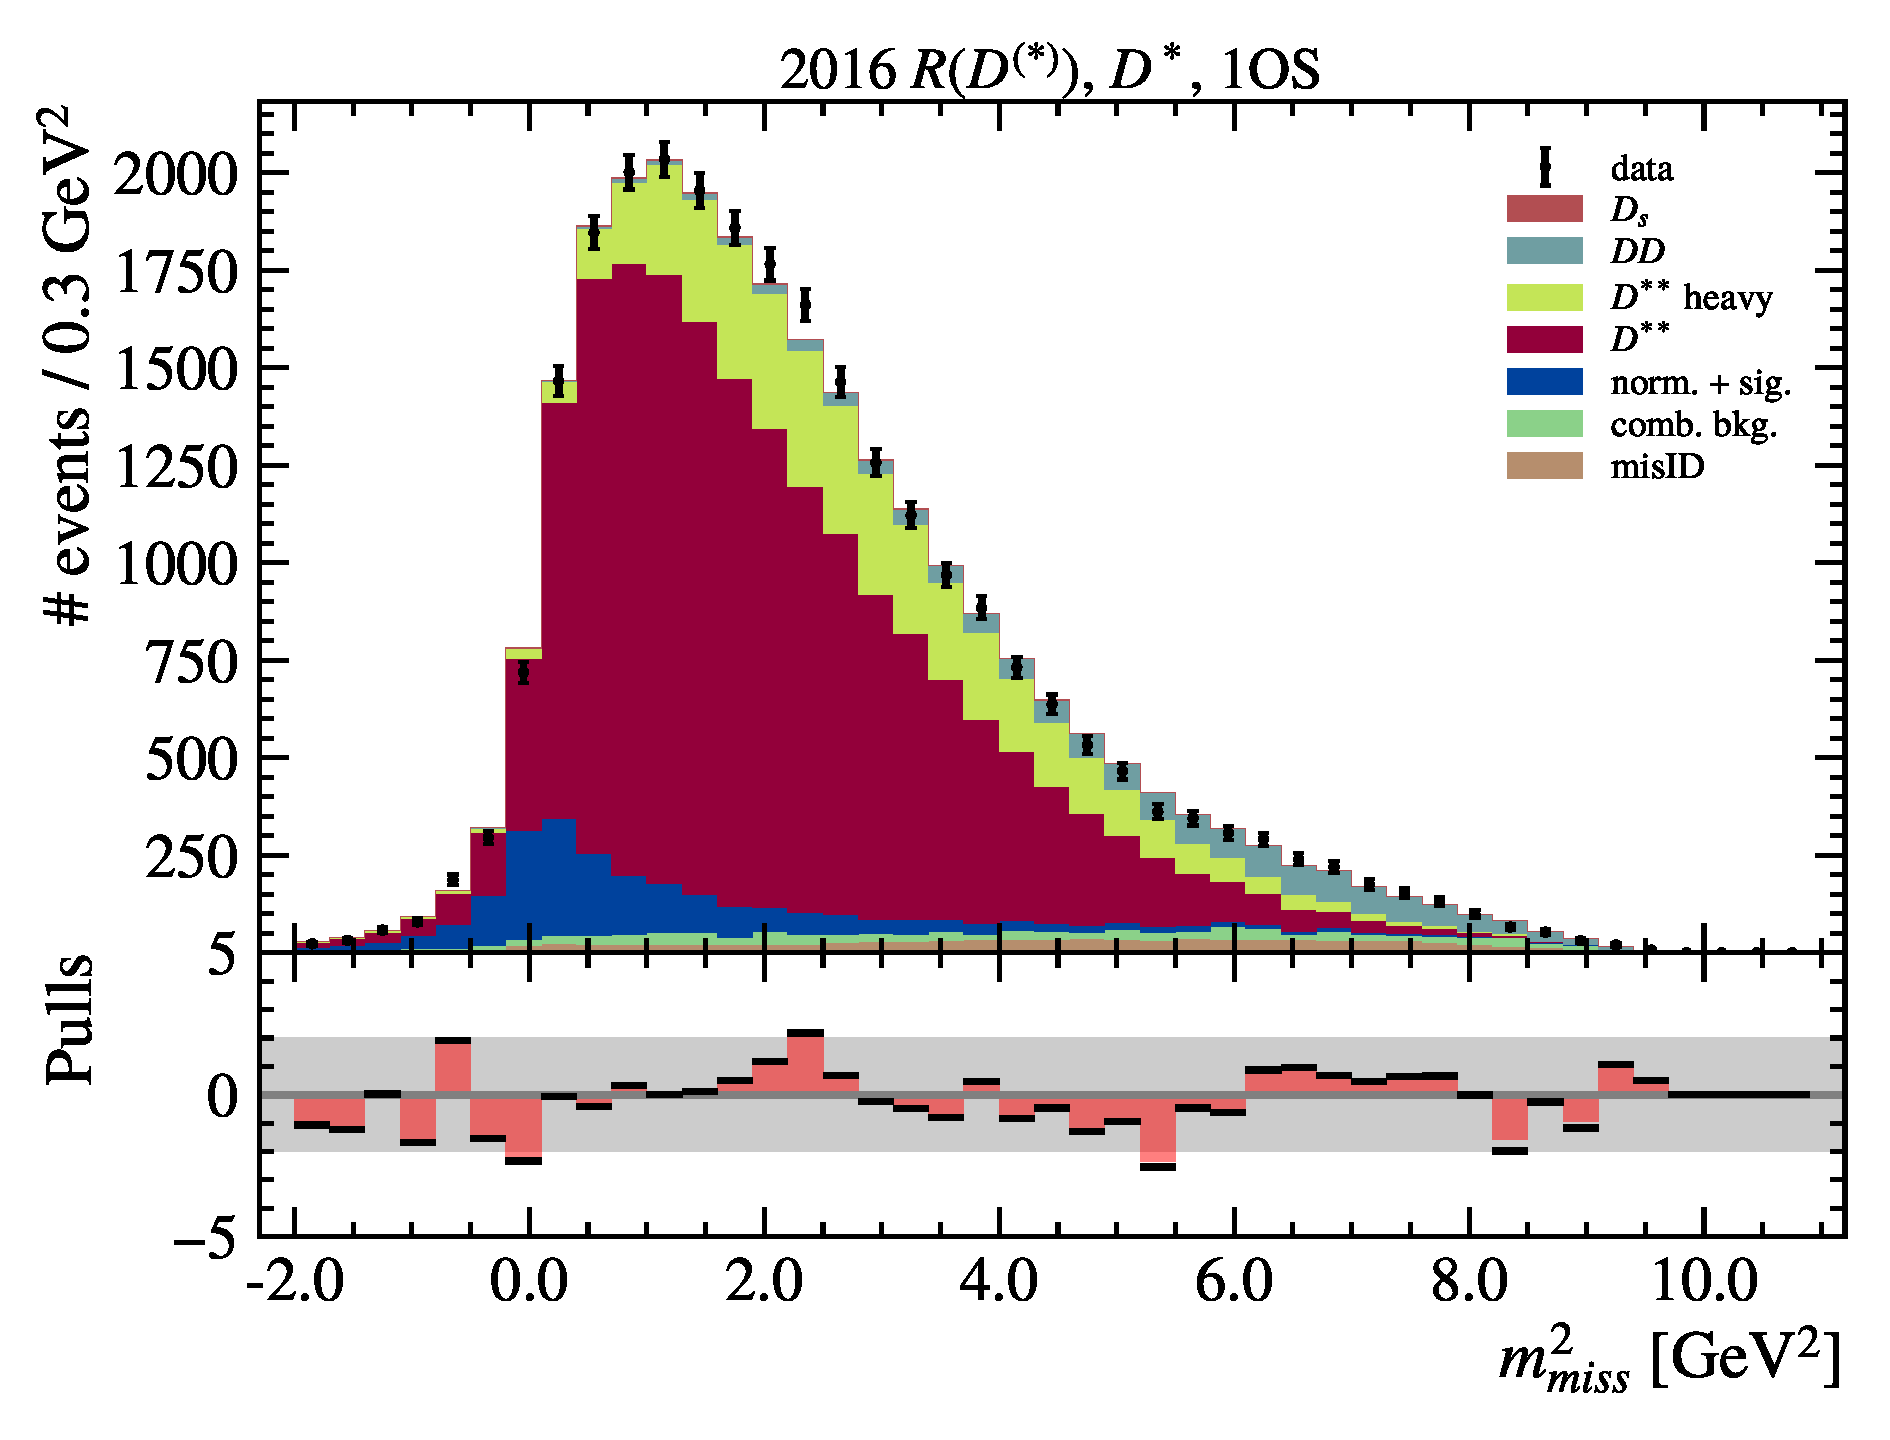
\includegraphics[width=0.32\textwidth]{./figs-fit-fit-results/ctrl-fit/stacked/fit_result-stacked-Dst-1os-mmiss2.pdf}
    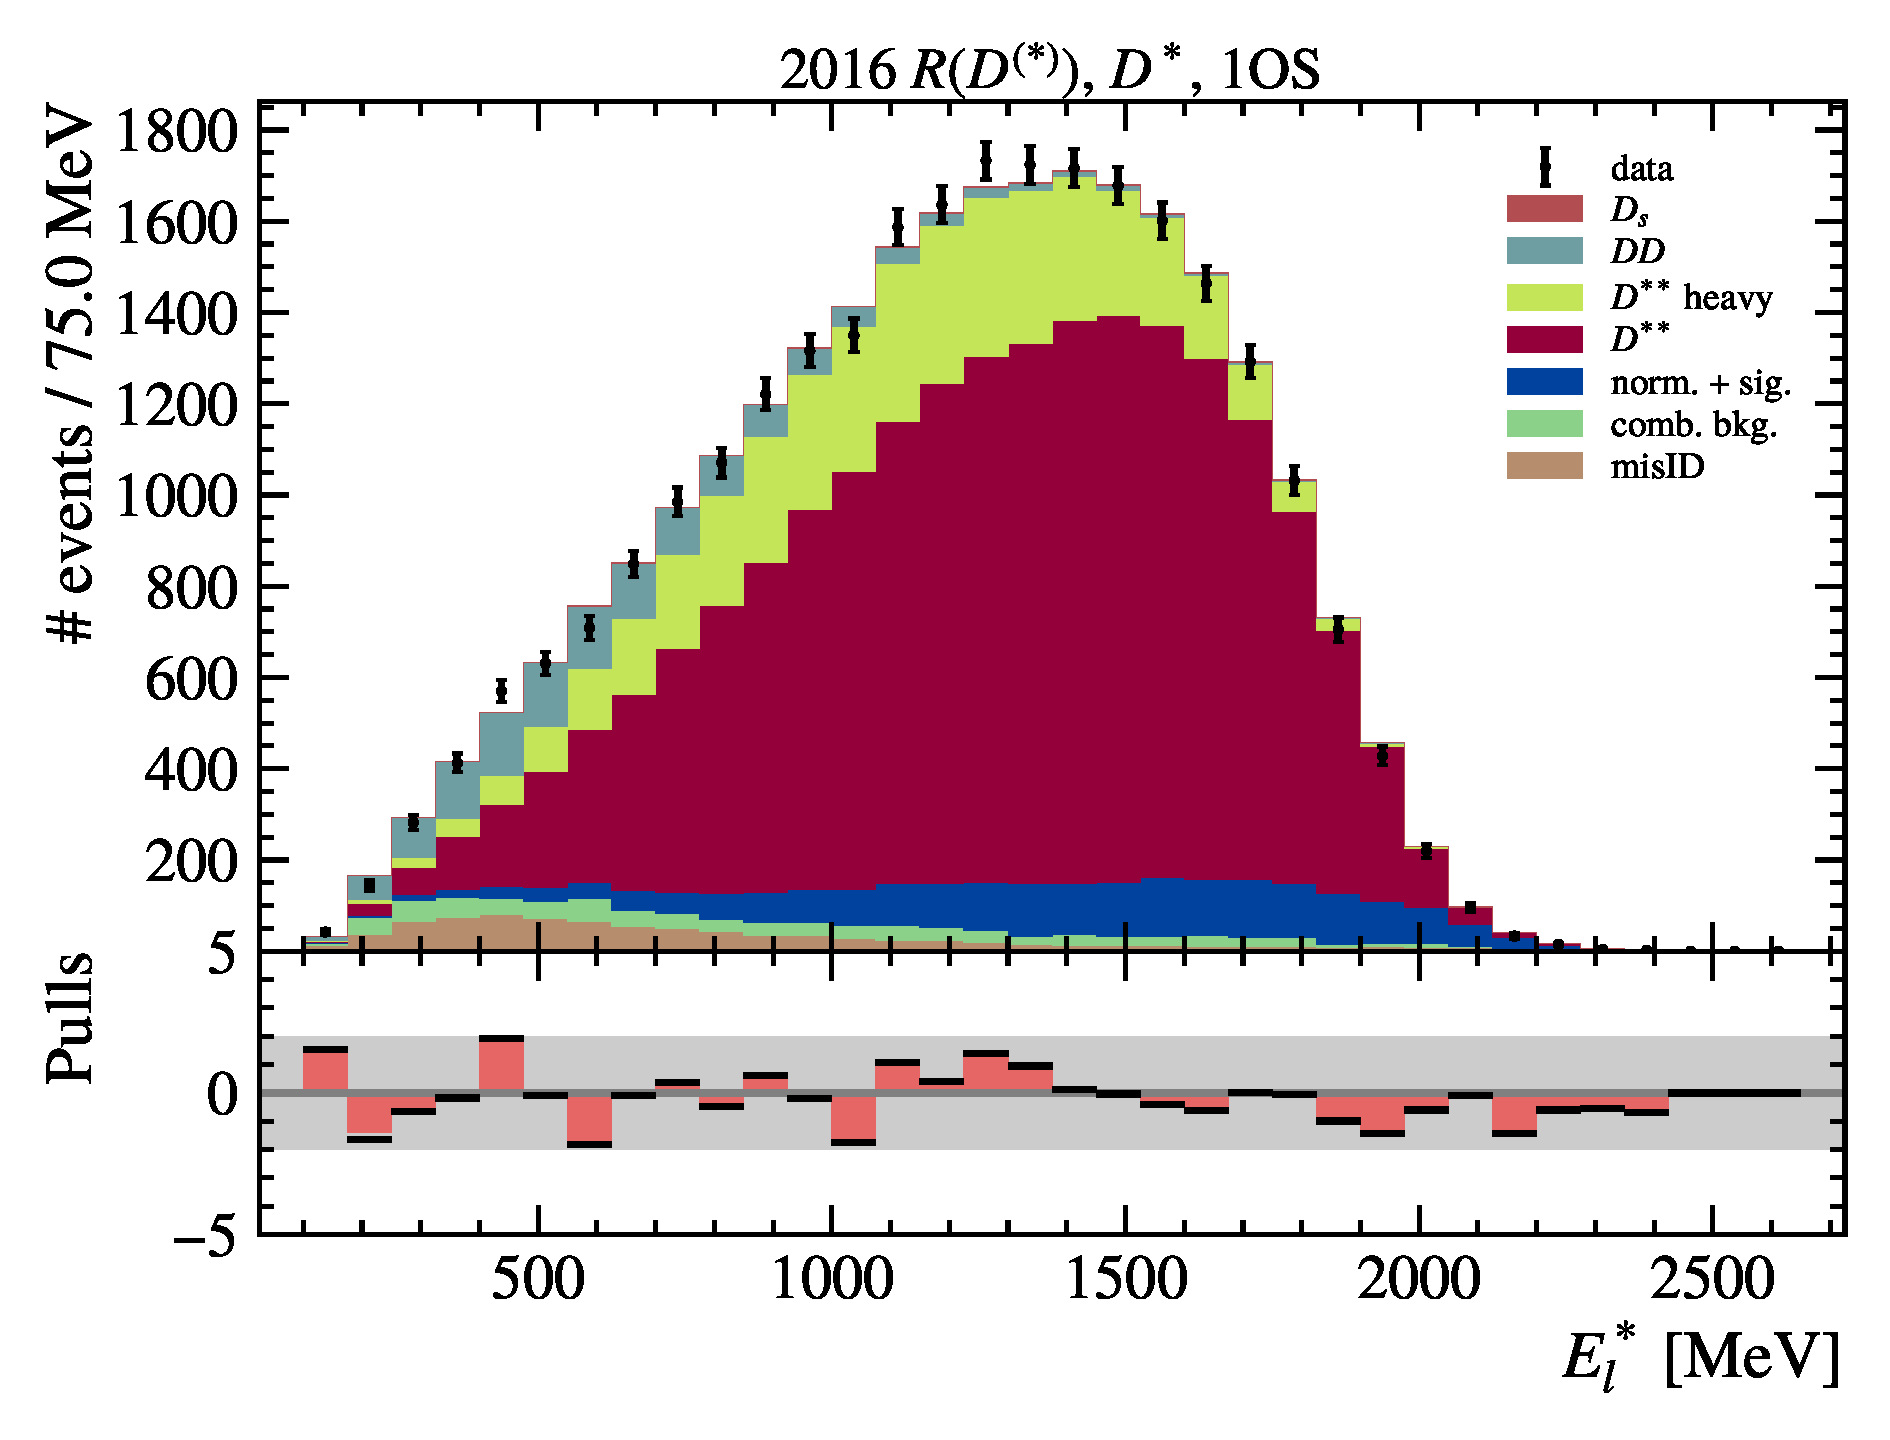
\includegraphics[width=0.32\textwidth]{./figs-fit-fit-results/ctrl-fit/stacked/fit_result-stacked-Dst-1os-el.pdf}
    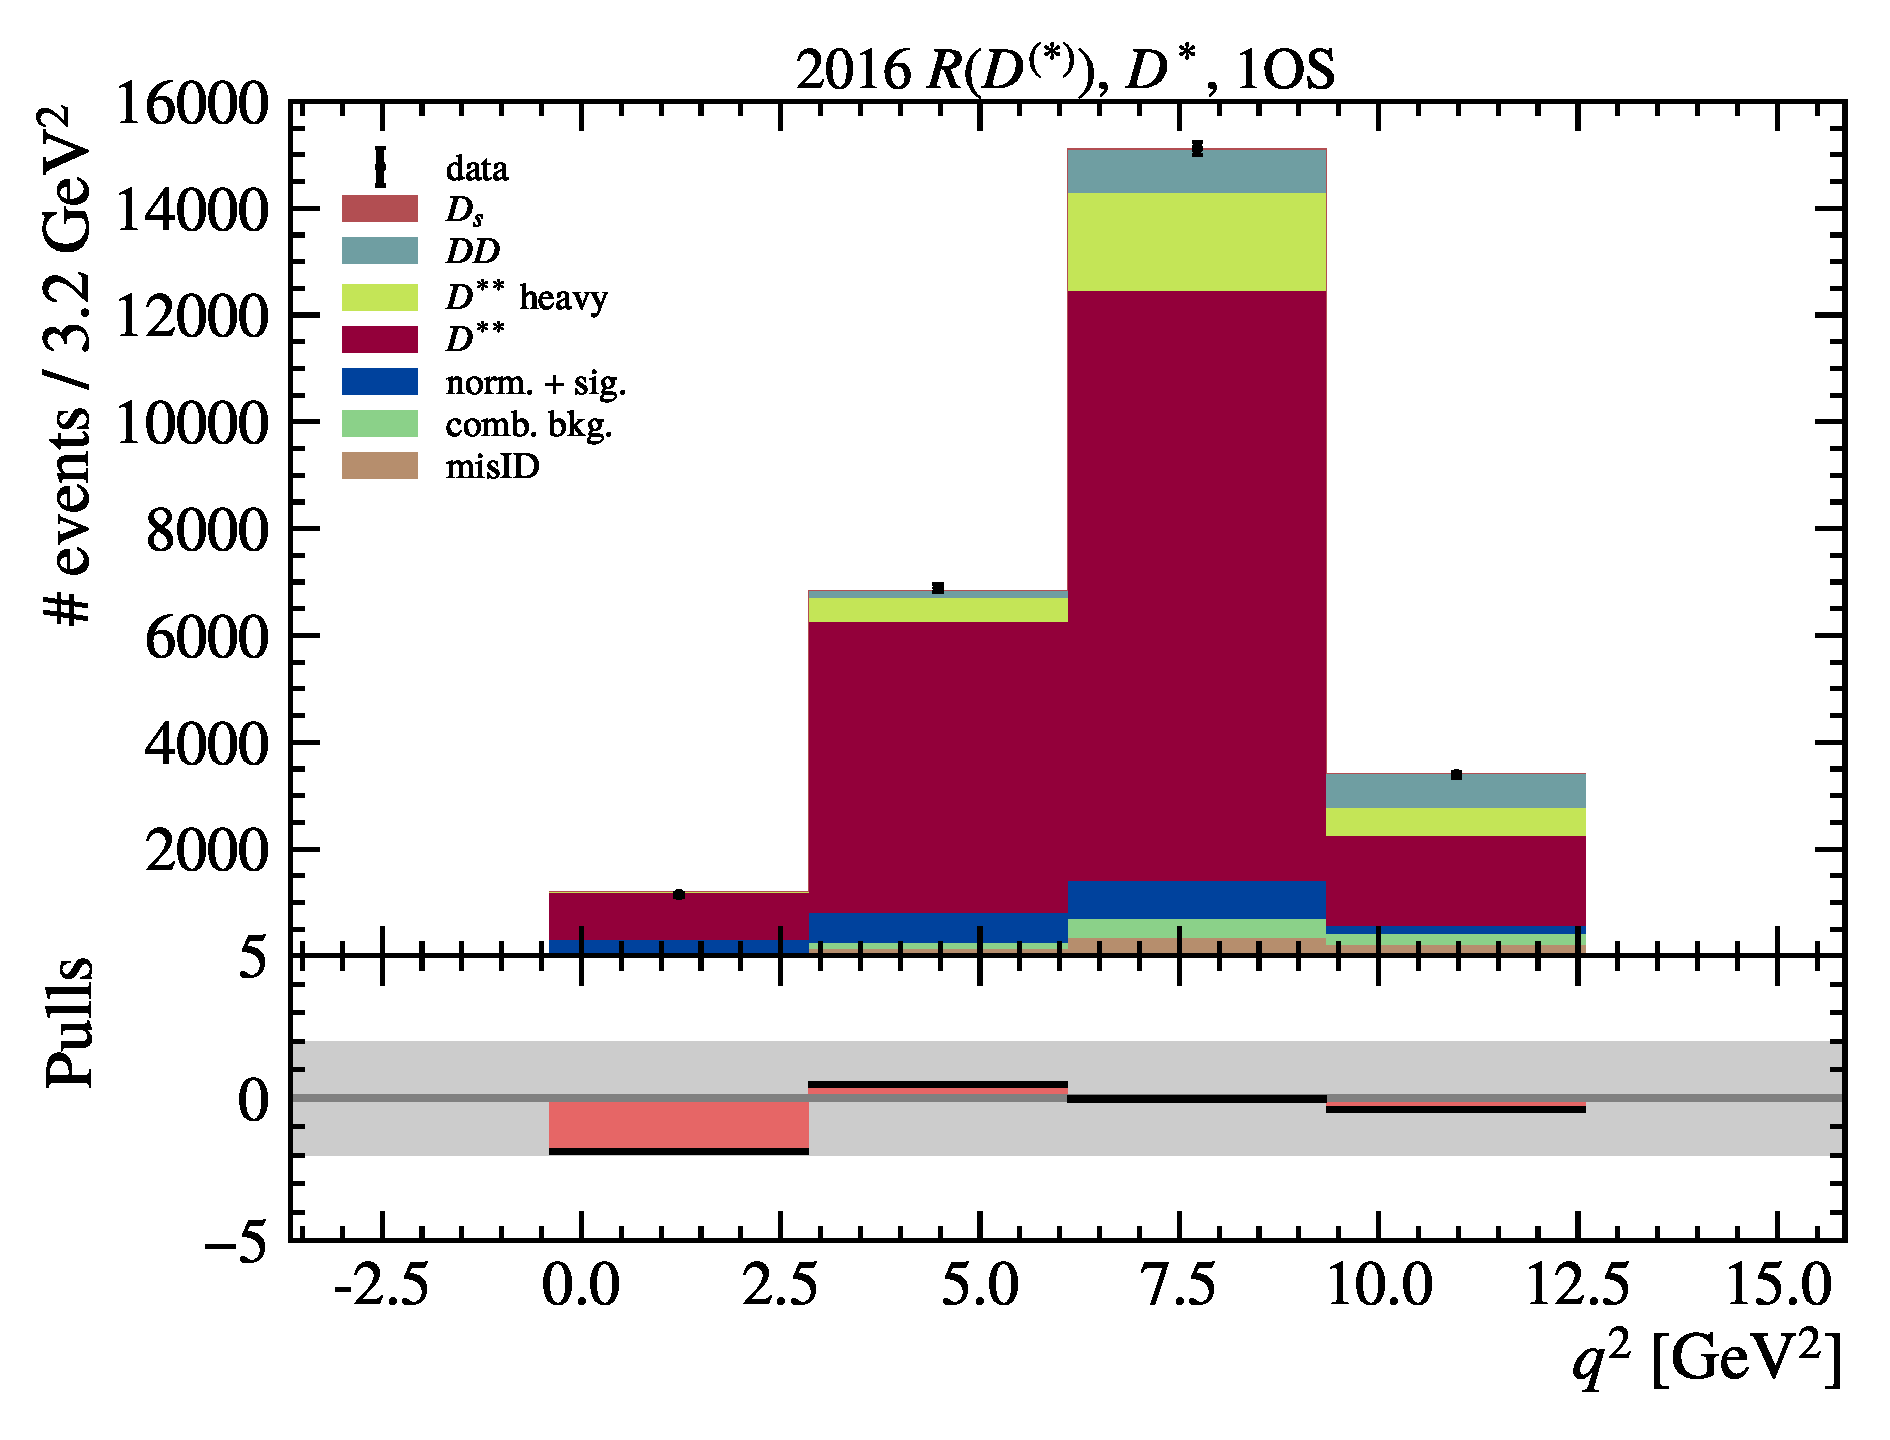
\includegraphics[width=0.32\textwidth]{./figs-fit-fit-results/ctrl-fit/stacked/fit_result-stacked-Dst-1os-q2.pdf}

    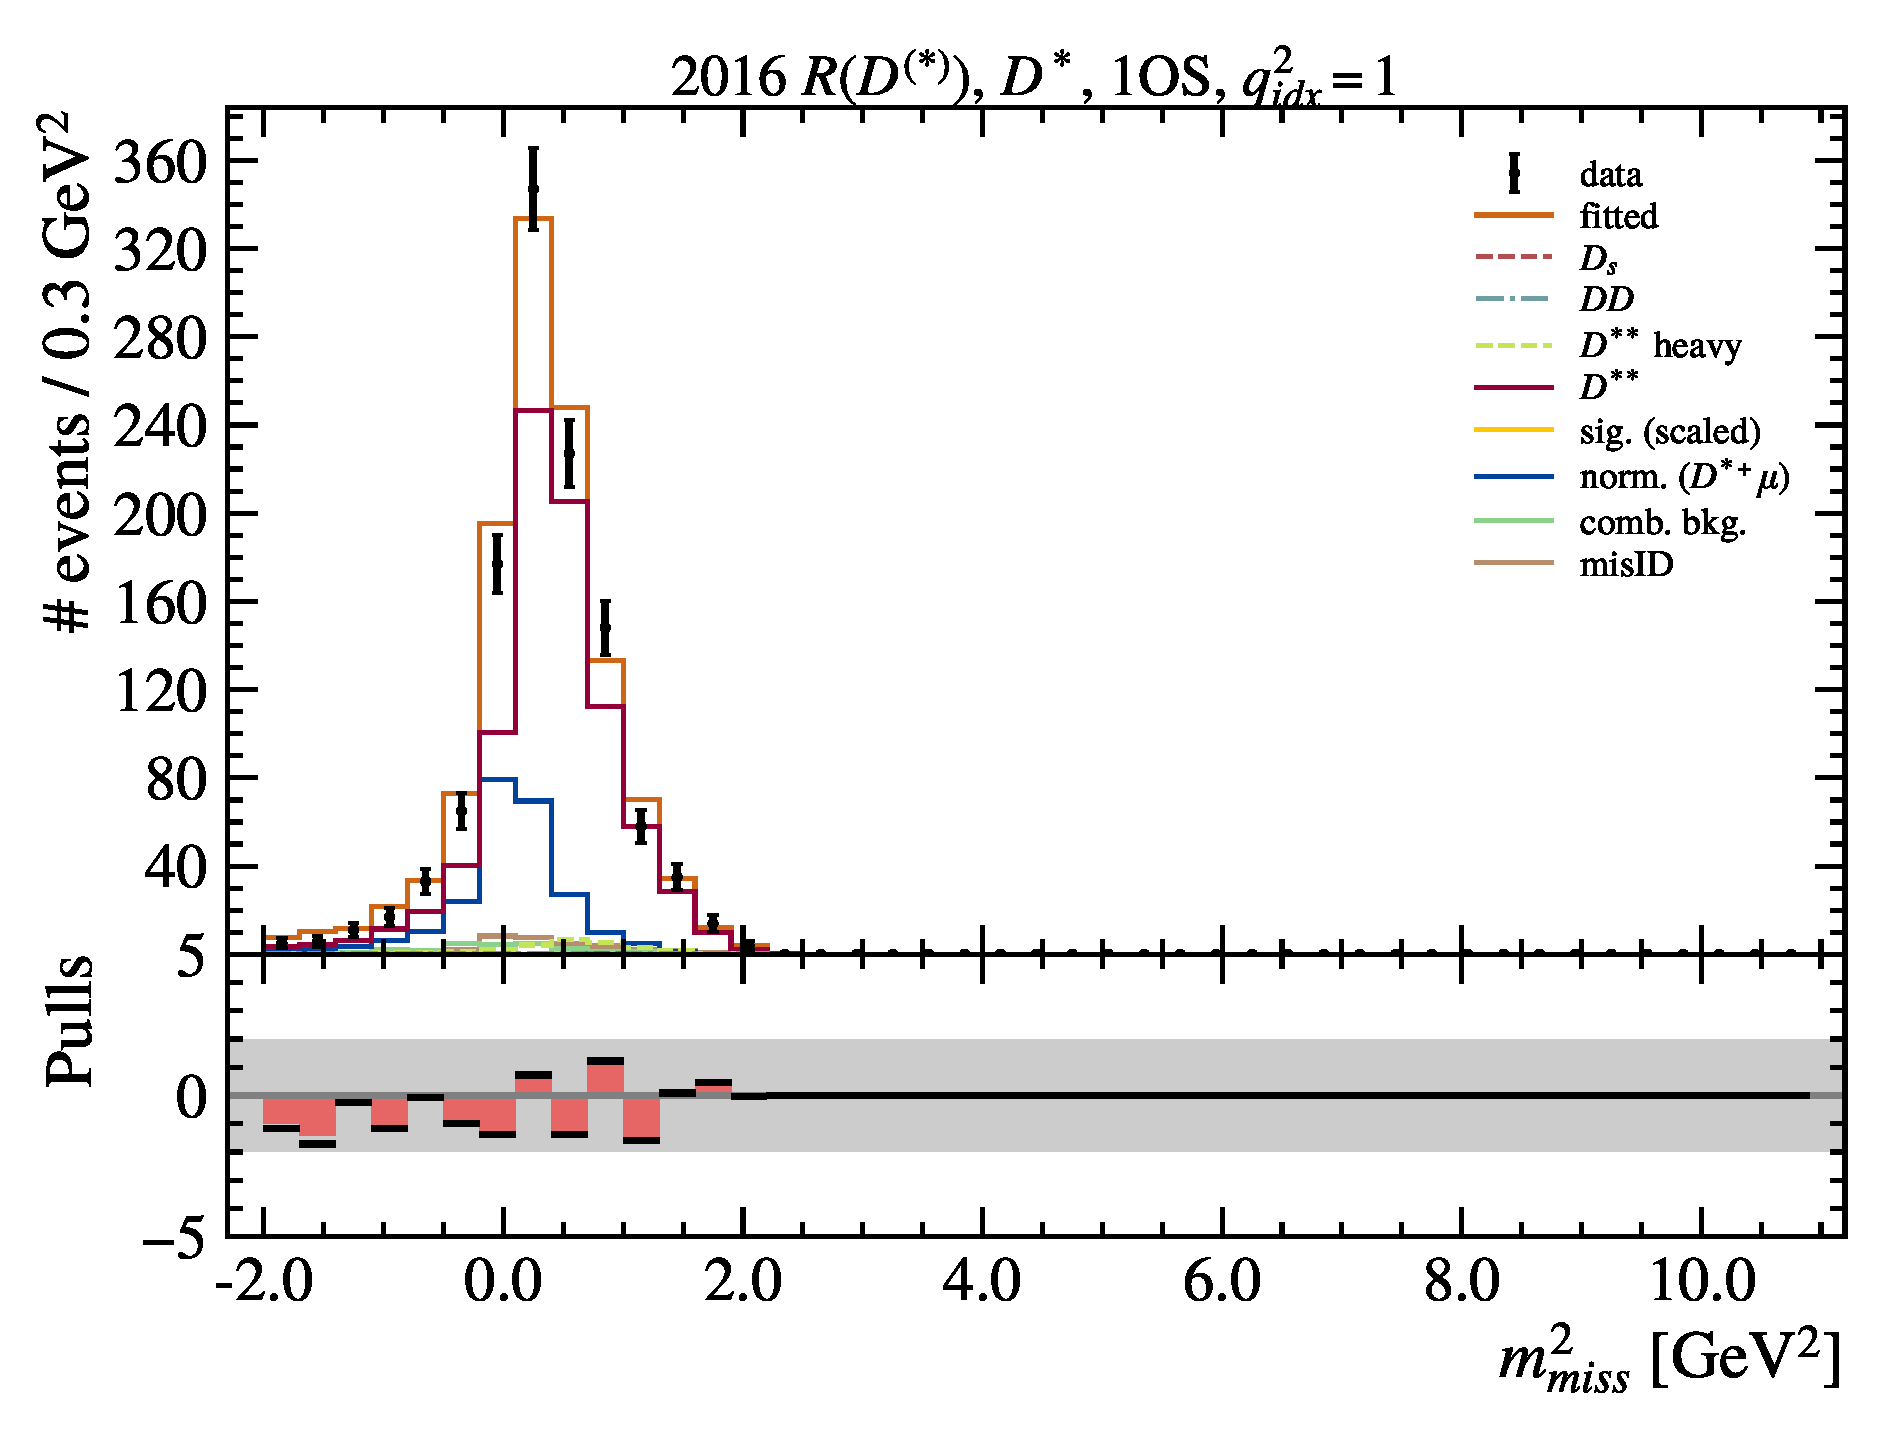
\includegraphics[width=0.24\textwidth]{./figs-fit-fit-results/ctrl-fit/lines_q2_slices/fit_result-lines_q2_idx1-Dst-1os-mmiss2.pdf}
    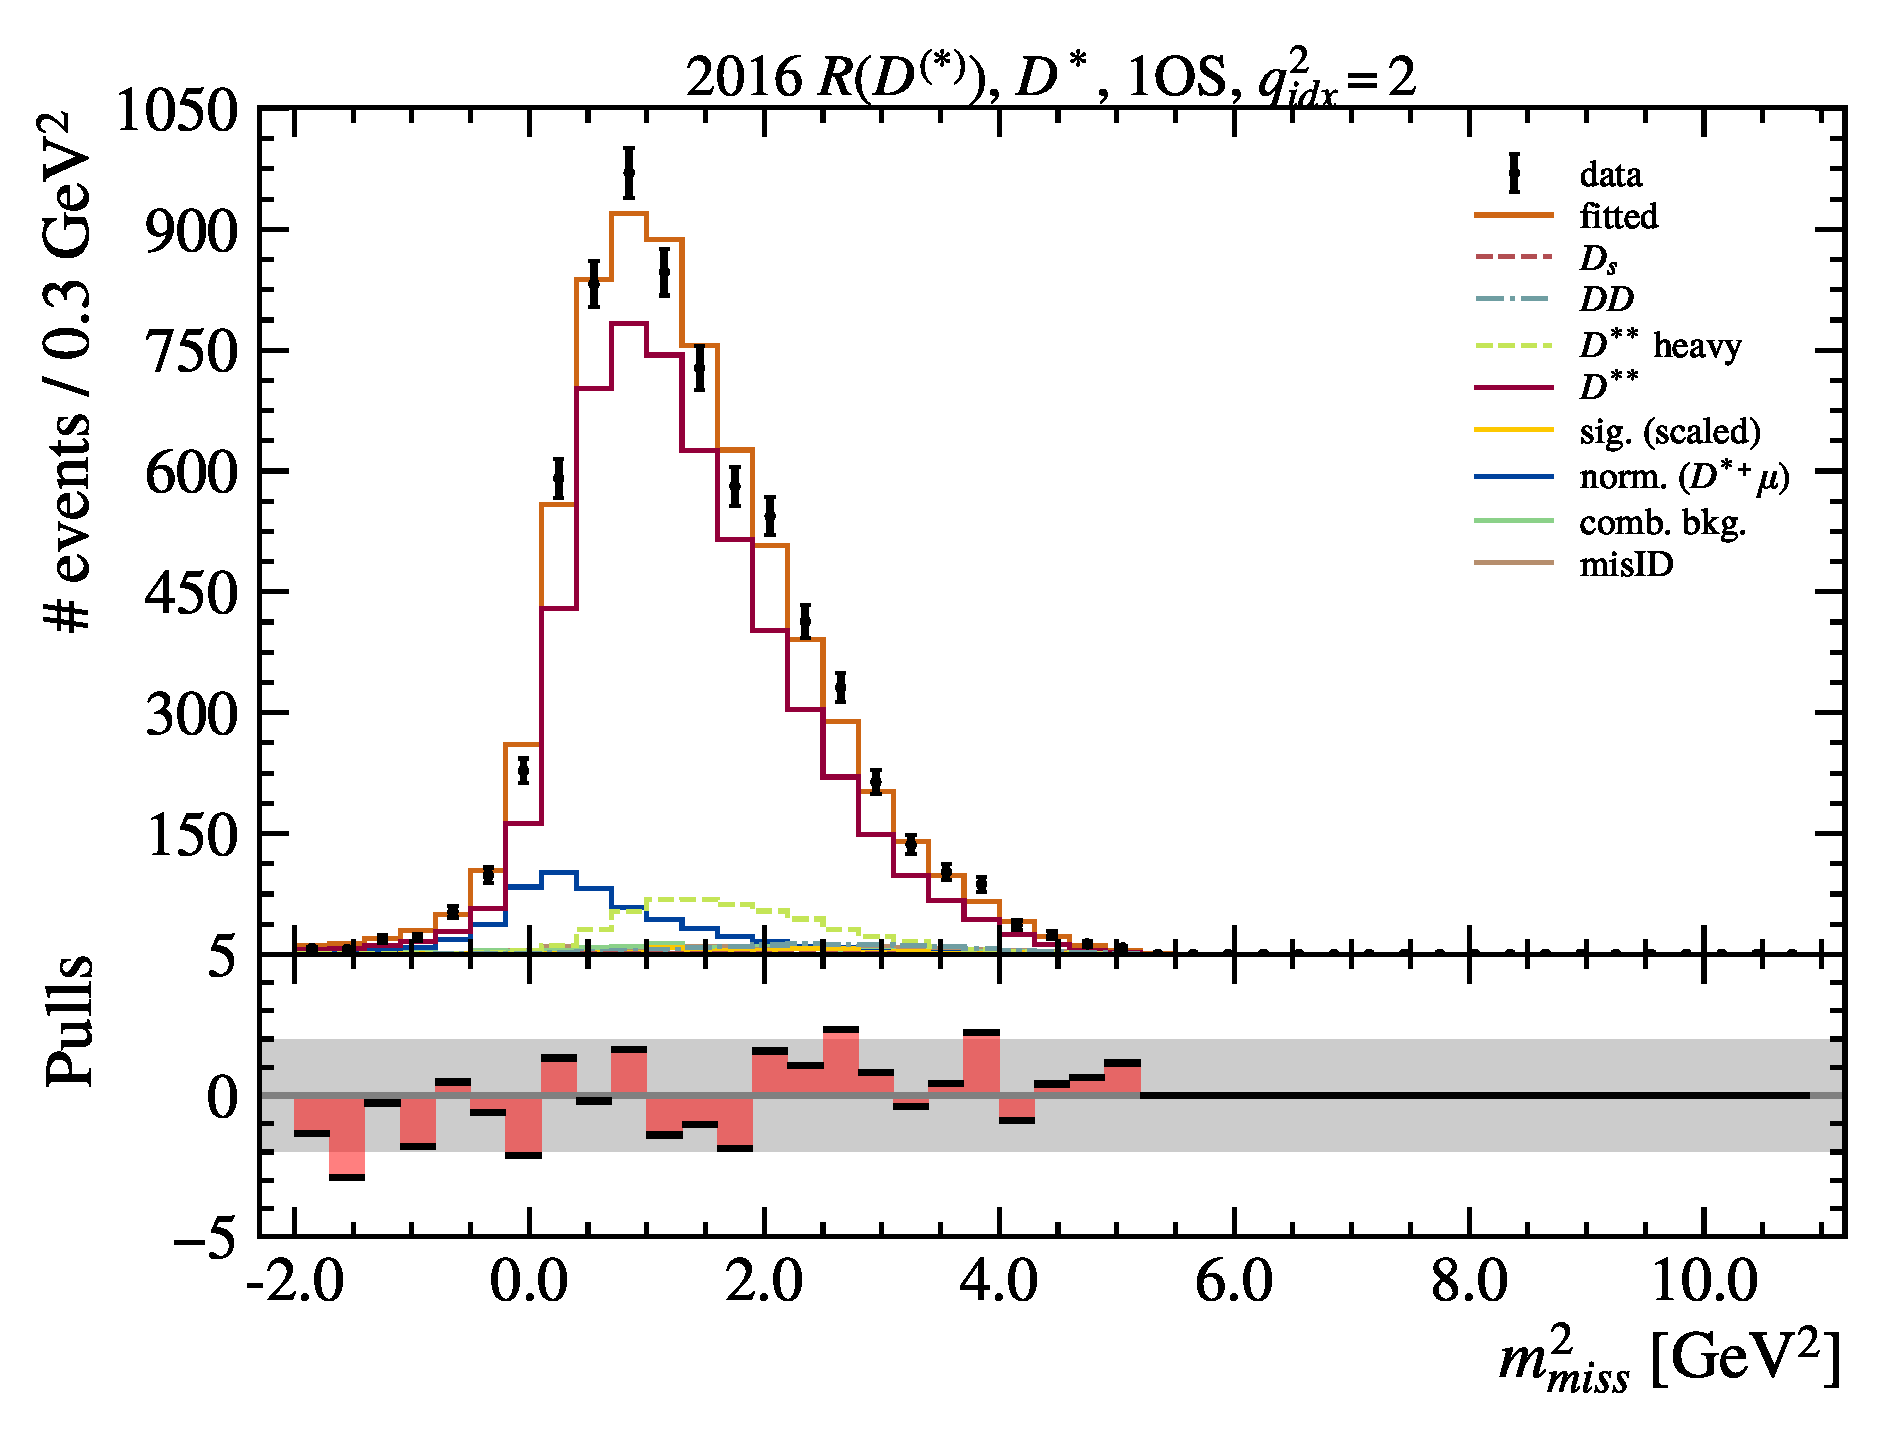
\includegraphics[width=0.24\textwidth]{./figs-fit-fit-results/ctrl-fit/lines_q2_slices/fit_result-lines_q2_idx2-Dst-1os-mmiss2.pdf}
    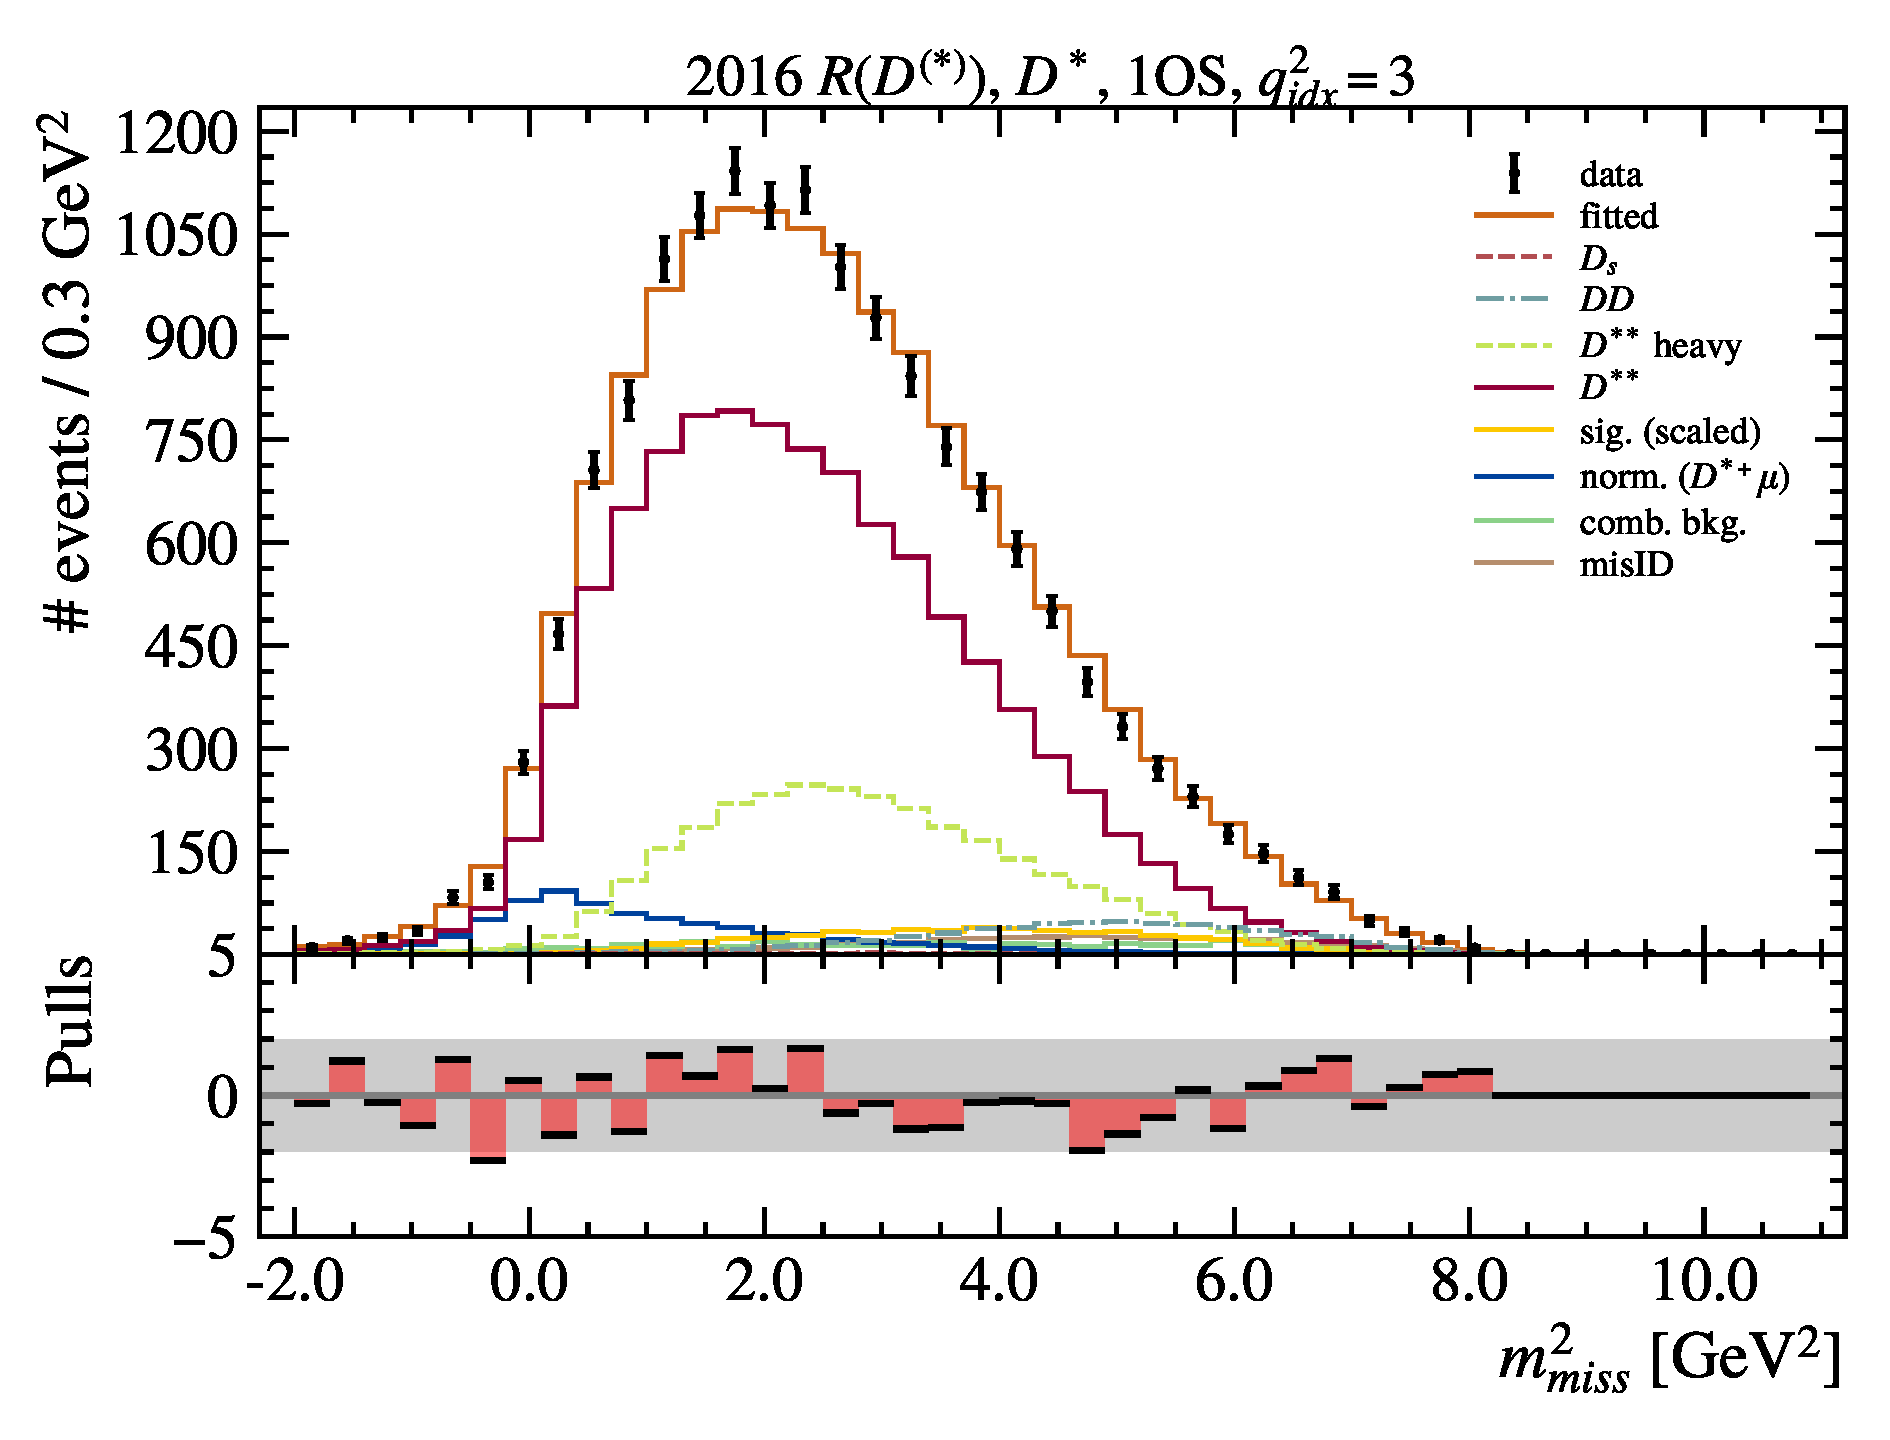
\includegraphics[width=0.24\textwidth]{./figs-fit-fit-results/ctrl-fit/lines_q2_slices/fit_result-lines_q2_idx3-Dst-1os-mmiss2.pdf}
    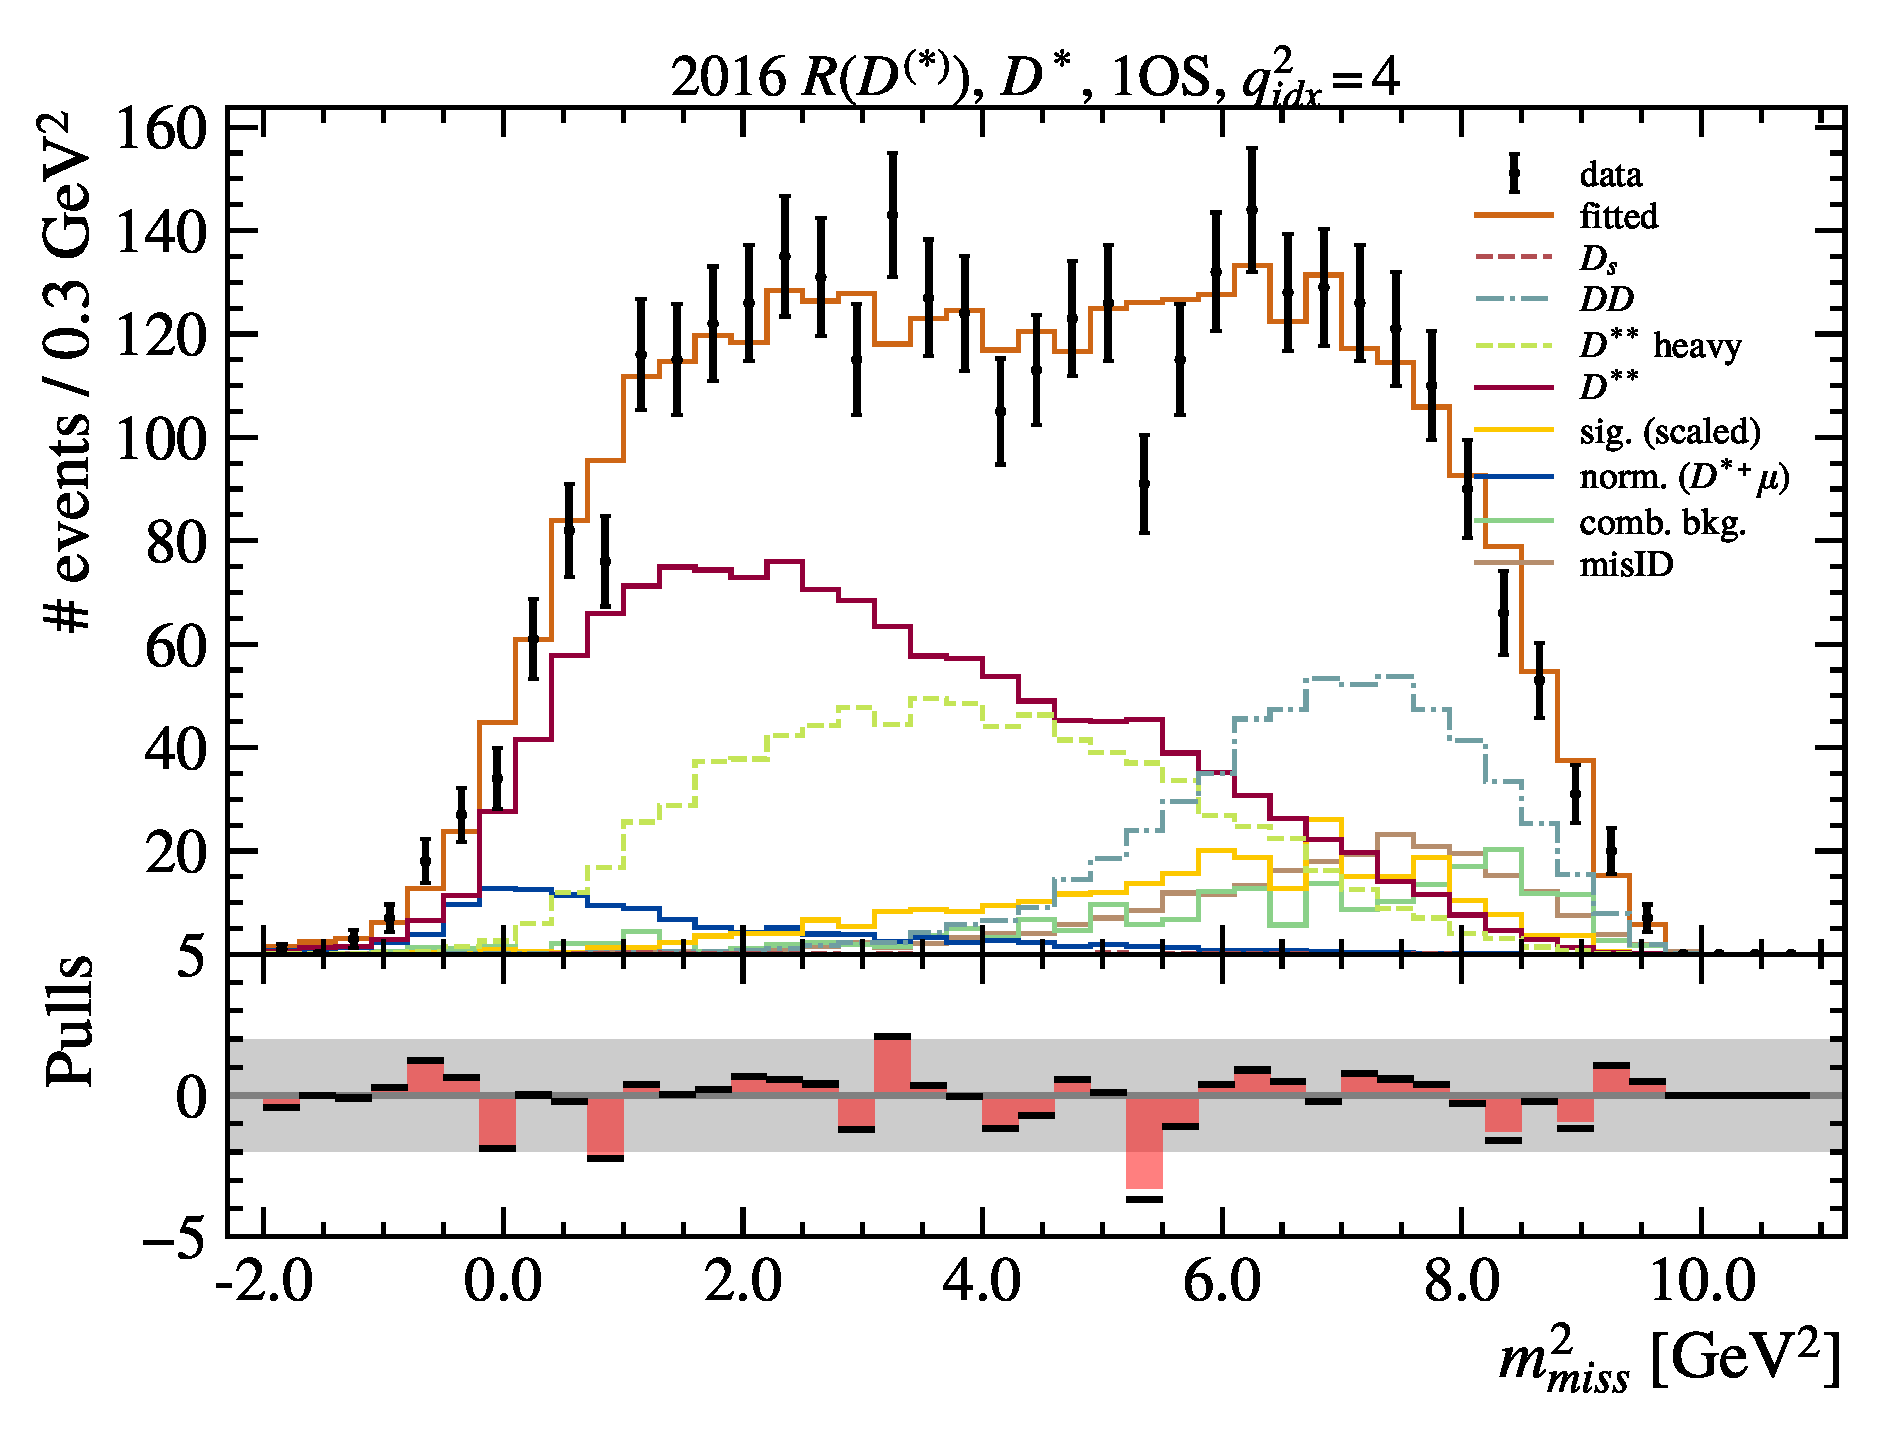
\includegraphics[width=0.24\textwidth]{./figs-fit-fit-results/ctrl-fit/lines_q2_slices/fit_result-lines_q2_idx4-Dst-1os-mmiss2.pdf}

    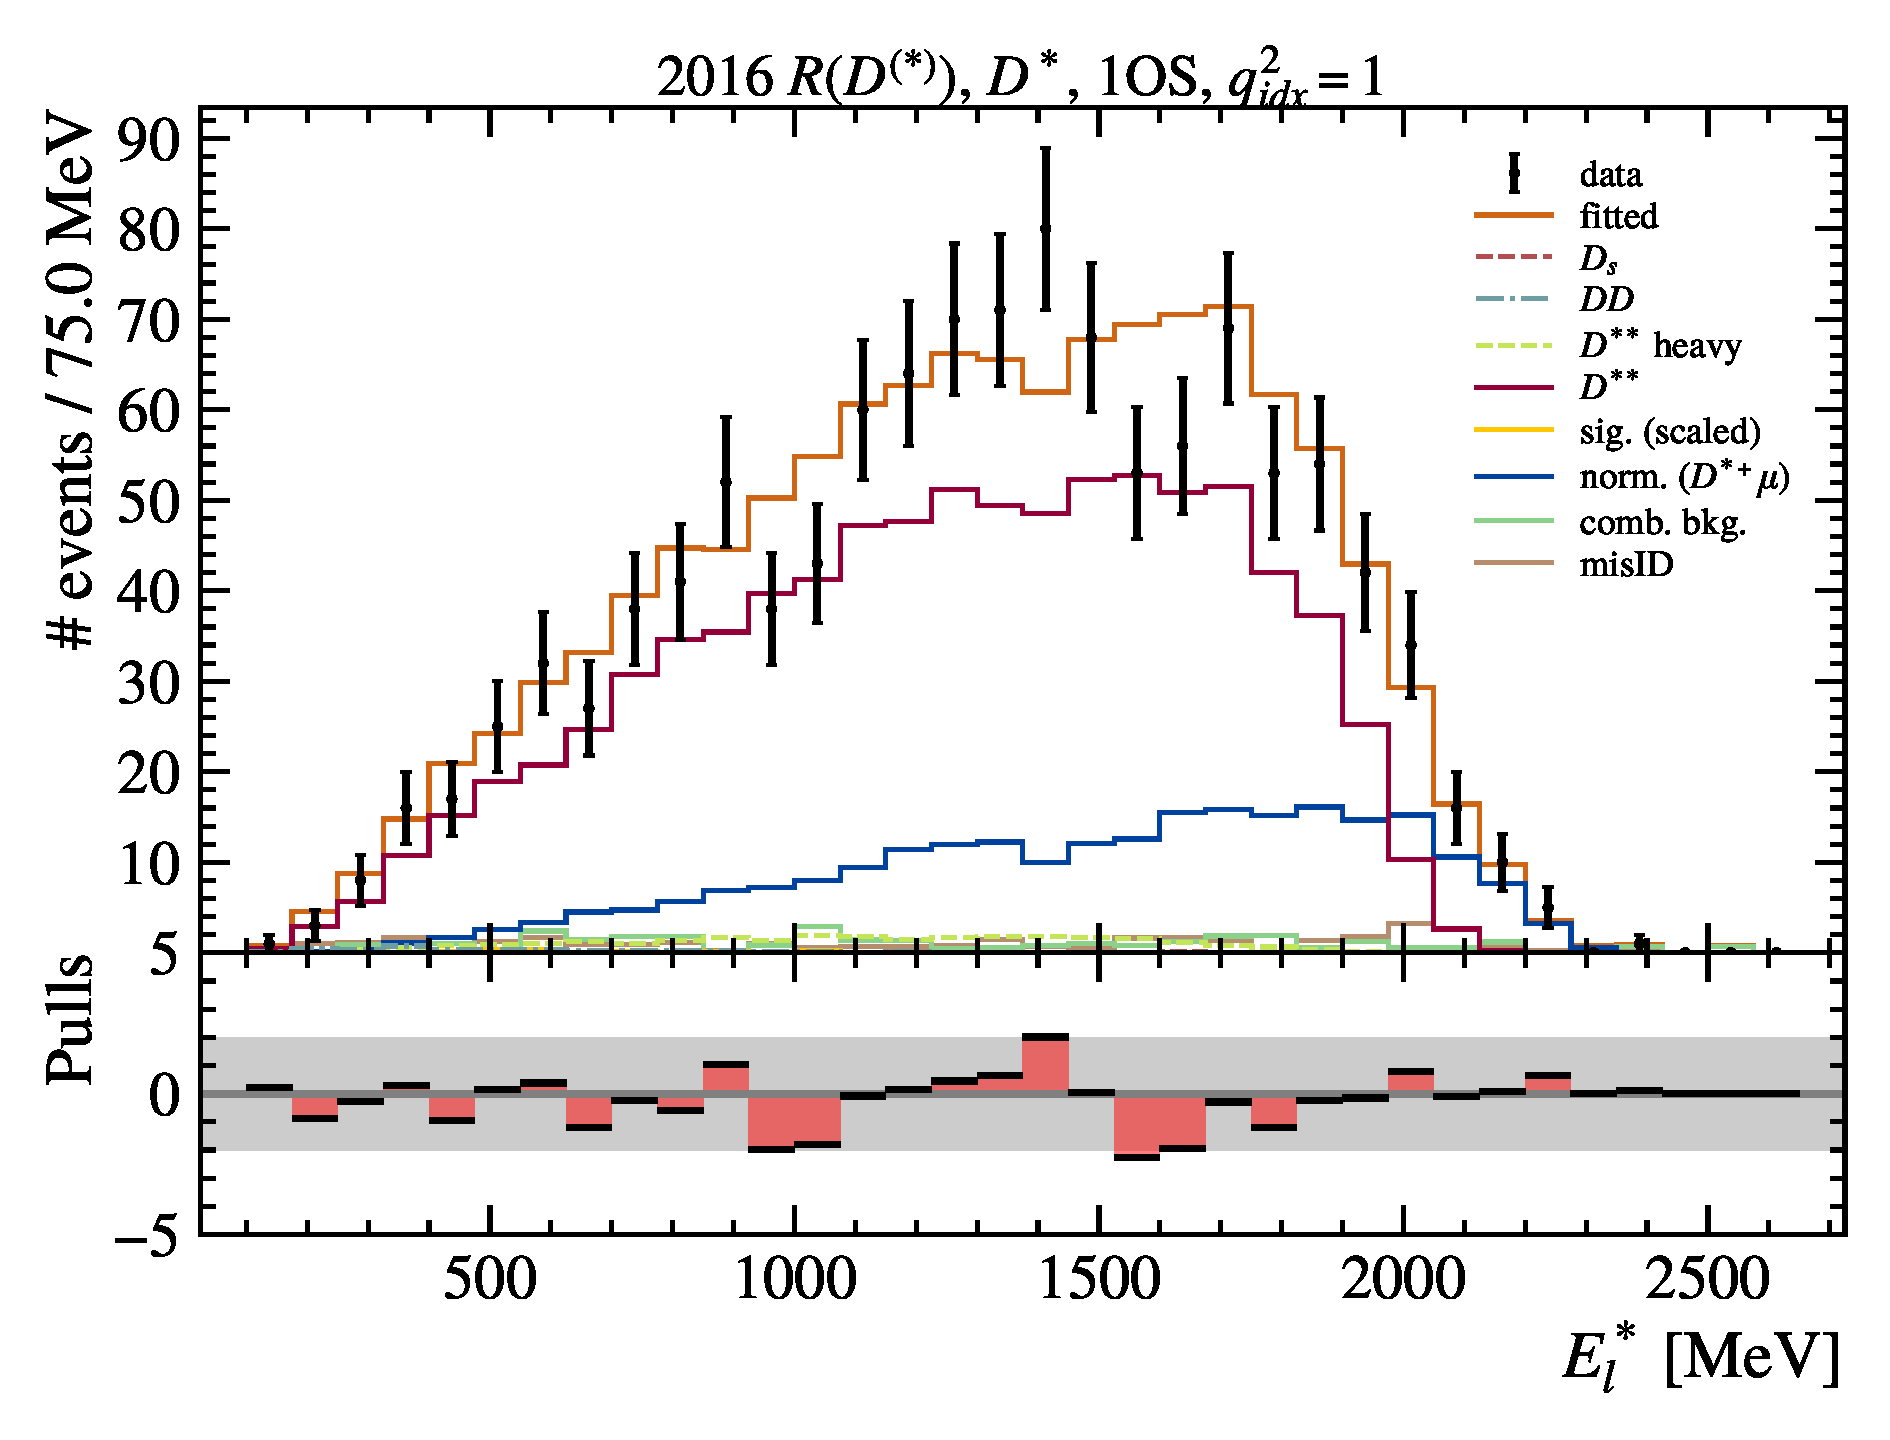
\includegraphics[width=0.24\textwidth]{./figs-fit-fit-results/ctrl-fit/lines_q2_slices/fit_result-lines_q2_idx1-Dst-1os-el.pdf}
    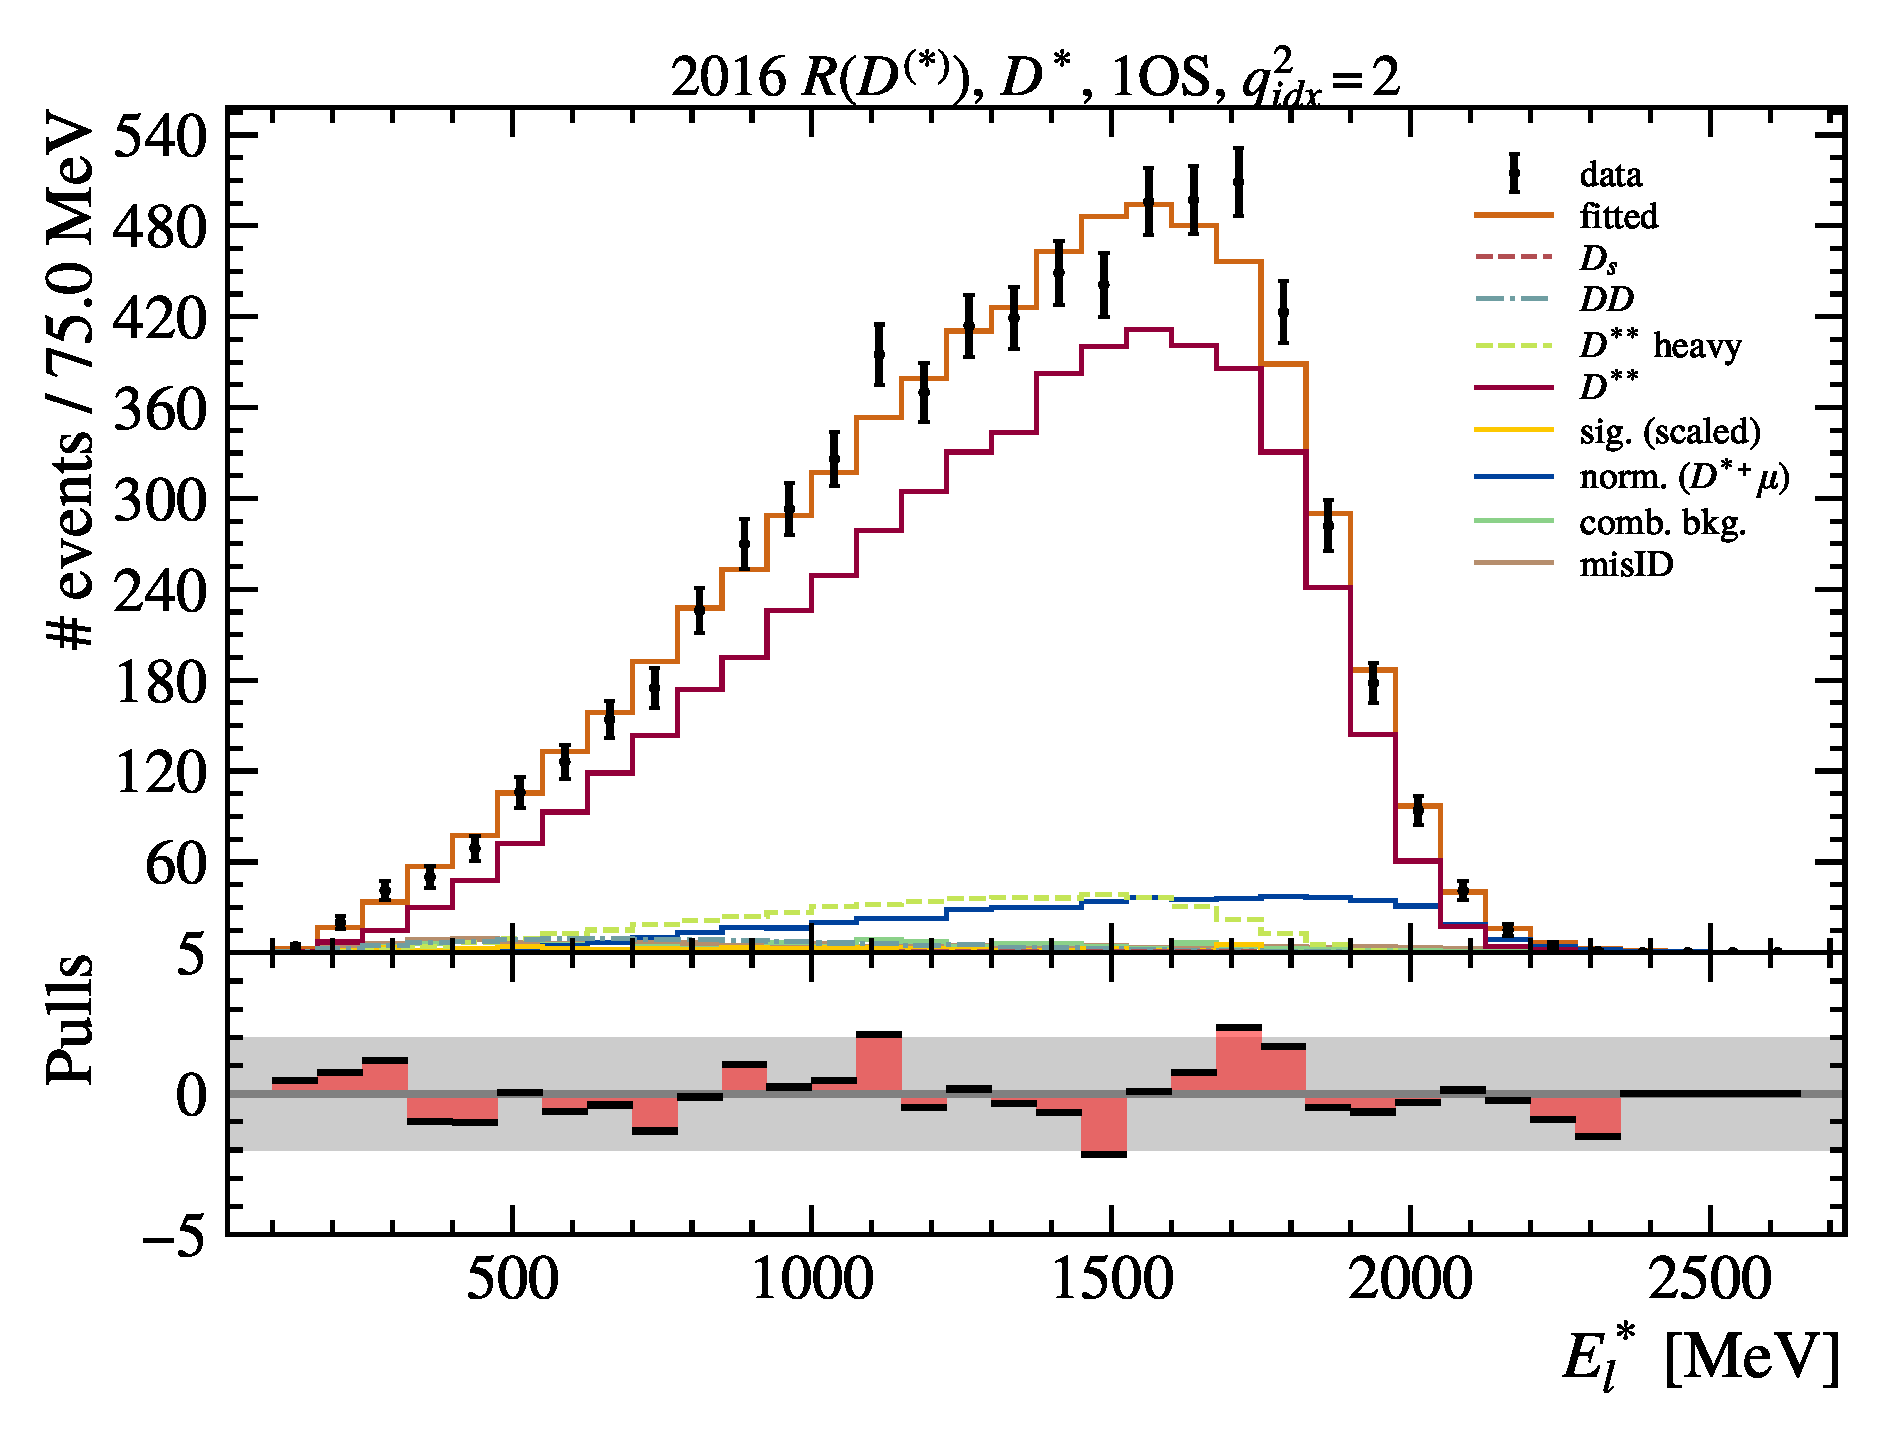
\includegraphics[width=0.24\textwidth]{./figs-fit-fit-results/ctrl-fit/lines_q2_slices/fit_result-lines_q2_idx2-Dst-1os-el.pdf}
    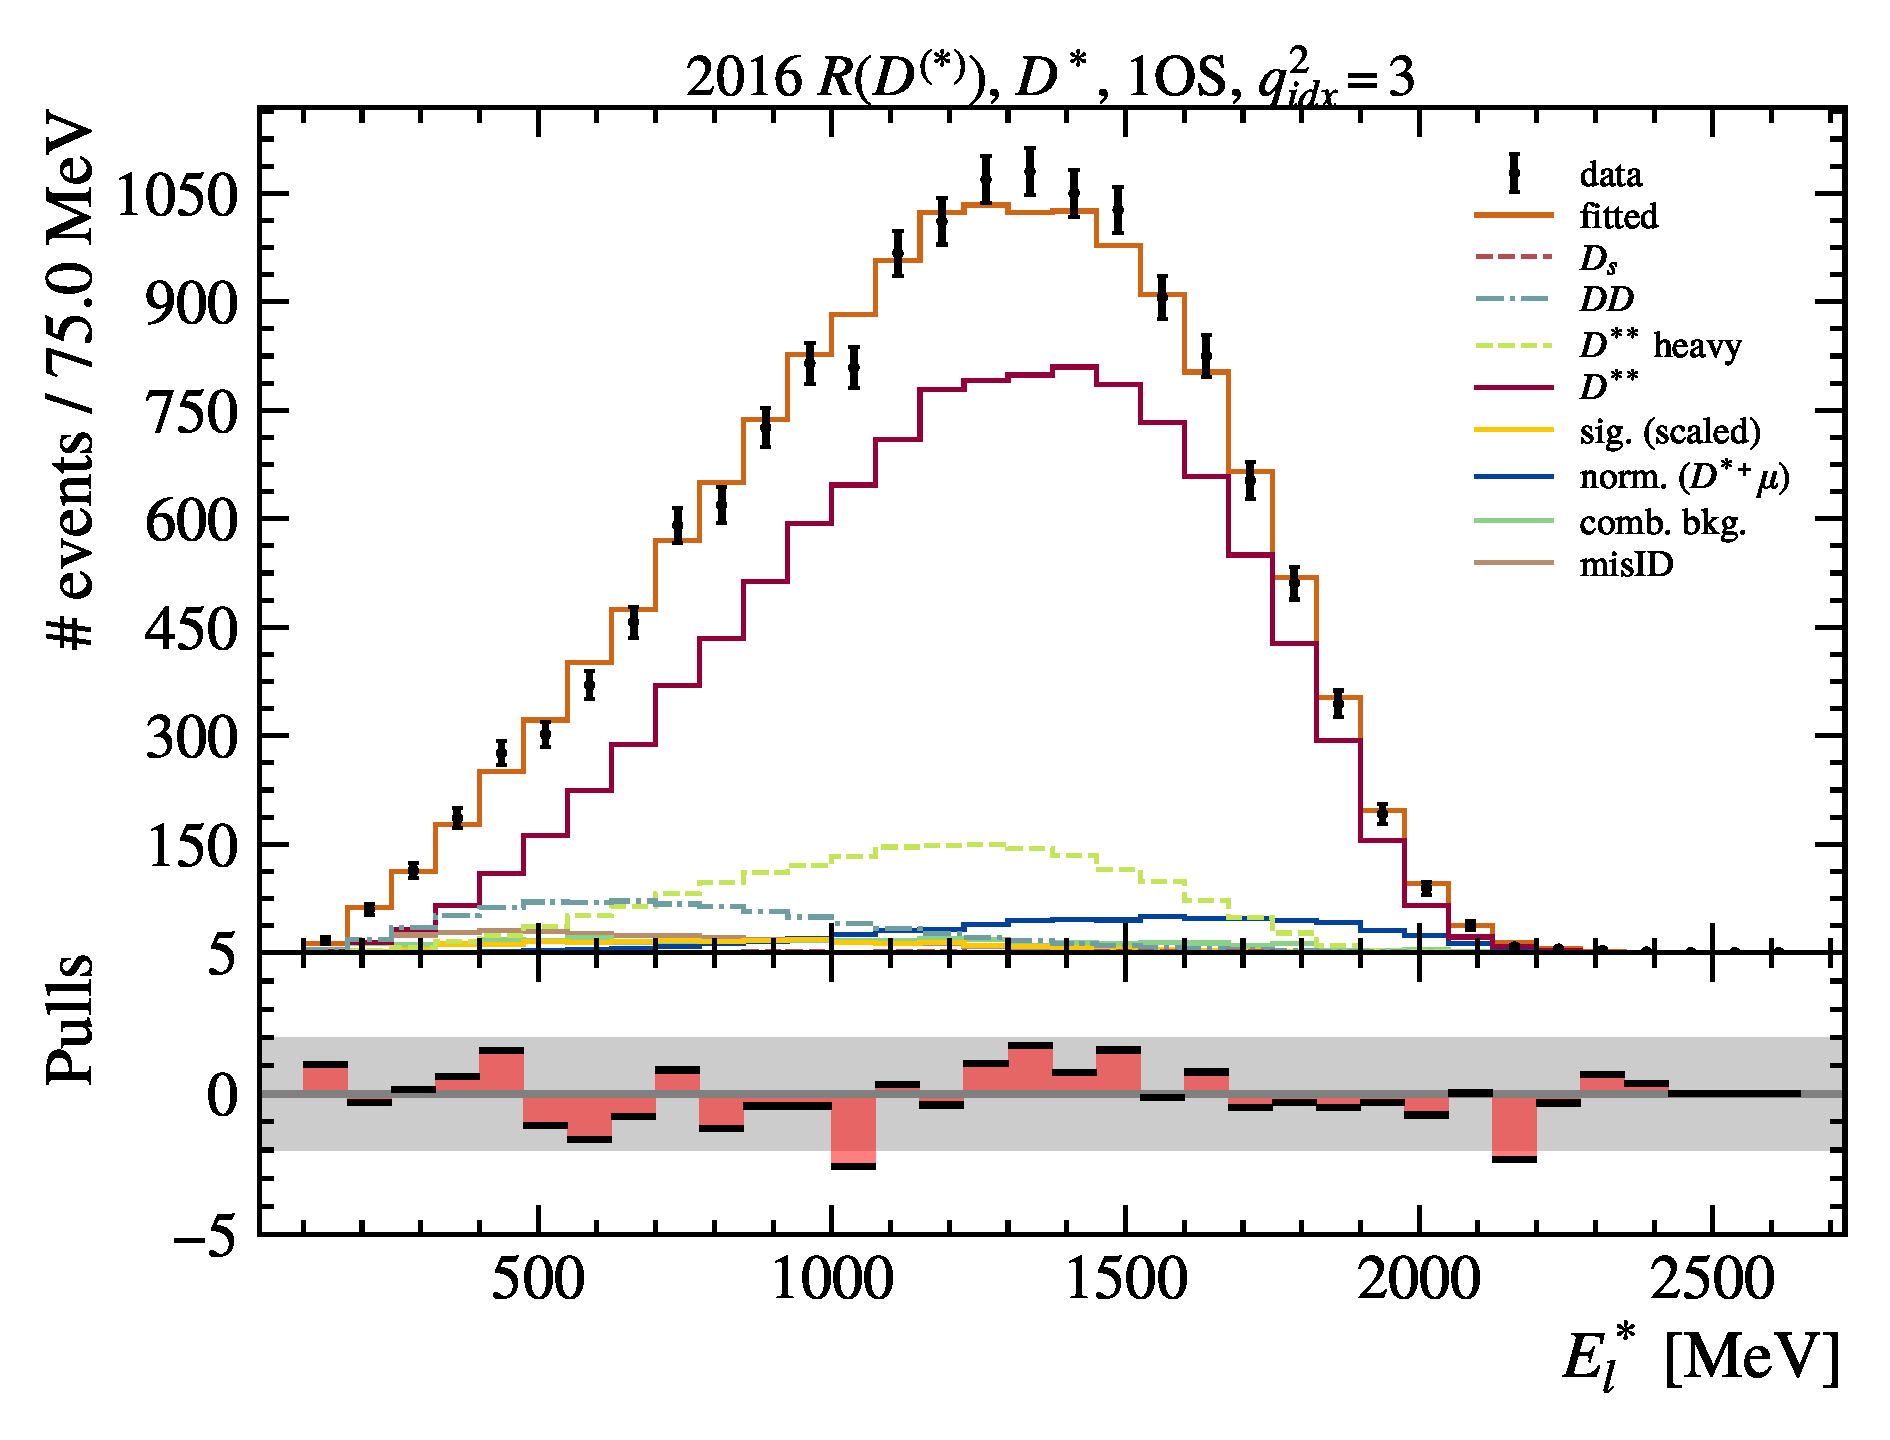
\includegraphics[width=0.24\textwidth]{./figs-fit-fit-results/ctrl-fit/lines_q2_slices/fit_result-lines_q2_idx3-Dst-1os-el.pdf}
    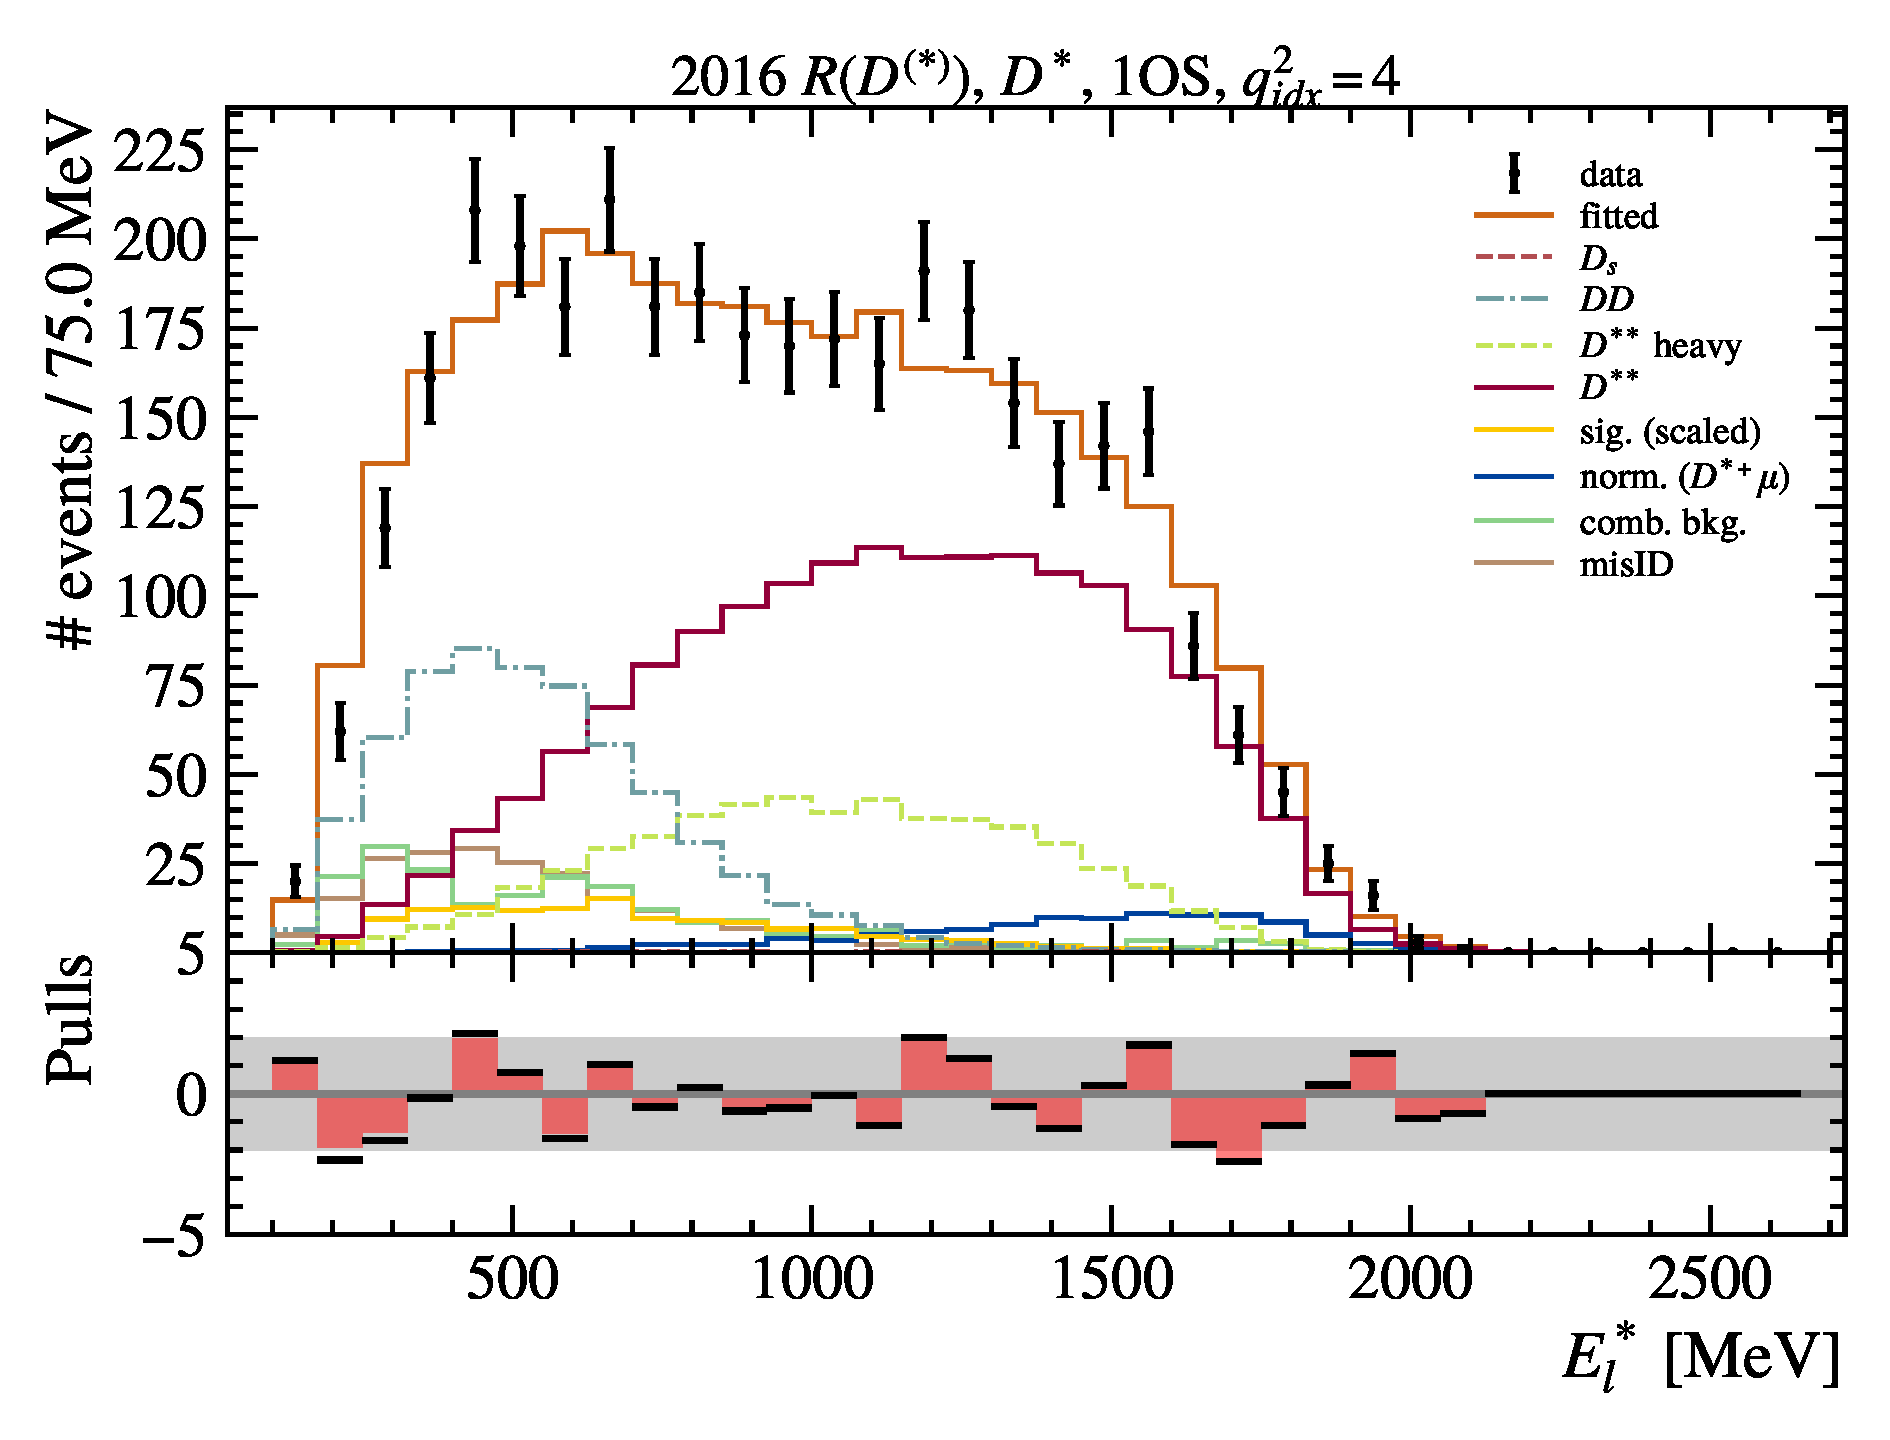
\includegraphics[width=0.24\textwidth]{./figs-fit-fit-results/ctrl-fit/lines_q2_slices/fit_result-lines_q2_idx4-Dst-1os-el.pdf}

    \caption{Control fit for 1OS sample, \Dstar channel.}
    \label{fig:ctrl-1os-dst}
\end{figure}

\begin{figure}[!htb]
    \centering
    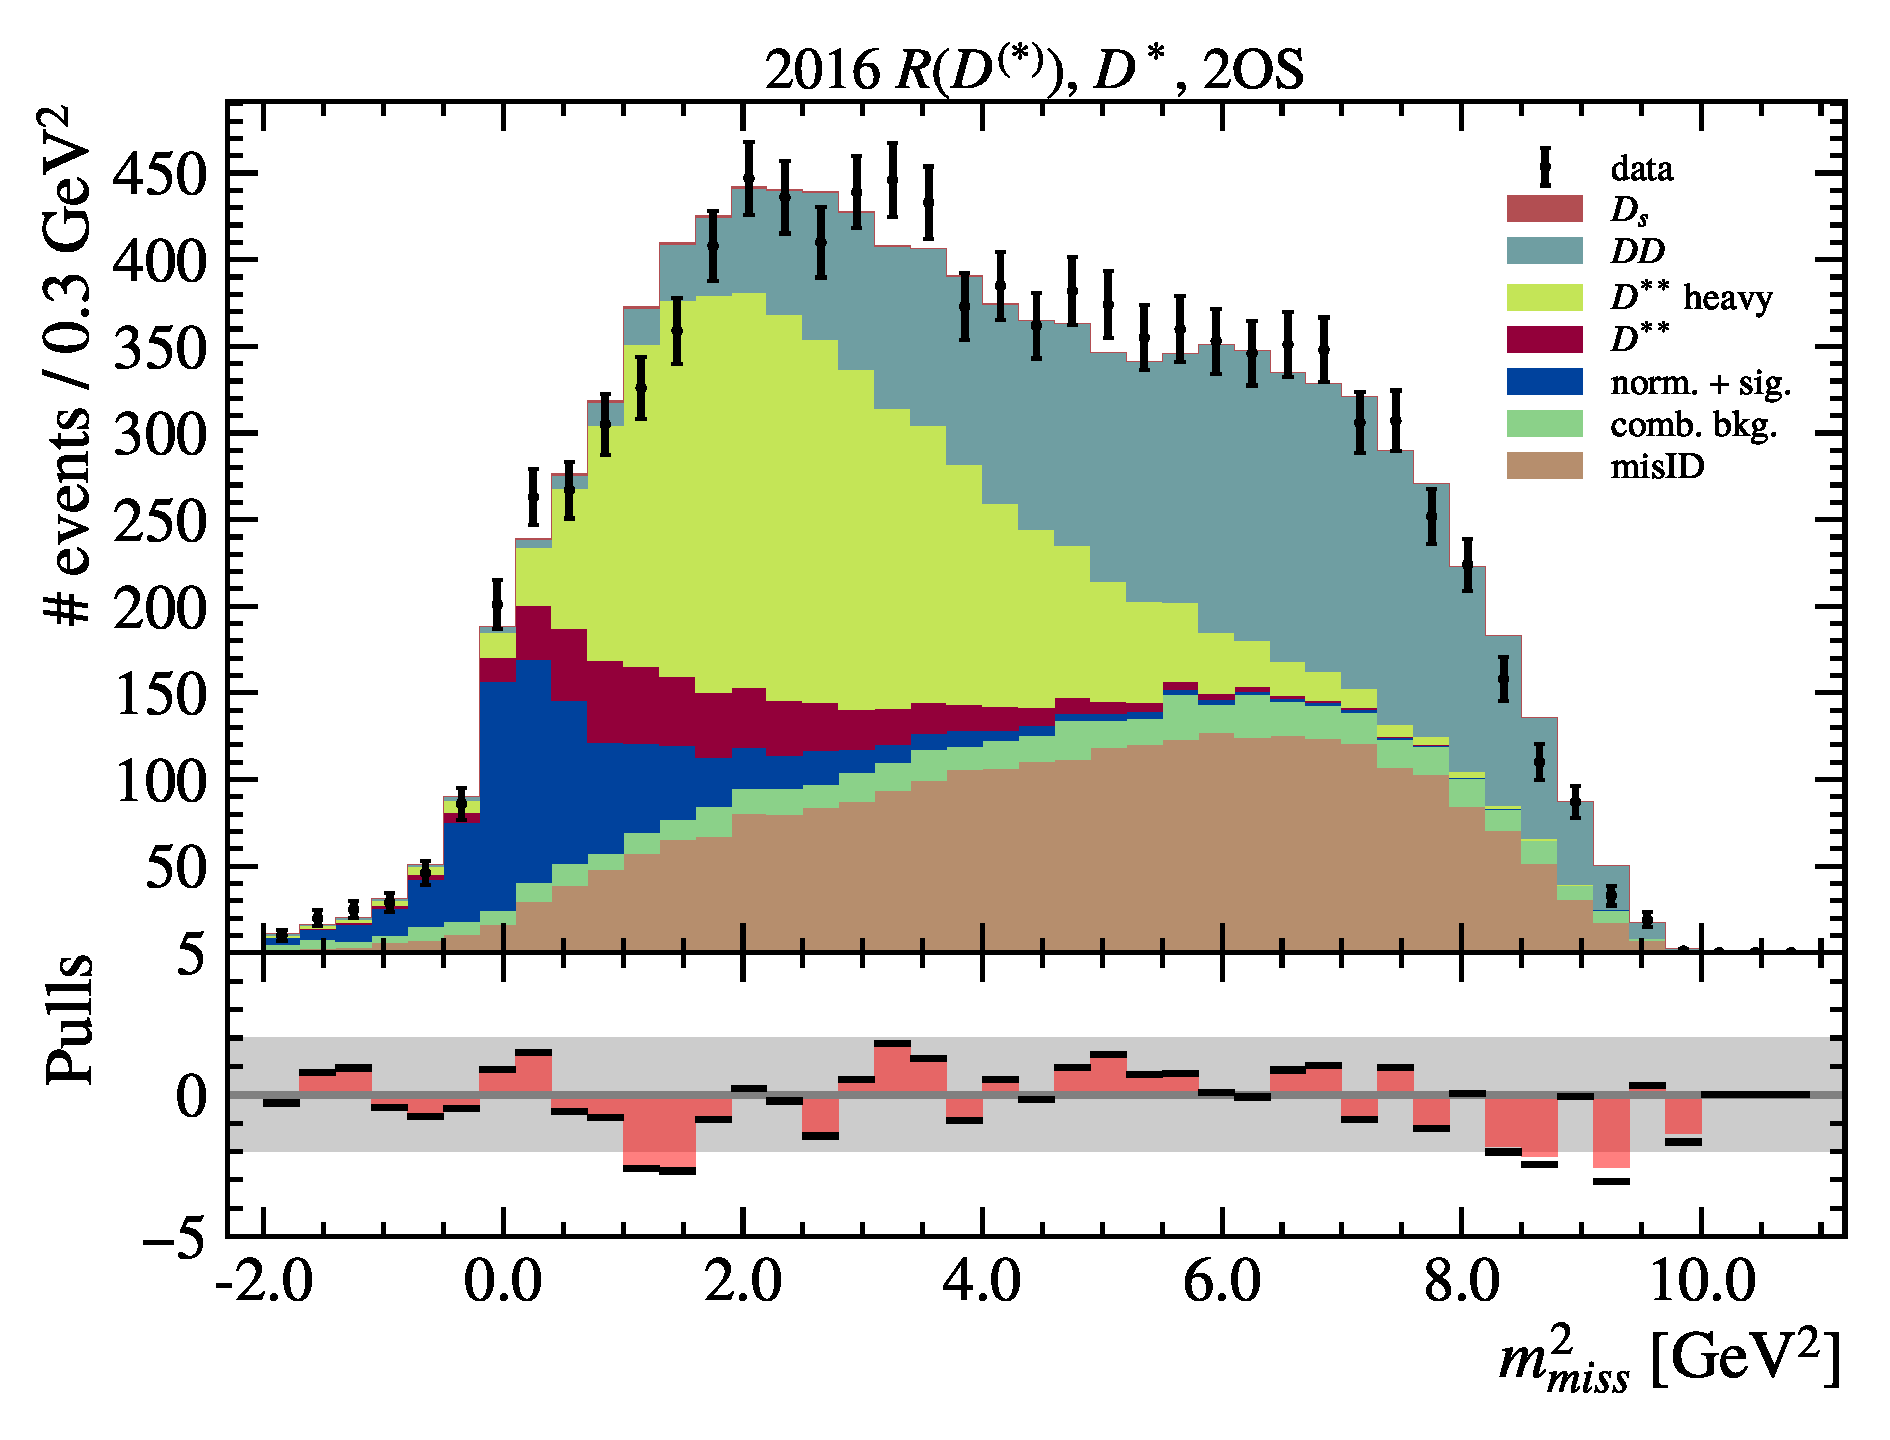
\includegraphics[width=0.32\textwidth]{./figs-fit-fit-results/ctrl-fit/stacked/fit_result-stacked-Dst-2os-mmiss2.pdf}
    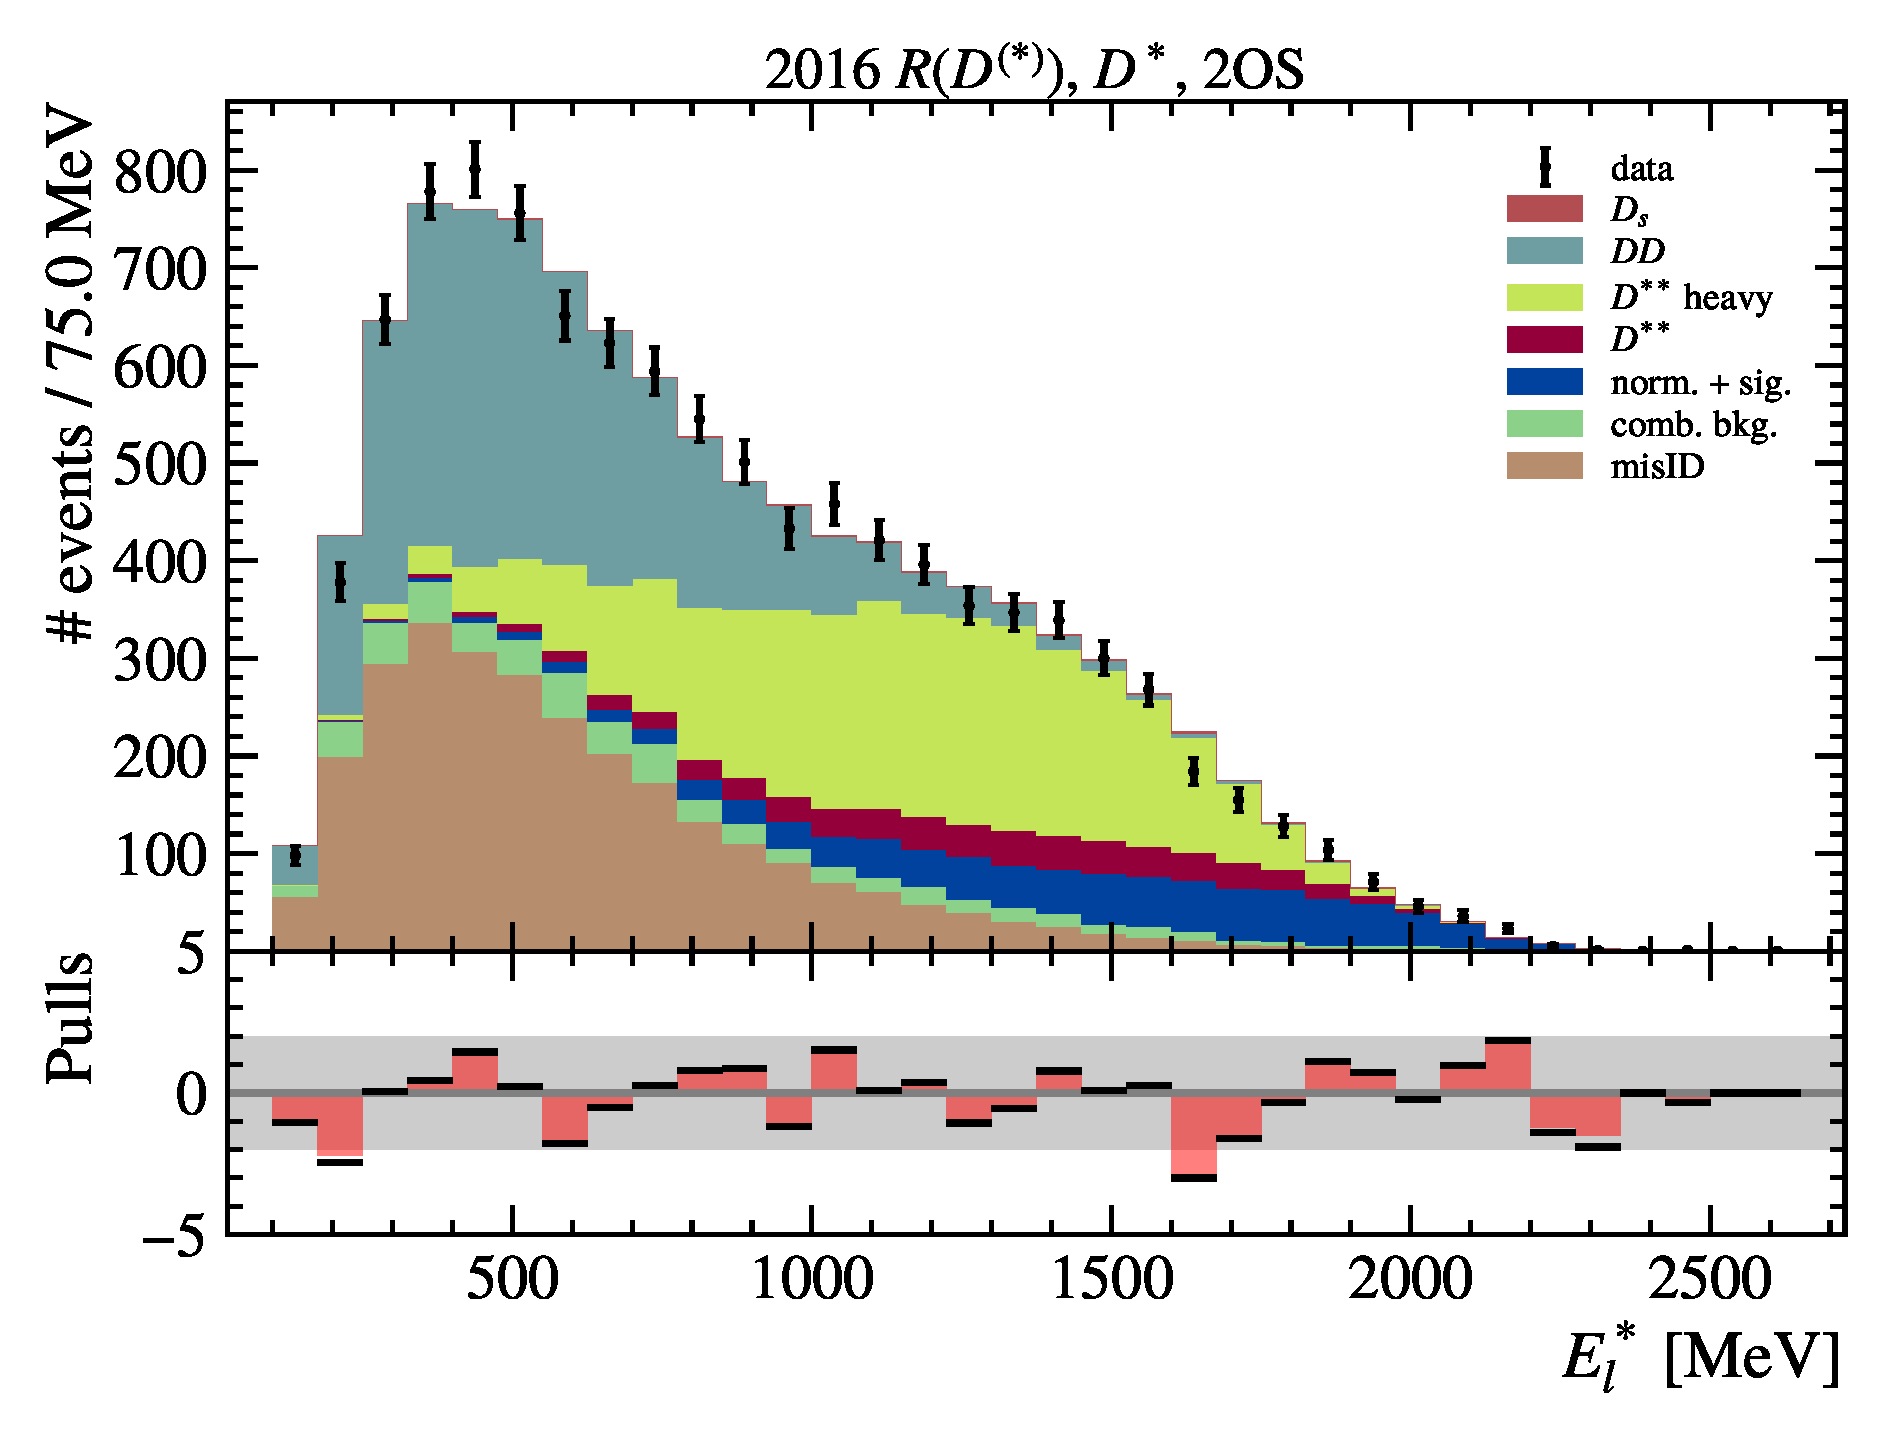
\includegraphics[width=0.32\textwidth]{./figs-fit-fit-results/ctrl-fit/stacked/fit_result-stacked-Dst-2os-el.pdf}
    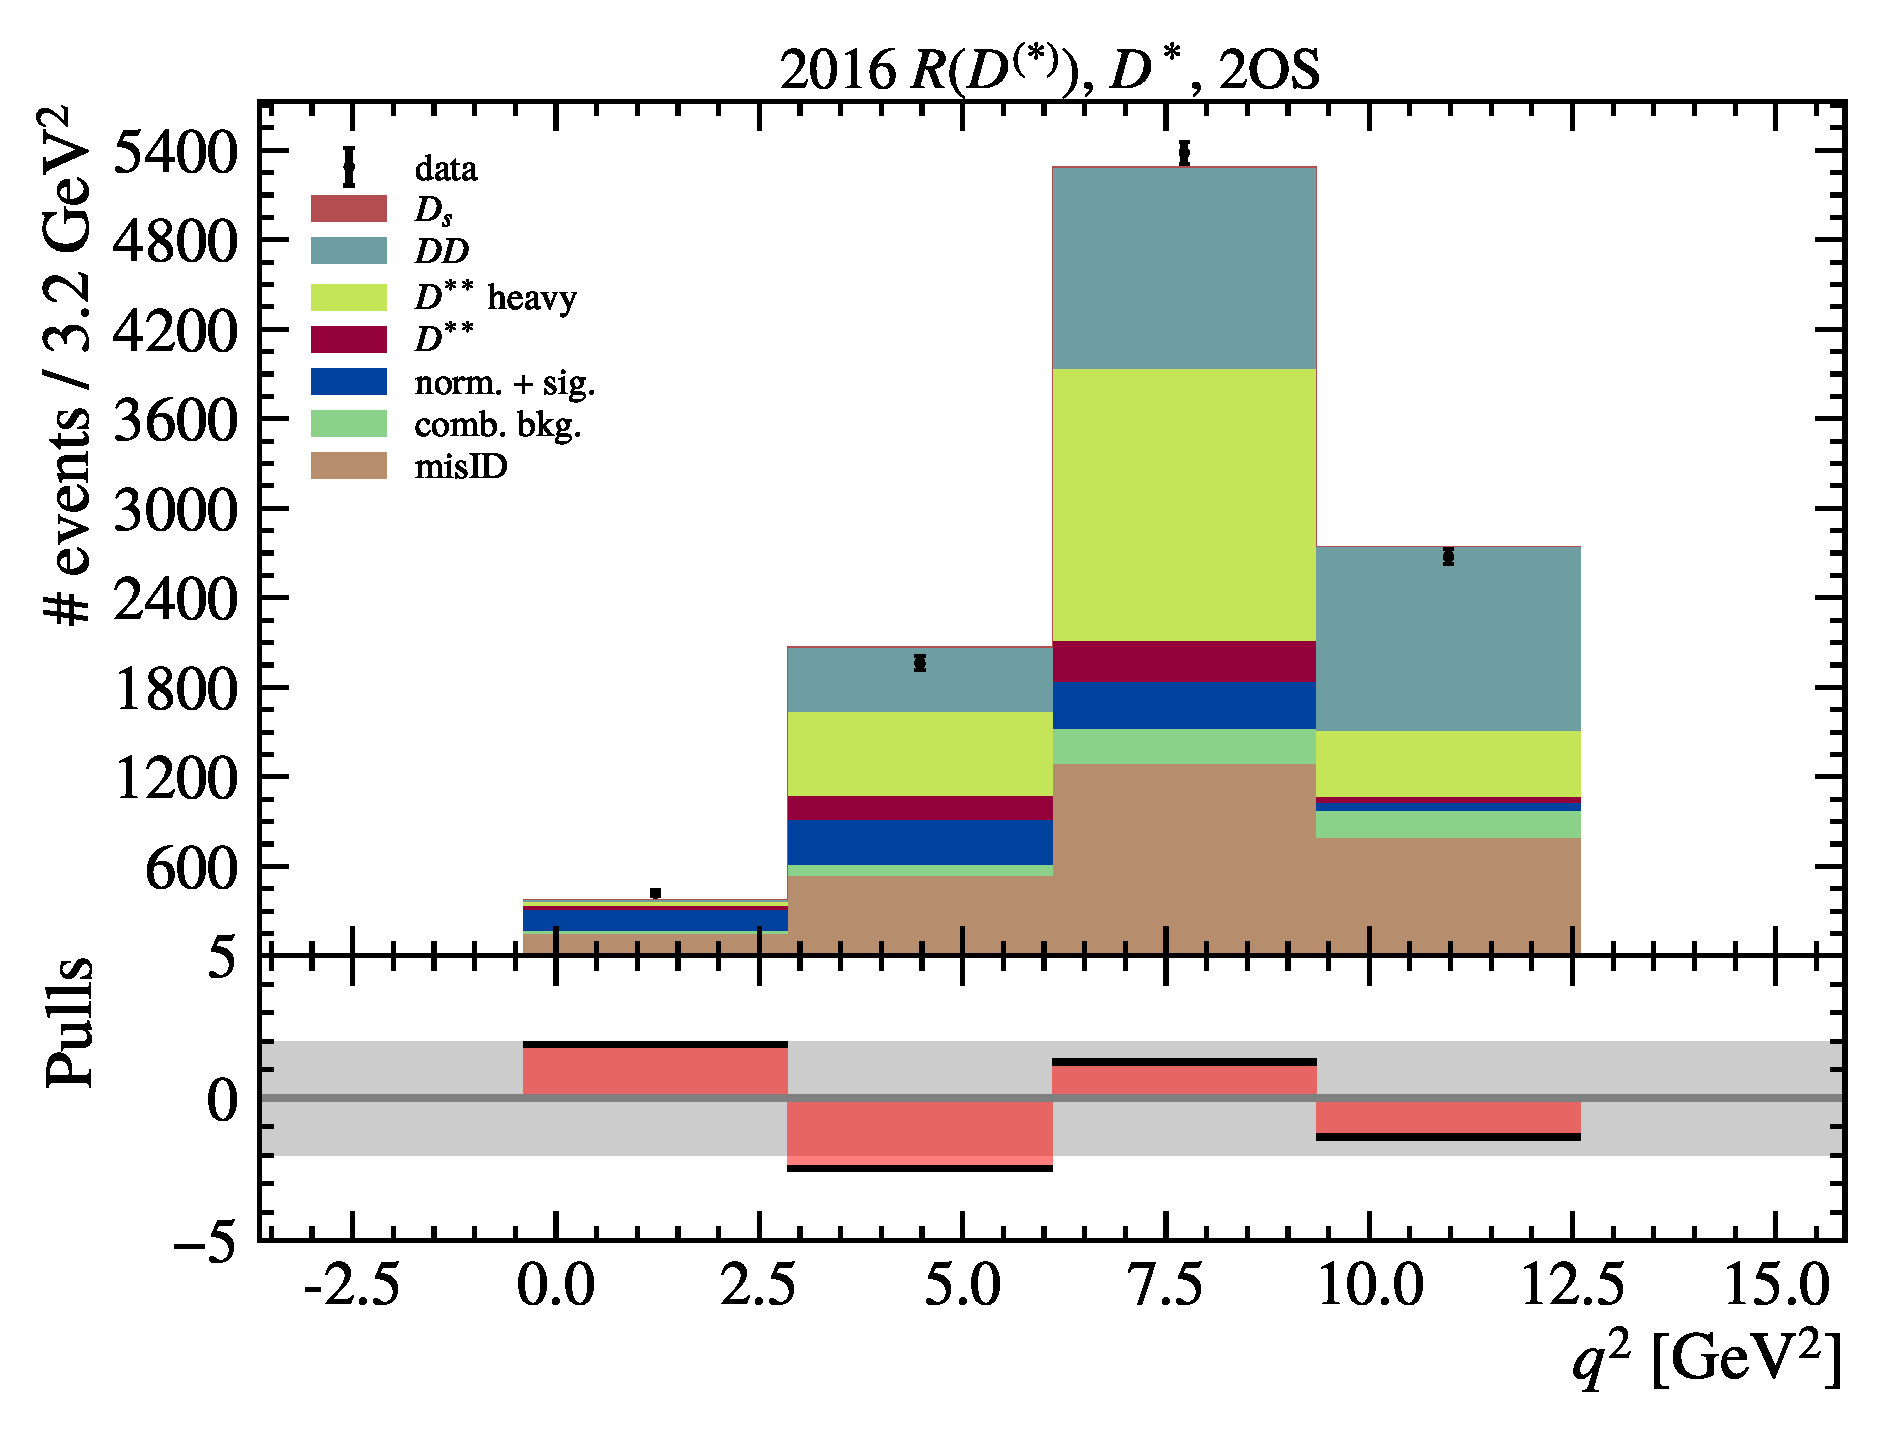
\includegraphics[width=0.32\textwidth]{./figs-fit-fit-results/ctrl-fit/stacked/fit_result-stacked-Dst-2os-q2.pdf}

    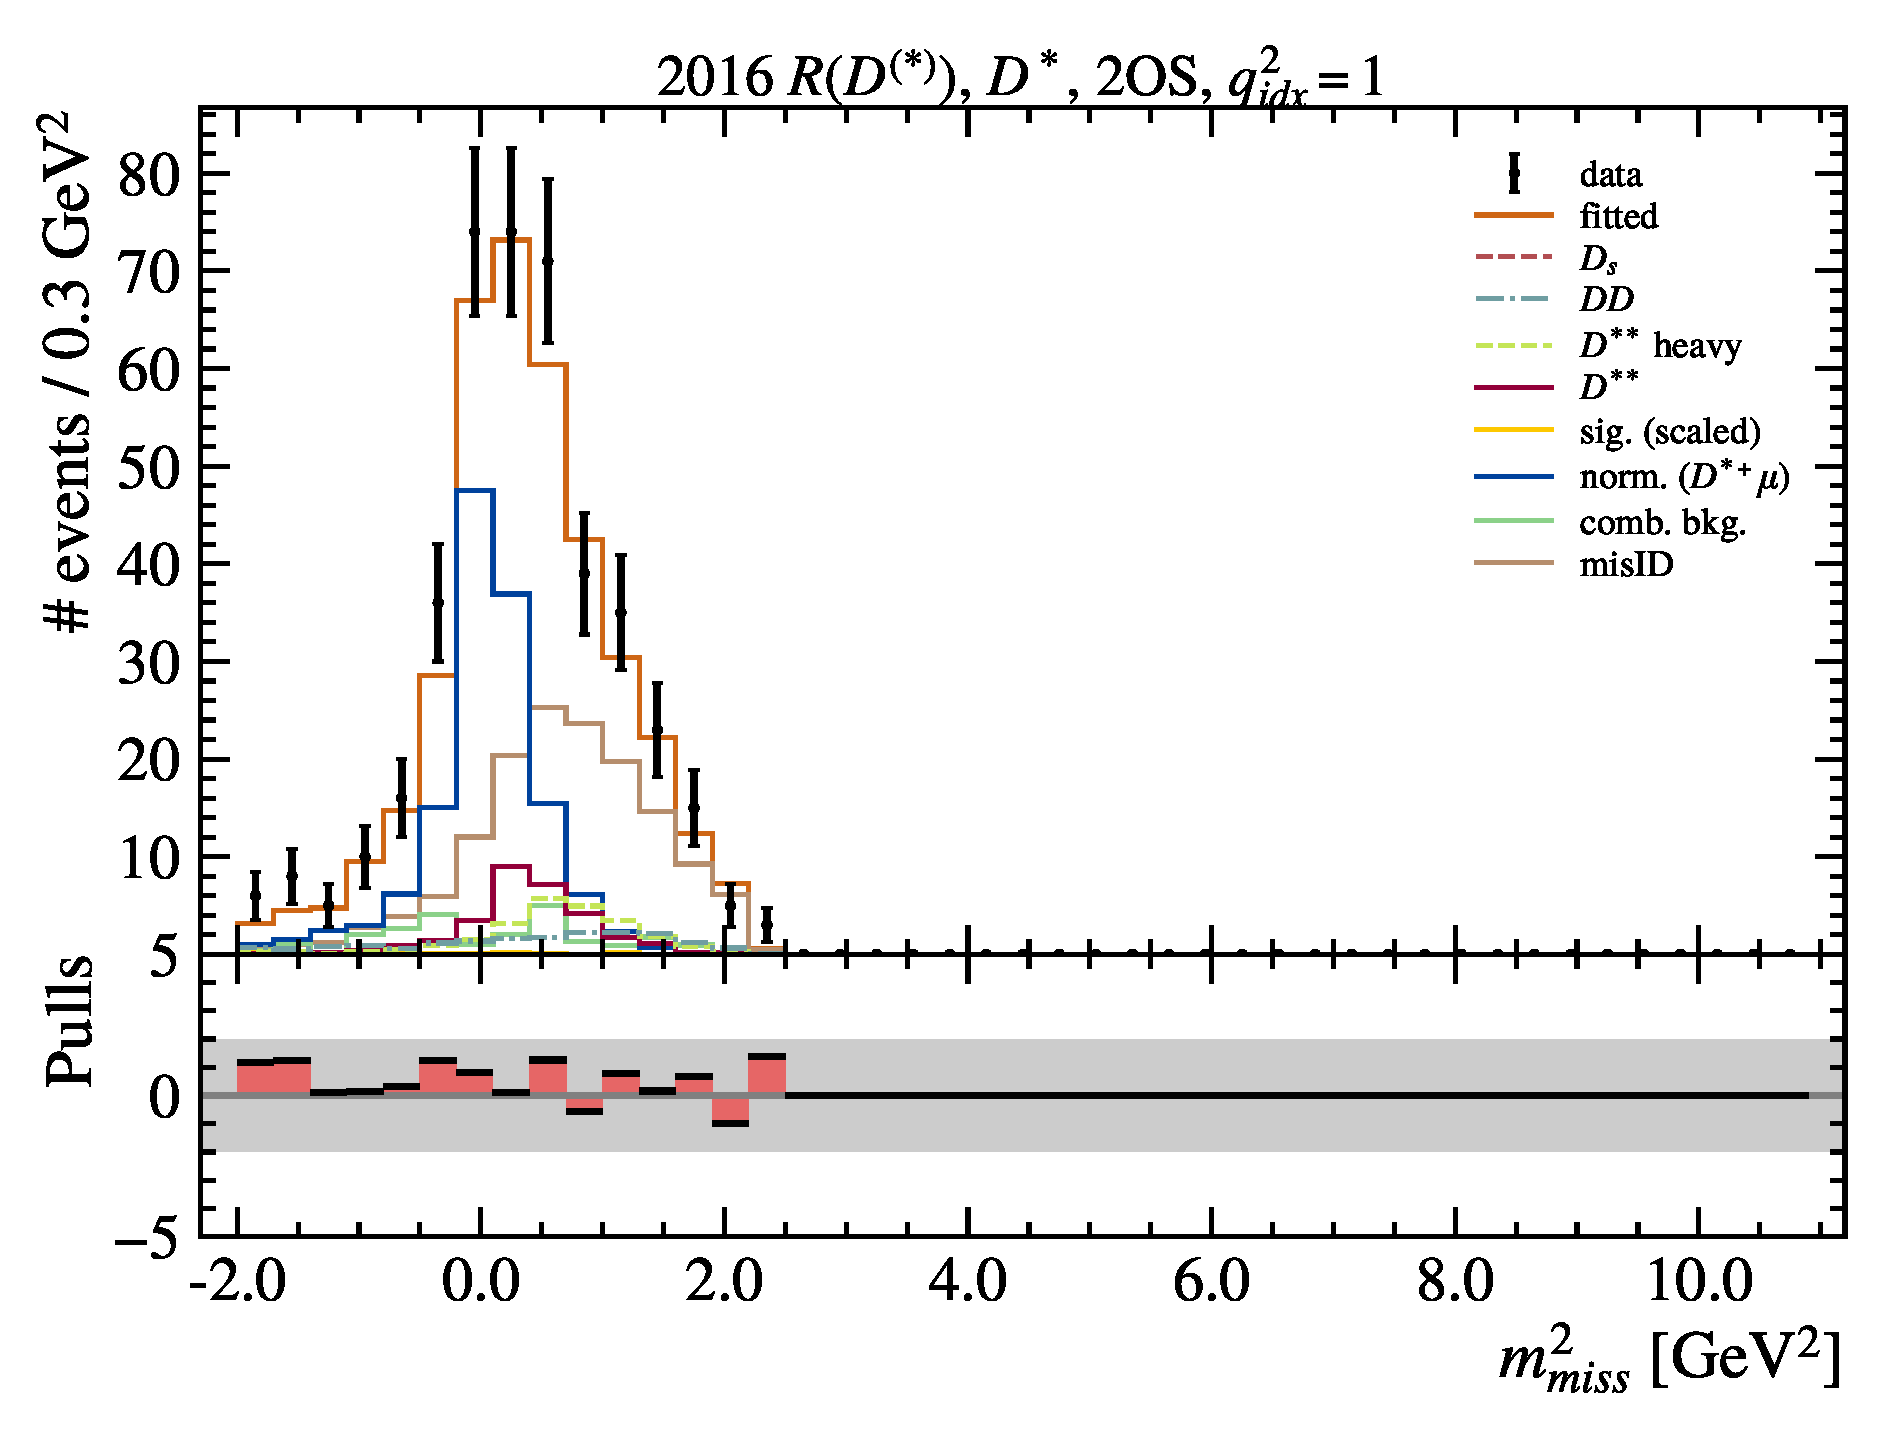
\includegraphics[width=0.24\textwidth]{./figs-fit-fit-results/ctrl-fit/lines_q2_slices/fit_result-lines_q2_idx1-Dst-2os-mmiss2.pdf}
    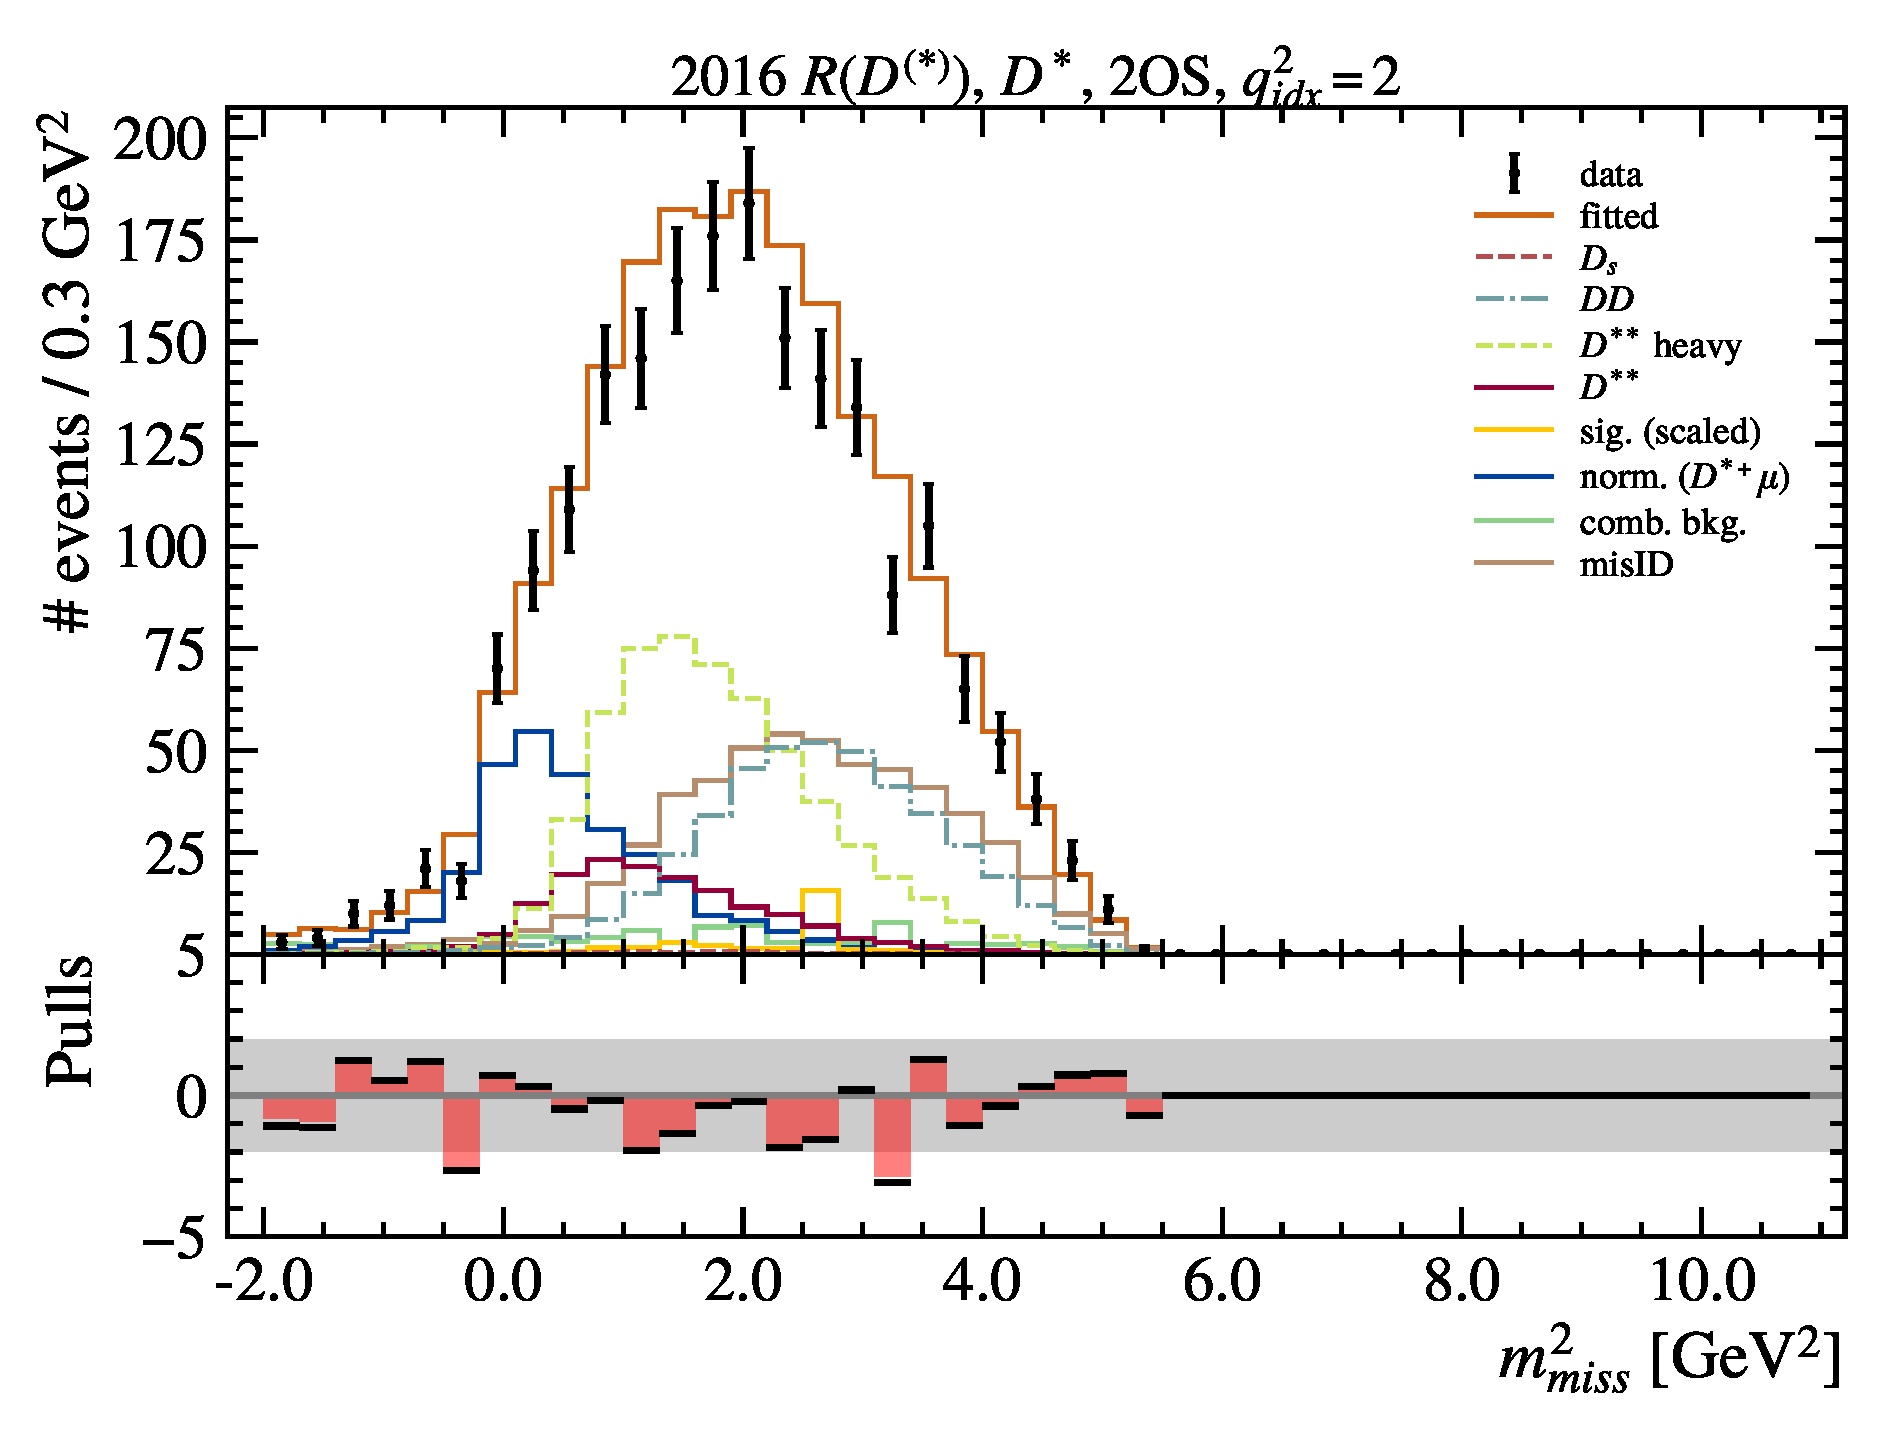
\includegraphics[width=0.24\textwidth]{./figs-fit-fit-results/ctrl-fit/lines_q2_slices/fit_result-lines_q2_idx2-Dst-2os-mmiss2.pdf}
    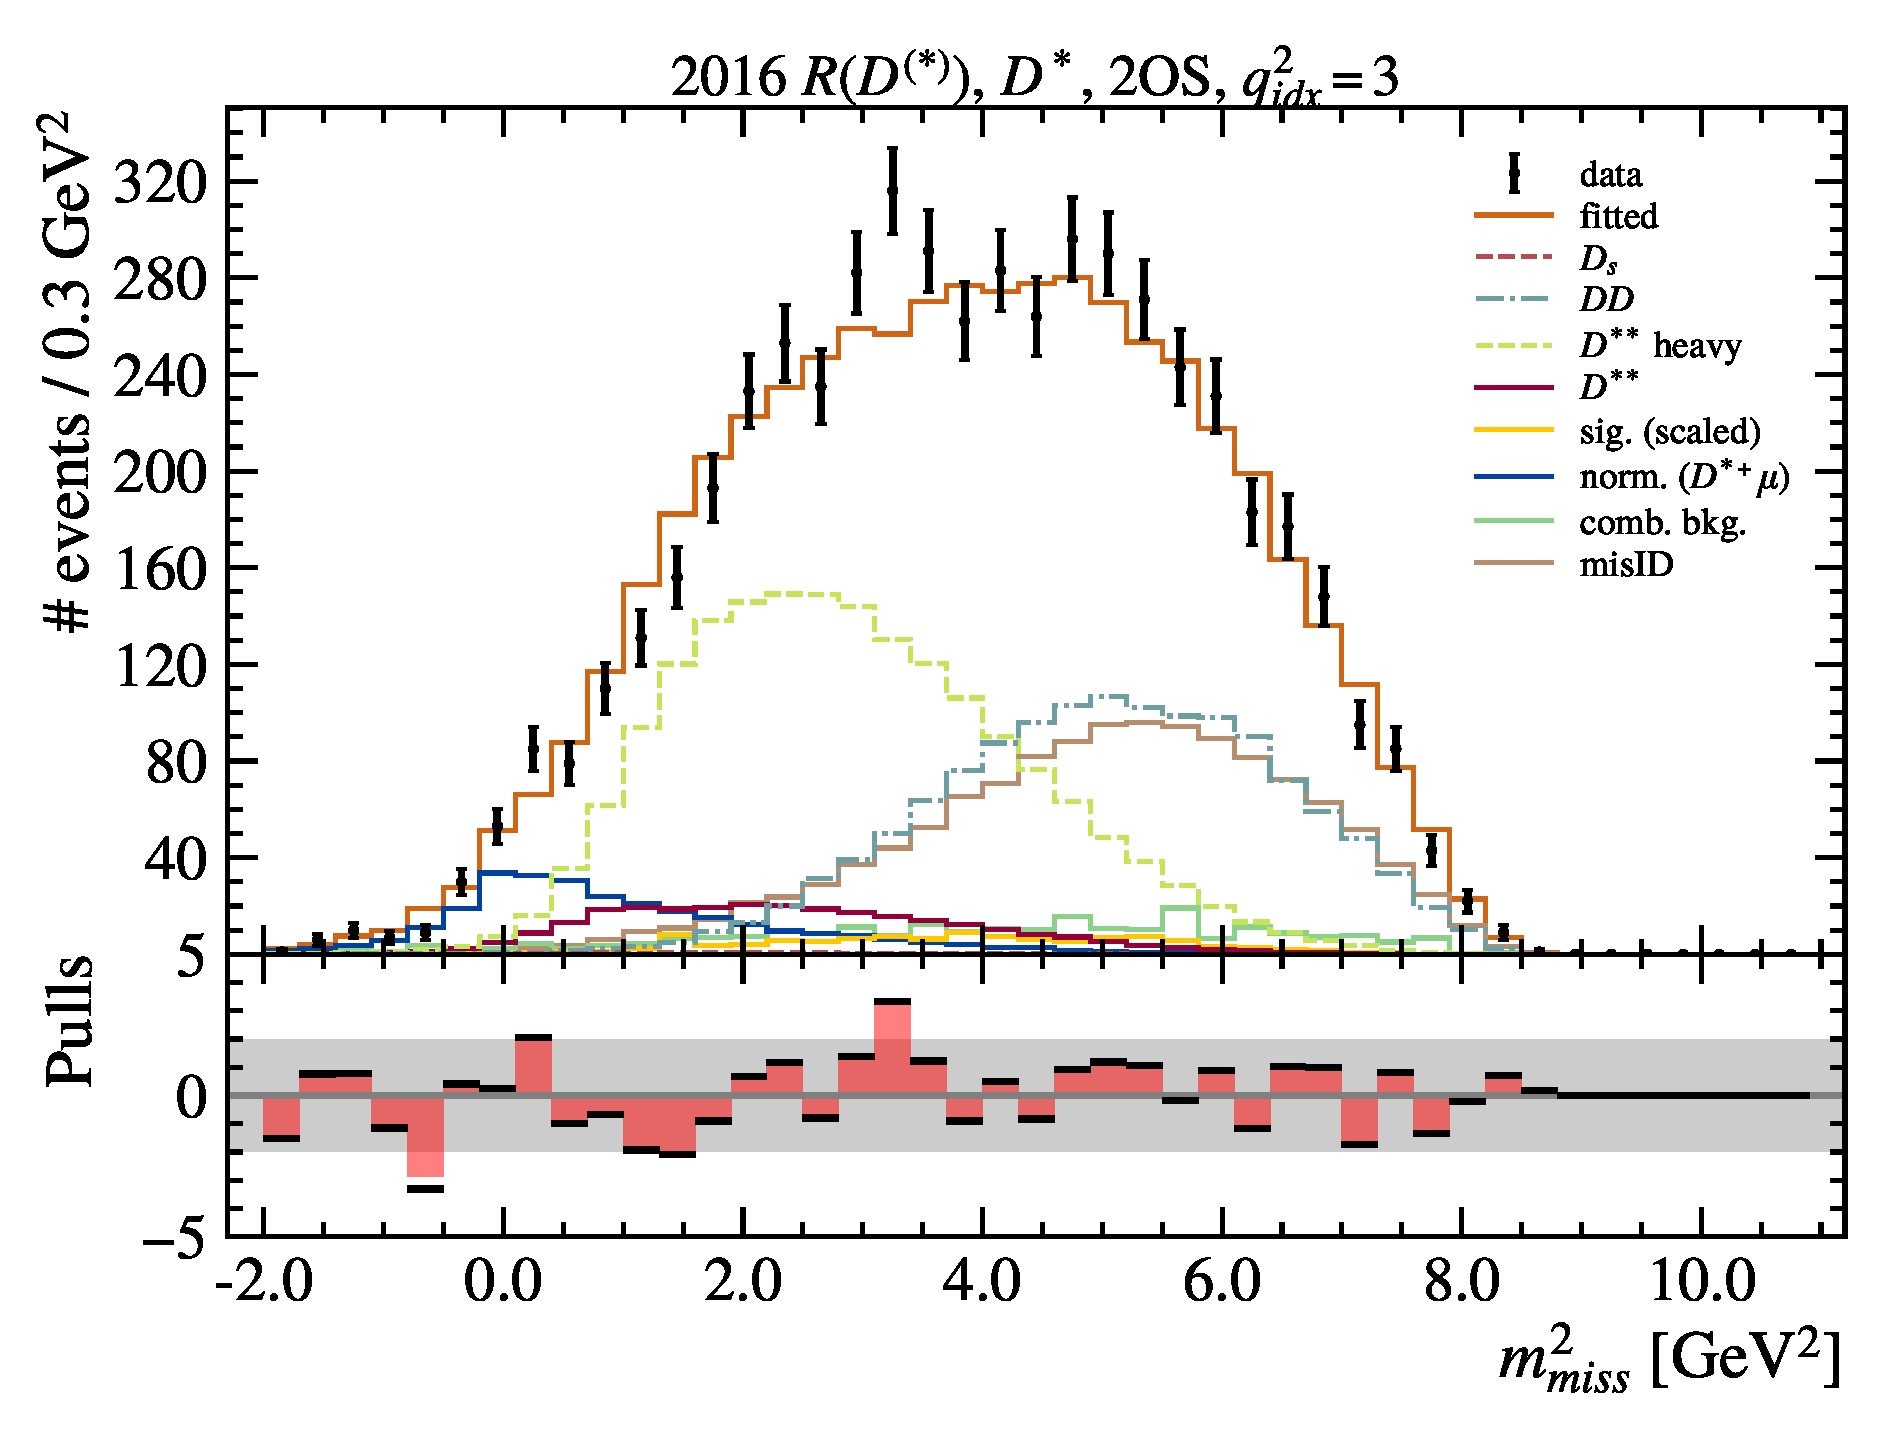
\includegraphics[width=0.24\textwidth]{./figs-fit-fit-results/ctrl-fit/lines_q2_slices/fit_result-lines_q2_idx3-Dst-2os-mmiss2.pdf}
    \includegraphics[width=0.24\textwidth]{./figs-fit-fit-results/ctrl-fit/lines_q2_slices/fit_result-lines_q2_idx4-Dst-2os-mmiss2.pdf}

    \includegraphics[width=0.24\textwidth]{./figs-fit-fit-results/ctrl-fit/lines_q2_slices/fit_result-lines_q2_idx1-Dst-2os-el.pdf}
    \includegraphics[width=0.24\textwidth]{./figs-fit-fit-results/ctrl-fit/lines_q2_slices/fit_result-lines_q2_idx2-Dst-2os-el.pdf}
    \includegraphics[width=0.24\textwidth]{./figs-fit-fit-results/ctrl-fit/lines_q2_slices/fit_result-lines_q2_idx3-Dst-2os-el.pdf}
    \includegraphics[width=0.24\textwidth]{./figs-fit-fit-results/ctrl-fit/lines_q2_slices/fit_result-lines_q2_idx4-Dst-2os-el.pdf}

    \caption{Control fit for 2OS sample, \Dstar channel.}
    \label{fig:ctrl-2os-dst}
\end{figure}

\begin{figure}[!htb]
    \centering
    \includegraphics[width=0.32\textwidth]{./figs-fit-fit-results/ctrl-fit/stacked/fit_result-stacked-Dst-dd-mmiss2.pdf}
    \includegraphics[width=0.32\textwidth]{./figs-fit-fit-results/ctrl-fit/stacked/fit_result-stacked-Dst-dd-el.pdf}
    \includegraphics[width=0.32\textwidth]{./figs-fit-fit-results/ctrl-fit/stacked/fit_result-stacked-Dst-dd-q2.pdf}

    \includegraphics[width=0.24\textwidth]{./figs-fit-fit-results/ctrl-fit/lines_q2_slices/fit_result-lines_q2_idx1-Dst-dd-mmiss2.pdf}
    \includegraphics[width=0.24\textwidth]{./figs-fit-fit-results/ctrl-fit/lines_q2_slices/fit_result-lines_q2_idx2-Dst-dd-mmiss2.pdf}
    \includegraphics[width=0.24\textwidth]{./figs-fit-fit-results/ctrl-fit/lines_q2_slices/fit_result-lines_q2_idx3-Dst-dd-mmiss2.pdf}
    \includegraphics[width=0.24\textwidth]{./figs-fit-fit-results/ctrl-fit/lines_q2_slices/fit_result-lines_q2_idx4-Dst-dd-mmiss2.pdf}

    \includegraphics[width=0.24\textwidth]{./figs-fit-fit-results/ctrl-fit/lines_q2_slices/fit_result-lines_q2_idx1-Dst-dd-el.pdf}
    \includegraphics[width=0.24\textwidth]{./figs-fit-fit-results/ctrl-fit/lines_q2_slices/fit_result-lines_q2_idx2-Dst-dd-el.pdf}
    \includegraphics[width=0.24\textwidth]{./figs-fit-fit-results/ctrl-fit/lines_q2_slices/fit_result-lines_q2_idx3-Dst-dd-el.pdf}
    \includegraphics[width=0.24\textwidth]{./figs-fit-fit-results/ctrl-fit/lines_q2_slices/fit_result-lines_q2_idx4-Dst-dd-el.pdf}

    \caption{Control fit for DD sample, \Dstar channel.}
    \label{fig:ctrl-dd-dst}
\end{figure}


% sig
\begin{figure}[!htb]
    \centering
    \includegraphics[width=0.32\textwidth]{./figs-fit-fit-results/sig-fit/stacked/fit_result-stacked-D0-iso-mmiss2.pdf}
    \includegraphics[width=0.32\textwidth]{./figs-fit-fit-results/sig-fit/stacked/fit_result-stacked-D0-iso-el.pdf}
    \includegraphics[width=0.32\textwidth]{./figs-fit-fit-results/sig-fit/stacked/fit_result-stacked-D0-iso-q2.pdf}

    \includegraphics[width=0.24\textwidth]{./figs-fit-fit-results/sig-fit/lines_q2_slices/fit_result-lines_q2_idx1-D0-iso-mmiss2.pdf}
    \includegraphics[width=0.24\textwidth]{./figs-fit-fit-results/sig-fit/lines_q2_slices/fit_result-lines_q2_idx2-D0-iso-mmiss2.pdf}
    \includegraphics[width=0.24\textwidth]{./figs-fit-fit-results/sig-fit/lines_q2_slices/fit_result-lines_q2_idx3-D0-iso-mmiss2.pdf}
    \includegraphics[width=0.24\textwidth]{./figs-fit-fit-results/sig-fit/lines_q2_slices/fit_result-lines_q2_idx4-D0-iso-mmiss2.pdf}

    \includegraphics[width=0.24\textwidth]{./figs-fit-fit-results/sig-fit/lines_q2_slices/fit_result-lines_q2_idx1-D0-iso-el.pdf}
    \includegraphics[width=0.24\textwidth]{./figs-fit-fit-results/sig-fit/lines_q2_slices/fit_result-lines_q2_idx2-D0-iso-el.pdf}
    \includegraphics[width=0.24\textwidth]{./figs-fit-fit-results/sig-fit/lines_q2_slices/fit_result-lines_q2_idx3-D0-iso-el.pdf}
    \includegraphics[width=0.24\textwidth]{./figs-fit-fit-results/sig-fit/lines_q2_slices/fit_result-lines_q2_idx4-D0-iso-el.pdf}

    \caption{Signal fit for ISO sample, \Dz channel.}
    \label{fig:sig-d0}
\end{figure}

\begin{figure}[!htb]
    \centering
    \includegraphics[width=0.32\textwidth]{./figs-fit-fit-results/sig-fit/stacked/fit_result-stacked-Dst-iso-mmiss2.pdf}
    \includegraphics[width=0.32\textwidth]{./figs-fit-fit-results/sig-fit/stacked/fit_result-stacked-Dst-iso-el.pdf}
    \includegraphics[width=0.32\textwidth]{./figs-fit-fit-results/sig-fit/stacked/fit_result-stacked-Dst-iso-q2.pdf}

    \includegraphics[width=0.24\textwidth]{./figs-fit-fit-results/sig-fit/lines_q2_slices/fit_result-lines_q2_idx1-Dst-iso-mmiss2.pdf}
    \includegraphics[width=0.24\textwidth]{./figs-fit-fit-results/sig-fit/lines_q2_slices/fit_result-lines_q2_idx2-Dst-iso-mmiss2.pdf}
    \includegraphics[width=0.24\textwidth]{./figs-fit-fit-results/sig-fit/lines_q2_slices/fit_result-lines_q2_idx3-Dst-iso-mmiss2.pdf}
    \includegraphics[width=0.24\textwidth]{./figs-fit-fit-results/sig-fit/lines_q2_slices/fit_result-lines_q2_idx4-Dst-iso-mmiss2.pdf}

    \includegraphics[width=0.24\textwidth]{./figs-fit-fit-results/sig-fit/lines_q2_slices/fit_result-lines_q2_idx1-Dst-iso-el.pdf}
    \includegraphics[width=0.24\textwidth]{./figs-fit-fit-results/sig-fit/lines_q2_slices/fit_result-lines_q2_idx2-Dst-iso-el.pdf}
    \includegraphics[width=0.24\textwidth]{./figs-fit-fit-results/sig-fit/lines_q2_slices/fit_result-lines_q2_idx3-Dst-iso-el.pdf}
    \includegraphics[width=0.24\textwidth]{./figs-fit-fit-results/sig-fit/lines_q2_slices/fit_result-lines_q2_idx4-Dst-iso-el.pdf}

    \caption{Signal fit for ISO sample, \Dstar channel.}
    \label{fig:sig-dst}
\end{figure}
